% Options for packages loaded elsewhere
\PassOptionsToPackage{unicode}{hyperref}
\PassOptionsToPackage{hyphens}{url}
\PassOptionsToPackage{dvipsnames,svgnames,x11names}{xcolor}
%
\documentclass[
  letterpaper,
  DIV=11,
  numbers=noendperiod]{scrreprt}

\usepackage{amsmath,amssymb}
\usepackage{iftex}
\ifPDFTeX
  \usepackage[T1]{fontenc}
  \usepackage[utf8]{inputenc}
  \usepackage{textcomp} % provide euro and other symbols
\else % if luatex or xetex
  \usepackage{unicode-math}
  \defaultfontfeatures{Scale=MatchLowercase}
  \defaultfontfeatures[\rmfamily]{Ligatures=TeX,Scale=1}
\fi
\usepackage{lmodern}
\ifPDFTeX\else  
    % xetex/luatex font selection
\fi
% Use upquote if available, for straight quotes in verbatim environments
\IfFileExists{upquote.sty}{\usepackage{upquote}}{}
\IfFileExists{microtype.sty}{% use microtype if available
  \usepackage[]{microtype}
  \UseMicrotypeSet[protrusion]{basicmath} % disable protrusion for tt fonts
}{}
\makeatletter
\@ifundefined{KOMAClassName}{% if non-KOMA class
  \IfFileExists{parskip.sty}{%
    \usepackage{parskip}
  }{% else
    \setlength{\parindent}{0pt}
    \setlength{\parskip}{6pt plus 2pt minus 1pt}}
}{% if KOMA class
  \KOMAoptions{parskip=half}}
\makeatother
\usepackage{xcolor}
\setlength{\emergencystretch}{3em} % prevent overfull lines
\setcounter{secnumdepth}{5}
% Make \paragraph and \subparagraph free-standing
\ifx\paragraph\undefined\else
  \let\oldparagraph\paragraph
  \renewcommand{\paragraph}[1]{\oldparagraph{#1}\mbox{}}
\fi
\ifx\subparagraph\undefined\else
  \let\oldsubparagraph\subparagraph
  \renewcommand{\subparagraph}[1]{\oldsubparagraph{#1}\mbox{}}
\fi

\usepackage{color}
\usepackage{fancyvrb}
\newcommand{\VerbBar}{|}
\newcommand{\VERB}{\Verb[commandchars=\\\{\}]}
\DefineVerbatimEnvironment{Highlighting}{Verbatim}{commandchars=\\\{\}}
% Add ',fontsize=\small' for more characters per line
\usepackage{framed}
\definecolor{shadecolor}{RGB}{241,243,245}
\newenvironment{Shaded}{\begin{snugshade}}{\end{snugshade}}
\newcommand{\AlertTok}[1]{\textcolor[rgb]{0.68,0.00,0.00}{#1}}
\newcommand{\AnnotationTok}[1]{\textcolor[rgb]{0.37,0.37,0.37}{#1}}
\newcommand{\AttributeTok}[1]{\textcolor[rgb]{0.40,0.45,0.13}{#1}}
\newcommand{\BaseNTok}[1]{\textcolor[rgb]{0.68,0.00,0.00}{#1}}
\newcommand{\BuiltInTok}[1]{\textcolor[rgb]{0.00,0.23,0.31}{#1}}
\newcommand{\CharTok}[1]{\textcolor[rgb]{0.13,0.47,0.30}{#1}}
\newcommand{\CommentTok}[1]{\textcolor[rgb]{0.37,0.37,0.37}{#1}}
\newcommand{\CommentVarTok}[1]{\textcolor[rgb]{0.37,0.37,0.37}{\textit{#1}}}
\newcommand{\ConstantTok}[1]{\textcolor[rgb]{0.56,0.35,0.01}{#1}}
\newcommand{\ControlFlowTok}[1]{\textcolor[rgb]{0.00,0.23,0.31}{#1}}
\newcommand{\DataTypeTok}[1]{\textcolor[rgb]{0.68,0.00,0.00}{#1}}
\newcommand{\DecValTok}[1]{\textcolor[rgb]{0.68,0.00,0.00}{#1}}
\newcommand{\DocumentationTok}[1]{\textcolor[rgb]{0.37,0.37,0.37}{\textit{#1}}}
\newcommand{\ErrorTok}[1]{\textcolor[rgb]{0.68,0.00,0.00}{#1}}
\newcommand{\ExtensionTok}[1]{\textcolor[rgb]{0.00,0.23,0.31}{#1}}
\newcommand{\FloatTok}[1]{\textcolor[rgb]{0.68,0.00,0.00}{#1}}
\newcommand{\FunctionTok}[1]{\textcolor[rgb]{0.28,0.35,0.67}{#1}}
\newcommand{\ImportTok}[1]{\textcolor[rgb]{0.00,0.46,0.62}{#1}}
\newcommand{\InformationTok}[1]{\textcolor[rgb]{0.37,0.37,0.37}{#1}}
\newcommand{\KeywordTok}[1]{\textcolor[rgb]{0.00,0.23,0.31}{#1}}
\newcommand{\NormalTok}[1]{\textcolor[rgb]{0.00,0.23,0.31}{#1}}
\newcommand{\OperatorTok}[1]{\textcolor[rgb]{0.37,0.37,0.37}{#1}}
\newcommand{\OtherTok}[1]{\textcolor[rgb]{0.00,0.23,0.31}{#1}}
\newcommand{\PreprocessorTok}[1]{\textcolor[rgb]{0.68,0.00,0.00}{#1}}
\newcommand{\RegionMarkerTok}[1]{\textcolor[rgb]{0.00,0.23,0.31}{#1}}
\newcommand{\SpecialCharTok}[1]{\textcolor[rgb]{0.37,0.37,0.37}{#1}}
\newcommand{\SpecialStringTok}[1]{\textcolor[rgb]{0.13,0.47,0.30}{#1}}
\newcommand{\StringTok}[1]{\textcolor[rgb]{0.13,0.47,0.30}{#1}}
\newcommand{\VariableTok}[1]{\textcolor[rgb]{0.07,0.07,0.07}{#1}}
\newcommand{\VerbatimStringTok}[1]{\textcolor[rgb]{0.13,0.47,0.30}{#1}}
\newcommand{\WarningTok}[1]{\textcolor[rgb]{0.37,0.37,0.37}{\textit{#1}}}

\providecommand{\tightlist}{%
  \setlength{\itemsep}{0pt}\setlength{\parskip}{0pt}}\usepackage{longtable,booktabs,array}
\usepackage{calc} % for calculating minipage widths
% Correct order of tables after \paragraph or \subparagraph
\usepackage{etoolbox}
\makeatletter
\patchcmd\longtable{\par}{\if@noskipsec\mbox{}\fi\par}{}{}
\makeatother
% Allow footnotes in longtable head/foot
\IfFileExists{footnotehyper.sty}{\usepackage{footnotehyper}}{\usepackage{footnote}}
\makesavenoteenv{longtable}
\usepackage{graphicx}
\makeatletter
\def\maxwidth{\ifdim\Gin@nat@width>\linewidth\linewidth\else\Gin@nat@width\fi}
\def\maxheight{\ifdim\Gin@nat@height>\textheight\textheight\else\Gin@nat@height\fi}
\makeatother
% Scale images if necessary, so that they will not overflow the page
% margins by default, and it is still possible to overwrite the defaults
% using explicit options in \includegraphics[width, height, ...]{}
\setkeys{Gin}{width=\maxwidth,height=\maxheight,keepaspectratio}
% Set default figure placement to htbp
\makeatletter
\def\fps@figure{htbp}
\makeatother

\KOMAoption{captions}{tableheading}
\makeatletter
\@ifpackageloaded{bookmark}{}{\usepackage{bookmark}}
\makeatother
\makeatletter
\@ifpackageloaded{caption}{}{\usepackage{caption}}
\AtBeginDocument{%
\ifdefined\contentsname
  \renewcommand*\contentsname{Table of contents}
\else
  \newcommand\contentsname{Table of contents}
\fi
\ifdefined\listfigurename
  \renewcommand*\listfigurename{List of Figures}
\else
  \newcommand\listfigurename{List of Figures}
\fi
\ifdefined\listtablename
  \renewcommand*\listtablename{List of Tables}
\else
  \newcommand\listtablename{List of Tables}
\fi
\ifdefined\figurename
  \renewcommand*\figurename{Figure}
\else
  \newcommand\figurename{Figure}
\fi
\ifdefined\tablename
  \renewcommand*\tablename{Table}
\else
  \newcommand\tablename{Table}
\fi
}
\@ifpackageloaded{float}{}{\usepackage{float}}
\floatstyle{ruled}
\@ifundefined{c@chapter}{\newfloat{codelisting}{h}{lop}}{\newfloat{codelisting}{h}{lop}[chapter]}
\floatname{codelisting}{Listing}
\newcommand*\listoflistings{\listof{codelisting}{List of Listings}}
\makeatother
\makeatletter
\makeatother
\makeatletter
\@ifpackageloaded{caption}{}{\usepackage{caption}}
\@ifpackageloaded{subcaption}{}{\usepackage{subcaption}}
\makeatother
\ifLuaTeX
  \usepackage{selnolig}  % disable illegal ligatures
\fi
\usepackage{bookmark}

\IfFileExists{xurl.sty}{\usepackage{xurl}}{} % add URL line breaks if available
\urlstyle{same} % disable monospaced font for URLs
\hypersetup{
  pdftitle={Geofísica Matemática y Computacional},
  pdfauthor={Luis Miguel de la Cruz Salas},
  colorlinks=true,
  linkcolor={blue},
  filecolor={Maroon},
  citecolor={Blue},
  urlcolor={Blue},
  pdfcreator={LaTeX via pandoc}}

\title{Geofísica Matemática y Computacional}
\author{Luis Miguel de la Cruz Salas}
\date{2023-01-12}

\begin{document}
\maketitle

\renewcommand*\contentsname{Table of contents}
{
\hypersetup{linkcolor=}
\setcounter{tocdepth}{2}
\tableofcontents
}
\bookmarksetup{startatroot}

\chapter*{Introducción}\label{introducciuxf3n}
\addcontentsline{toc}{chapter}{Introducción}

\markboth{Introducción}{Introducción}

Cuadernos interactivos para la asignatura de Geofísica Matemática y
Computacional.

Los Jupyter Notebooks de este curso se pueden obtener en
\url{https://github.com/repomacti/macti/notebooks/}.

\bookmarksetup{startatroot}

\chapter{Repaso de cálculo:
derivadas}\label{repaso-de-cuxe1lculo-derivadas}

\textbf{Objetivo general} - Realizar ejercicios de derivadas en una
variable.

MACTI-Analisis\_Numerico\_01 by Luis M. de la Cruz is licensed under
Attribution-ShareAlike 4.0 International

Trabajo realizado con el apoyo del Programa UNAM-DGAPA-PAPIME PE101922

\begin{Shaded}
\begin{Highlighting}[]
\CommentTok{\# Importamos todas las bibliotecas a usar}
\ImportTok{import}\NormalTok{ matplotlib.pyplot }\ImportTok{as}\NormalTok{ plt}
\ImportTok{import}\NormalTok{ numpy }\ImportTok{as}\NormalTok{ np}
\ImportTok{import}\NormalTok{ pandas }\ImportTok{as}\NormalTok{ pd}
\ImportTok{import}\NormalTok{ sympy }\ImportTok{as}\NormalTok{ sym}
\ImportTok{import}\NormalTok{ macti.visual }
\ImportTok{from}\NormalTok{ macti.evaluation }\ImportTok{import} \OperatorTok{*}
\end{Highlighting}
\end{Shaded}

\begin{Shaded}
\begin{Highlighting}[]
\NormalTok{quizz }\OperatorTok{=}\NormalTok{ Quizz(}\StringTok{\textquotesingle{}q1\textquotesingle{}}\NormalTok{, }\StringTok{\textquotesingle{}notebooks\textquotesingle{}}\NormalTok{, }\StringTok{\textquotesingle{}local\textquotesingle{}}\NormalTok{)}
\end{Highlighting}
\end{Shaded}

\section{\texorpdfstring{\textbf{Ejercicios.}}{Ejercicios.}}\label{ejercicios.}

Calcula las derivadas de las funciones descritas siguiendo las reglas
del apartado \hyperref[1]{Reglas de derivación}. Deberás escribir tu
respuesta matemáticamente usando notación de Python en la variable
\texttt{respuesta}.

Por ejemplo la para escribir \(4x^{m-1} + \cos^2(x)\) deberás escribir:

\begin{Shaded}
\begin{Highlighting}[]
\NormalTok{respuesta }\OperatorTok{=} \DecValTok{4} \OperatorTok{*}\NormalTok{ x}\OperatorTok{**}\NormalTok{(m}\OperatorTok{{-}}\DecValTok{1}\NormalTok{) }\OperatorTok{+}\NormalTok{ sym.cos(x)}\OperatorTok{**}\DecValTok{2}
\end{Highlighting}
\end{Shaded}

\subsection{1. Potencias:}\label{potencias}

\begin{enumerate}
\def\labelenumi{\arabic{enumi}.}
\tightlist
\item
  \begin{enumerate}
  \def\labelenumii{\alph{enumii}.}
  \tightlist
  \item
    \(f(x) = x^{5}, f'(x) = ¿?\)
  \end{enumerate}
\end{enumerate}

\begin{Shaded}
\begin{Highlighting}[]
\CommentTok{\# Definimos el símbolo x}
\NormalTok{x }\OperatorTok{=}\NormalTok{ sym.symbols(}\StringTok{\textquotesingle{}x\textquotesingle{}}\NormalTok{)}

\CommentTok{\# Escribe tu respuesta como sigue }
\CommentTok{\# respuesta = ...}

\CommentTok{\#\#\# }\RegionMarkerTok{BEGIN}\CommentTok{ SOLUTION}
\NormalTok{respuesta }\OperatorTok{=} \DecValTok{5}\OperatorTok{*}\NormalTok{x}\OperatorTok{**}\DecValTok{4}

\NormalTok{file\_answer }\OperatorTok{=}\NormalTok{ FileAnswer()}
\NormalTok{file\_answer.write(}\StringTok{\textquotesingle{}1a\textquotesingle{}}\NormalTok{, }\BuiltInTok{str}\NormalTok{(respuesta))}
\CommentTok{\#\#\# }\RegionMarkerTok{END}\CommentTok{ SOLUTION}

\NormalTok{display(respuesta)}
\end{Highlighting}
\end{Shaded}

\begin{verbatim}
El directorio :/home/jovyan/macti_notes/notebooks/.ans/Derivada/ ya existe
Respuestas y retroalimentación almacenadas.
\end{verbatim}

$\displaystyle 5 x^{4}$

\begin{Shaded}
\begin{Highlighting}[]
\NormalTok{quizz.eval\_expression(}\StringTok{\textquotesingle{}1a\textquotesingle{}}\NormalTok{, respuesta)}
\end{Highlighting}
\end{Shaded}

\begin{verbatim}
----------------------------------------
1a | Tu respuesta:
es correcta.
----------------------------------------
\end{verbatim}

$\displaystyle 5 x^{4}$

\begin{enumerate}
\def\labelenumi{\arabic{enumi}.}
\tightlist
\item
  \begin{enumerate}
  \def\labelenumii{\alph{enumii}.}
  \setcounter{enumii}{1}
  \tightlist
  \item
    \(f(x) = x^m, f'(x)= ¿?\)
  \end{enumerate}
\end{enumerate}

\begin{Shaded}
\begin{Highlighting}[]
\CommentTok{\# Definimos el símbolo m}
\NormalTok{m }\OperatorTok{=}\NormalTok{ sym.symbols(}\StringTok{\textquotesingle{}m\textquotesingle{}}\NormalTok{)}

\CommentTok{\# Escribe tu respuesta como sigue }
\CommentTok{\# respuesta = ...}

\CommentTok{\#\#\# }\RegionMarkerTok{BEGIN}\CommentTok{ SOLUTION}
\NormalTok{respuesta }\OperatorTok{=}\NormalTok{ m }\OperatorTok{*}\NormalTok{ x}\OperatorTok{**}\NormalTok{(m}\OperatorTok{{-}}\DecValTok{1}\NormalTok{)}

\NormalTok{file\_answer.write(}\StringTok{\textquotesingle{}1b\textquotesingle{}}\NormalTok{, }\BuiltInTok{str}\NormalTok{(respuesta))}
\CommentTok{\#\#\# }\RegionMarkerTok{END}\CommentTok{ SOLUTION}

\NormalTok{display(respuesta)}
\end{Highlighting}
\end{Shaded}

$\displaystyle m x^{m - 1}$

\begin{Shaded}
\begin{Highlighting}[]
\NormalTok{quizz.eval\_expression(}\StringTok{\textquotesingle{}1b\textquotesingle{}}\NormalTok{, respuesta)}
\end{Highlighting}
\end{Shaded}

\begin{verbatim}
----------------------------------------
1b | Tu respuesta:
es correcta.
----------------------------------------
\end{verbatim}

$\displaystyle m x^{m - 1}$

\#\#\# 2. Constantes

\begin{enumerate}
\def\labelenumi{\arabic{enumi}.}
\setcounter{enumi}{1}
\tightlist
\item
  \begin{enumerate}
  \def\labelenumii{\alph{enumii}.}
  \tightlist
  \item
    \(f(x) = \pi^{435}, f^\prime(x)= ¿?\)
  \end{enumerate}
\end{enumerate}

\begin{Shaded}
\begin{Highlighting}[]
\CommentTok{\# Escribe tu respuesta como sigue }
\CommentTok{\# respuesta = ...}

\CommentTok{\#\#\# }\RegionMarkerTok{BEGIN}\CommentTok{ SOLUTION}
\NormalTok{respuesta }\OperatorTok{=} \DecValTok{0}

\NormalTok{file\_answer.write(}\StringTok{\textquotesingle{}2a\textquotesingle{}}\NormalTok{, }\BuiltInTok{str}\NormalTok{(respuesta))}
\CommentTok{\#\#\# }\RegionMarkerTok{END}\CommentTok{ SOLUTION}

\end{Highlighting}
\end{Shaded}

\begin{verbatim}
El directorio :/home/jovyan/macti_notes/notebooks/.ans/Derivada/ ya existe
Respuestas y retroalimentación almacenadas.
\end{verbatim}

\begin{verbatim}
0
\end{verbatim}

\begin{Shaded}
\begin{Highlighting}[]
\NormalTok{quizz.eval\_expression(}\StringTok{\textquotesingle{}2a\textquotesingle{}}\NormalTok{, respuesta)}
\end{Highlighting}
\end{Shaded}

\begin{verbatim}
----------------------------------------
2a | Tu respuesta:
es correcta.
----------------------------------------
\end{verbatim}

\begin{verbatim}
0
\end{verbatim}

\begin{enumerate}
\def\labelenumi{\arabic{enumi}.}
\setcounter{enumi}{1}
\tightlist
\item
  \begin{enumerate}
  \def\labelenumii{\alph{enumii}.}
  \setcounter{enumii}{1}
  \tightlist
  \item
    \(f(x) = e^{\pi}, f'(x)= ¿?\)
  \end{enumerate}
\end{enumerate}

\begin{Shaded}
\begin{Highlighting}[]
\CommentTok{\# Escribe tu respuesta como sigue }
\CommentTok{\# respuesta = ...}

\CommentTok{\#\#\# }\RegionMarkerTok{BEGIN}\CommentTok{ SOLUTION}
\NormalTok{respuesta }\OperatorTok{=} \DecValTok{0}

\NormalTok{file\_answer.write(}\StringTok{\textquotesingle{}2b\textquotesingle{}}\NormalTok{, }\BuiltInTok{str}\NormalTok{(respuesta))}
\CommentTok{\#\#\# }\RegionMarkerTok{END}\CommentTok{ SOLUTION}

\NormalTok{display(respuesta)}
\end{Highlighting}
\end{Shaded}

\begin{verbatim}
0
\end{verbatim}

\begin{Shaded}
\begin{Highlighting}[]
\NormalTok{quizz.eval\_expression(}\StringTok{\textquotesingle{}2b\textquotesingle{}}\NormalTok{, respuesta)}
\end{Highlighting}
\end{Shaded}

\begin{verbatim}
----------------------------------------
2b | Tu respuesta:
es correcta.
----------------------------------------
\end{verbatim}

\begin{verbatim}
0
\end{verbatim}

\#\#\# 3. Multiplicación por una constante

\begin{enumerate}
\def\labelenumi{\arabic{enumi}.}
\setcounter{enumi}{2}
\tightlist
\item
  \begin{enumerate}
  \def\labelenumii{\alph{enumii}.}
  \tightlist
  \item
    \(f(x) = 10x^{4}, f'(x)= ¿?\)
  \end{enumerate}
\end{enumerate}

\begin{Shaded}
\begin{Highlighting}[]
\CommentTok{\# Escribe tu respuesta como sigue }
\CommentTok{\# respuesta = ...}

\CommentTok{\#\#\# }\RegionMarkerTok{BEGIN}\CommentTok{ SOLUTION}
\NormalTok{respuesta }\OperatorTok{=} \DecValTok{40} \OperatorTok{*}\NormalTok{ x }\OperatorTok{**} \DecValTok{3}

\NormalTok{file\_answer.write(}\StringTok{\textquotesingle{}3a\textquotesingle{}}\NormalTok{, }\BuiltInTok{str}\NormalTok{(respuesta))}
\CommentTok{\#\#\# }\RegionMarkerTok{END}\CommentTok{ SOLUTION}

\NormalTok{display(respuesta)}
\end{Highlighting}
\end{Shaded}

\begin{verbatim}
El directorio :/home/jovyan/macti_notes/notebooks/.ans/Derivada/ ya existe
Respuestas y retroalimentación almacenadas.
\end{verbatim}

$\displaystyle 40 x^{3}$

\begin{Shaded}
\begin{Highlighting}[]
\NormalTok{quizz.eval\_expression(}\StringTok{\textquotesingle{}3a\textquotesingle{}}\NormalTok{, respuesta)}
\end{Highlighting}
\end{Shaded}

\begin{verbatim}
----------------------------------------
3a | Tu respuesta:
es correcta.
----------------------------------------
\end{verbatim}

$\displaystyle 40 x^{3}$

\begin{enumerate}
\def\labelenumi{\arabic{enumi}.}
\setcounter{enumi}{2}
\tightlist
\item
  \begin{enumerate}
  \def\labelenumii{\alph{enumii}.}
  \setcounter{enumii}{1}
  \tightlist
  \item
    \(f(x) = Ax^{n}, f'(x) = ¿?\)
  \end{enumerate}
\end{enumerate}

\begin{Shaded}
\begin{Highlighting}[]
\CommentTok{\# Definimos los símbolos A y n}
\NormalTok{A, n }\OperatorTok{=}\NormalTok{ sy.symbols(}\StringTok{\textquotesingle{}A n\textquotesingle{}}\NormalTok{)}

\CommentTok{\# Escribe tu respuesta como sigue }
\CommentTok{\# respuesta = ...}

\CommentTok{\#\#\# }\RegionMarkerTok{BEGIN}\CommentTok{ SOLUTION}
\NormalTok{respuesta }\OperatorTok{=}\NormalTok{ A }\OperatorTok{*}\NormalTok{ n }\OperatorTok{*}\NormalTok{ x }\OperatorTok{**}\NormalTok{ (n}\OperatorTok{{-}}\DecValTok{1}\NormalTok{)}

\NormalTok{file\_answer.write(}\StringTok{\textquotesingle{}3b\textquotesingle{}}\NormalTok{, }\BuiltInTok{str}\NormalTok{(respuesta))}
\CommentTok{\#\#\# }\RegionMarkerTok{END}\CommentTok{ SOLUTION}

\NormalTok{display(respuesta)}
\end{Highlighting}
\end{Shaded}

\begin{verbatim}
El directorio :/home/jovyan/macti_notes/notebooks/.ans/Derivada/ ya existe
Respuestas y retroalimentación almacenadas.
\end{verbatim}

$\displaystyle A n x^{n - 1}$

\begin{Shaded}
\begin{Highlighting}[]
\NormalTok{quizz.eval\_expression(}\StringTok{\textquotesingle{}3b\textquotesingle{}}\NormalTok{, respuesta)}
\end{Highlighting}
\end{Shaded}

\begin{verbatim}
----------------------------------------
3b | Tu respuesta:
es correcta.
----------------------------------------
\end{verbatim}

$\displaystyle A n x^{n - 1}$

\#\#\# 4. Suma y Diferencia

\begin{enumerate}
\def\labelenumi{\arabic{enumi}.}
\setcounter{enumi}{3}
\tightlist
\item
  \begin{enumerate}
  \def\labelenumii{\alph{enumii}.}
  \tightlist
  \item
    \(f(x) = x^{2}+x+1, f'(x) = ¿?\)
  \end{enumerate}
\end{enumerate}

\begin{Shaded}
\begin{Highlighting}[]
\CommentTok{\# Escribe tu respuesta como sigue }
\CommentTok{\# respuesta = ...}

\CommentTok{\#\#\# }\RegionMarkerTok{BEGIN}\CommentTok{ SOLUTION}
\NormalTok{respuesta }\OperatorTok{=} \DecValTok{2}\OperatorTok{*}\NormalTok{x }\OperatorTok{+} \DecValTok{1}

\NormalTok{file\_answer.write(}\StringTok{\textquotesingle{}4a\textquotesingle{}}\NormalTok{, }\BuiltInTok{str}\NormalTok{(respuesta))}
\CommentTok{\#\#\# }\RegionMarkerTok{END}\CommentTok{ SOLUTION}

\NormalTok{display(respuesta)}
\end{Highlighting}
\end{Shaded}

\begin{verbatim}
El directorio :/home/jovyan/macti_notes/notebooks/.ans/Derivada/ ya existe
Respuestas y retroalimentación almacenadas.
\end{verbatim}

$\displaystyle 2 x + 1$

\begin{Shaded}
\begin{Highlighting}[]
\NormalTok{quizz.eval\_expression(}\StringTok{\textquotesingle{}4a\textquotesingle{}}\NormalTok{, respuesta)}
\end{Highlighting}
\end{Shaded}

\begin{verbatim}
----------------------------------------
4a | Tu respuesta:
es correcta.
----------------------------------------
\end{verbatim}

$\displaystyle 2 x + 1$

\begin{enumerate}
\def\labelenumi{\arabic{enumi}.}
\setcounter{enumi}{3}
\tightlist
\item
  \begin{enumerate}
  \def\labelenumii{\alph{enumii}.}
  \setcounter{enumii}{1}
  \tightlist
  \item
    \(f(x) = \sin(x)-\cos(x), f'(x) = ¿?\)
  \end{enumerate}
\end{enumerate}

\begin{Shaded}
\begin{Highlighting}[]
\CommentTok{\# Escribe tu respuesta como sigue }
\CommentTok{\# respuesta = ...}

\CommentTok{\#\#\# }\RegionMarkerTok{BEGIN}\CommentTok{ SOLUTION}
\NormalTok{respuesta }\OperatorTok{=}\NormalTok{ sy.cos(x) }\OperatorTok{+}\NormalTok{ sy.sin(x)}

\NormalTok{file\_answer.write(}\StringTok{\textquotesingle{}4b\textquotesingle{}}\NormalTok{, }\BuiltInTok{str}\NormalTok{(respuesta))}
\CommentTok{\#\#\# }\RegionMarkerTok{END}\CommentTok{ SOLUTION}

\NormalTok{display(respuesta)}
\end{Highlighting}
\end{Shaded}

\begin{verbatim}
El directorio :/home/jovyan/macti_notes/notebooks/.ans/Derivada/ ya existe
Respuestas y retroalimentación almacenadas.
\end{verbatim}

$\displaystyle \sin{\left(x \right)} + \cos{\left(x \right)}$

\begin{Shaded}
\begin{Highlighting}[]
\NormalTok{quizz.eval\_expression(}\StringTok{\textquotesingle{}4b\textquotesingle{}}\NormalTok{, respuesta)}
\end{Highlighting}
\end{Shaded}

\begin{verbatim}
----------------------------------------
4b | Tu respuesta:
es correcta.
----------------------------------------
\end{verbatim}

$\displaystyle \sin{\left(x \right)} + \cos{\left(x \right)}$

\begin{enumerate}
\def\labelenumi{\arabic{enumi}.}
\setcounter{enumi}{3}
\tightlist
\item
  \begin{enumerate}
  \def\labelenumii{\alph{enumii}.}
  \setcounter{enumii}{2}
  \tightlist
  \item
    \(f(x) = Ax^{m}-Bx^{n}+C, f'(x) = ¿?\)
  \end{enumerate}
\end{enumerate}

\begin{Shaded}
\begin{Highlighting}[]
\CommentTok{\# Definimos los símbolos B y C}
\NormalTok{B, C }\OperatorTok{=}\NormalTok{ sy.symbols(}\StringTok{\textquotesingle{}B C\textquotesingle{}}\NormalTok{)}

\CommentTok{\# Escribe tu respuesta como sigue }
\CommentTok{\# respuesta = ...}

\CommentTok{\#\#\# }\RegionMarkerTok{BEGIN}\CommentTok{ SOLUTION}
\NormalTok{respuesta }\OperatorTok{=}\NormalTok{ A }\OperatorTok{*}\NormalTok{ m }\OperatorTok{*}\NormalTok{ x }\OperatorTok{**}\NormalTok{ (m}\OperatorTok{{-}}\DecValTok{1}\NormalTok{) }\OperatorTok{{-}}\NormalTok{ B }\OperatorTok{*}\NormalTok{ n }\OperatorTok{*}\NormalTok{ x }\OperatorTok{**}\NormalTok{ (n}\OperatorTok{{-}}\DecValTok{1}\NormalTok{)}

\NormalTok{file\_answer.write(}\StringTok{\textquotesingle{}4c\textquotesingle{}}\NormalTok{, }\BuiltInTok{str}\NormalTok{(respuesta))}
\CommentTok{\#\#\# }\RegionMarkerTok{END}\CommentTok{ SOLUTION}

\NormalTok{display(respuesta)}
\end{Highlighting}
\end{Shaded}

\begin{verbatim}
El directorio :/home/jovyan/macti_notes/notebooks/.ans/Derivada/ ya existe
Respuestas y retroalimentación almacenadas.
\end{verbatim}

$\displaystyle A m x^{m - 1} - B n x^{n - 1}$

\begin{Shaded}
\begin{Highlighting}[]
\NormalTok{quizz.eval\_expression(}\StringTok{\textquotesingle{}4c\textquotesingle{}}\NormalTok{, respuesta)}
\end{Highlighting}
\end{Shaded}

\begin{verbatim}
----------------------------------------
4c | Tu respuesta:
es correcta.
----------------------------------------
\end{verbatim}

$\displaystyle A m x^{m - 1} - B n x^{n - 1}$

\#\#\# 5. Producto de funciones

\textbf{NOTA}:Reduce la solucion a su mínima expresion

\begin{enumerate}
\def\labelenumi{\arabic{enumi}.}
\setcounter{enumi}{4}
\tightlist
\item
  \begin{enumerate}
  \def\labelenumii{\alph{enumii}.}
  \tightlist
  \item
    \(f(x) = (x^4)( x^{-2}), f'(x) = ¿?\)
  \end{enumerate}
\end{enumerate}

\begin{Shaded}
\begin{Highlighting}[]
\CommentTok{\# Escribe tu respuesta como sigue }
\CommentTok{\# respuesta = ...}

\CommentTok{\#\#\# }\RegionMarkerTok{BEGIN}\CommentTok{ SOLUTION}
\NormalTok{respuesta }\OperatorTok{=} \DecValTok{2} \OperatorTok{*}\NormalTok{ x}

\NormalTok{file\_answer.write(}\StringTok{\textquotesingle{}5a\textquotesingle{}}\NormalTok{, }\BuiltInTok{str}\NormalTok{(respuesta))}
\CommentTok{\#\#\# }\RegionMarkerTok{END}\CommentTok{ SOLUTION}

\NormalTok{display(respuesta)}
\end{Highlighting}
\end{Shaded}

\begin{verbatim}
El directorio :/home/jovyan/macti_notes/notebooks/.ans/Derivada/ ya existe
Respuestas y retroalimentación almacenadas.
\end{verbatim}

$\displaystyle 2 x$

\begin{Shaded}
\begin{Highlighting}[]
\NormalTok{quizz.eval\_expression(}\StringTok{\textquotesingle{}5a\textquotesingle{}}\NormalTok{, respuesta)}
\end{Highlighting}
\end{Shaded}

\begin{verbatim}
----------------------------------------
5a | Tu respuesta:
es correcta.
----------------------------------------
\end{verbatim}

$\displaystyle 2 x$

\begin{enumerate}
\def\labelenumi{\arabic{enumi}.}
\setcounter{enumi}{4}
\tightlist
\item
  \begin{enumerate}
  \def\labelenumii{\alph{enumii}.}
  \setcounter{enumii}{1}
  \tightlist
  \item
    \(f(x) = \sin(x)\cos(x), f'(x) = ¿?\)
  \end{enumerate}
\end{enumerate}

\begin{Shaded}
\begin{Highlighting}[]
\CommentTok{\# Escribe tu respuesta como sigue }
\CommentTok{\# respuesta = ...}

\CommentTok{\#\#\# }\RegionMarkerTok{BEGIN}\CommentTok{ SOLUTION}
\NormalTok{respuesta }\OperatorTok{=} \OperatorTok{{-}}\NormalTok{sy.sin(x)}\OperatorTok{**}\DecValTok{2} \OperatorTok{+}\NormalTok{ sy.cos(x)}\OperatorTok{**}\DecValTok{2}

\NormalTok{file\_answer.write(}\StringTok{\textquotesingle{}5b\textquotesingle{}}\NormalTok{, }\BuiltInTok{str}\NormalTok{(respuesta))}
\CommentTok{\#\#\# }\RegionMarkerTok{END}\CommentTok{ SOLUTION}

\NormalTok{display(respuesta)}
\end{Highlighting}
\end{Shaded}

\begin{verbatim}
El directorio :/home/jovyan/macti_notes/notebooks/.ans/Derivada/ ya existe
Respuestas y retroalimentación almacenadas.
\end{verbatim}

$\displaystyle - \sin^{2}{\left(x \right)} + \cos^{2}{\left(x \right)}$

\begin{Shaded}
\begin{Highlighting}[]
\NormalTok{quizz.eval\_expression(}\StringTok{\textquotesingle{}5b\textquotesingle{}}\NormalTok{, respuesta)}
\end{Highlighting}
\end{Shaded}

\begin{verbatim}
----------------------------------------
5b | Tu respuesta:
es correcta.
----------------------------------------
\end{verbatim}

$\displaystyle - \sin^{2}{\left(x \right)} + \cos^{2}{\left(x \right)}$

\#\#\# 6. Cociente de funciones

\textbf{Nota:} Reduce la expresión del numerador

\textbf{Formato}: ( f(x) )/( g(x) )

\begin{enumerate}
\def\labelenumi{\arabic{enumi}.}
\setcounter{enumi}{5}
\tightlist
\item
  \begin{enumerate}
  \def\labelenumii{\alph{enumii}.}
  \tightlist
  \item
    \(f(x) = \dfrac{\sin(x)}{x}, f'(x) = ¿?\)
  \end{enumerate}
\end{enumerate}

\begin{Shaded}
\begin{Highlighting}[]
\CommentTok{\# Escribe tu respuesta como sigue }
\CommentTok{\# respuesta = ...}

\CommentTok{\#\#\# }\RegionMarkerTok{BEGIN}\CommentTok{ SOLUTION}
\NormalTok{respuesta }\OperatorTok{=}\NormalTok{ sy.cos(x) }\OperatorTok{/}\NormalTok{ x }\OperatorTok{{-}}\NormalTok{ sy.sin(x) }\OperatorTok{/}\NormalTok{ x}\OperatorTok{**}\DecValTok{2}

\NormalTok{file\_answer.write(}\StringTok{\textquotesingle{}6a\textquotesingle{}}\NormalTok{, }\BuiltInTok{str}\NormalTok{(respuesta))}
\CommentTok{\#\#\# }\RegionMarkerTok{END}\CommentTok{ SOLUTION}

\NormalTok{display(respuesta)}
\end{Highlighting}
\end{Shaded}

\begin{verbatim}
El directorio :/home/jovyan/macti_notes/notebooks/.ans/Derivada/ ya existe
Respuestas y retroalimentación almacenadas.
\end{verbatim}

$\displaystyle \frac{\cos{\left(x \right)}}{x} - \frac{\sin{\left(x \right)}}{x^{2}}$

\begin{Shaded}
\begin{Highlighting}[]
\NormalTok{quizz.eval\_expression(}\StringTok{\textquotesingle{}6a\textquotesingle{}}\NormalTok{, respuesta)}
\end{Highlighting}
\end{Shaded}

\begin{verbatim}
----------------------------------------
6a | Tu respuesta:
es correcta.
----------------------------------------
\end{verbatim}

$\displaystyle \frac{\cos{\left(x \right)}}{x} - \frac{\sin{\left(x \right)}}{x^{2}}$

\begin{enumerate}
\def\labelenumi{\arabic{enumi}.}
\setcounter{enumi}{5}
\tightlist
\item
  \begin{enumerate}
  \def\labelenumii{\alph{enumii}.}
  \setcounter{enumii}{1}
  \tightlist
  \item
    \(f(x) = \dfrac{1}{x^2+x+1}, f'(x) = ¿?\)
  \end{enumerate}
\end{enumerate}

\begin{Shaded}
\begin{Highlighting}[]
\CommentTok{\# Escribe tu respuesta como sigue }
\CommentTok{\# respuesta = ...}

\CommentTok{\#\#\# }\RegionMarkerTok{BEGIN}\CommentTok{ SOLUTION}
\NormalTok{respuesta }\OperatorTok{=}\NormalTok{ (}\OperatorTok{{-}}\DecValTok{2}\OperatorTok{*}\NormalTok{x}\OperatorTok{{-}}\DecValTok{1}\NormalTok{) }\OperatorTok{/}\NormalTok{ (x}\OperatorTok{**}\DecValTok{2} \OperatorTok{+}\NormalTok{ x }\OperatorTok{+} \DecValTok{1}\NormalTok{) }\OperatorTok{**} \DecValTok{2}

\NormalTok{file\_answer.write(}\StringTok{\textquotesingle{}6b\textquotesingle{}}\NormalTok{, }\BuiltInTok{str}\NormalTok{(respuesta))}
\CommentTok{\#\#\# }\RegionMarkerTok{END}\CommentTok{ SOLUTION}

\NormalTok{display(respuesta)}
\end{Highlighting}
\end{Shaded}

\begin{verbatim}
El directorio :/home/jovyan/macti_notes/notebooks/.ans/Derivada/ ya existe
Respuestas y retroalimentación almacenadas.
\end{verbatim}

$\displaystyle \frac{- 2 x - 1}{\left(x^{2} + x + 1\right)^{2}}$

\begin{Shaded}
\begin{Highlighting}[]
\NormalTok{quizz.eval\_expression(}\StringTok{\textquotesingle{}6b\textquotesingle{}}\NormalTok{, respuesta)}
\end{Highlighting}
\end{Shaded}

\begin{verbatim}
----------------------------------------
6b | Tu respuesta:
es correcta.
----------------------------------------
\end{verbatim}

$\displaystyle \frac{- 2 x - 1}{\left(x^{2} + x + 1\right)^{2}}$

\#\#\# 7. Regla de la Cadena

\begin{enumerate}
\def\labelenumi{\arabic{enumi}.}
\setcounter{enumi}{6}
\tightlist
\item
  \begin{enumerate}
  \def\labelenumii{\alph{enumii}.}
  \tightlist
  \item
    \(f(x) = (5x^2 + 2x)^{2}, f'(x) = ¿?\)
  \end{enumerate}
\end{enumerate}

\begin{Shaded}
\begin{Highlighting}[]
\CommentTok{\# Escribe tu respuesta como sigue }
\CommentTok{\# respuesta = ...}

\CommentTok{\#\#\# }\RegionMarkerTok{BEGIN}\CommentTok{ SOLUTION}
\NormalTok{respuesta }\OperatorTok{=}\NormalTok{ (}\DecValTok{20}\OperatorTok{*}\NormalTok{x}\OperatorTok{+}\DecValTok{4}\NormalTok{)}\OperatorTok{*}\NormalTok{(}\DecValTok{5}\OperatorTok{*}\NormalTok{x}\OperatorTok{**}\DecValTok{2}\OperatorTok{+}\DecValTok{2}\OperatorTok{*}\NormalTok{x)}

\NormalTok{file\_answer.write(}\StringTok{\textquotesingle{}7a\textquotesingle{}}\NormalTok{, }\BuiltInTok{str}\NormalTok{(respuesta))}
\CommentTok{\#\#\# }\RegionMarkerTok{END}\CommentTok{ SOLUTION}

\NormalTok{display(respuesta)}
\end{Highlighting}
\end{Shaded}

\begin{verbatim}
El directorio :/home/jovyan/macti_notes/notebooks/.ans/Derivada/ ya existe
Respuestas y retroalimentación almacenadas.
\end{verbatim}

$\displaystyle \left(20 x + 4\right) \left(5 x^{2} + 2 x\right)$

\begin{Shaded}
\begin{Highlighting}[]
\NormalTok{quizz.eval\_expression(}\StringTok{\textquotesingle{}7a\textquotesingle{}}\NormalTok{, respuesta)}
\end{Highlighting}
\end{Shaded}

\begin{verbatim}
----------------------------------------
7a | Tu respuesta:
es correcta.
----------------------------------------
\end{verbatim}

$\displaystyle \left(20 x + 4\right) \left(5 x^{2} + 2 x\right)$

\begin{enumerate}
\def\labelenumi{\arabic{enumi}.}
\setcounter{enumi}{6}
\tightlist
\item
  \begin{enumerate}
  \def\labelenumii{\alph{enumii}.}
  \setcounter{enumii}{1}
  \tightlist
  \item
    \(f(x) = \cos(x^2 +3), f'(x) = ¿?\)
  \end{enumerate}
\end{enumerate}

\begin{Shaded}
\begin{Highlighting}[]
\CommentTok{\# Escribe tu respuesta como sigue }
\CommentTok{\# respuesta = ...}

\CommentTok{\#\#\# }\RegionMarkerTok{BEGIN}\CommentTok{ SOLUTION}
\NormalTok{respuesta }\OperatorTok{=} \OperatorTok{{-}}\DecValTok{2}\OperatorTok{*}\NormalTok{x}\OperatorTok{*}\NormalTok{sy.sin(x}\OperatorTok{**}\DecValTok{2}\OperatorTok{+}\DecValTok{3}\NormalTok{)}

\NormalTok{file\_answer.write(}\StringTok{\textquotesingle{}7b\textquotesingle{}}\NormalTok{, }\BuiltInTok{str}\NormalTok{(respuesta))}
\CommentTok{\#\#\# }\RegionMarkerTok{END}\CommentTok{ SOLUTION}

\NormalTok{display(respuesta)}
\end{Highlighting}
\end{Shaded}

\begin{verbatim}
El directorio :/home/jovyan/macti_notes/notebooks/.ans/Derivada/ ya existe
Respuestas y retroalimentación almacenadas.
\end{verbatim}

$\displaystyle - 2 x \sin{\left(x^{2} + 3 \right)}$

\begin{Shaded}
\begin{Highlighting}[]
\NormalTok{quizz.eval\_expression(}\StringTok{\textquotesingle{}7b\textquotesingle{}}\NormalTok{, respuesta)}
\end{Highlighting}
\end{Shaded}

\begin{verbatim}
----------------------------------------
7b | Tu respuesta:
es correcta.
----------------------------------------
\end{verbatim}

$\displaystyle - 2 x \sin{\left(x^{2} + 3 \right)}$

\#\#\# 8. Derivadas de alto orden

Calcular la primera, segunda, tercera y cuarta derivada de
\(f(x)= 3x^4 + 2x^2 - 20\).

\begin{enumerate}
\def\labelenumi{\arabic{enumi}.}
\setcounter{enumi}{7}
\tightlist
\item
  \begin{enumerate}
  \def\labelenumii{\alph{enumii}.}
  \tightlist
  \item
    \(f(x) = 3x^4 + 2x^2 - 20, f'(x) = ¿?\)
  \end{enumerate}
\end{enumerate}

\begin{Shaded}
\begin{Highlighting}[]
\CommentTok{\# Escribe tu respuesta como sigue }
\CommentTok{\# respuesta = ...}

\CommentTok{\#\#\# }\RegionMarkerTok{BEGIN}\CommentTok{ SOLUTION}
\NormalTok{respuesta }\OperatorTok{=} \DecValTok{12} \OperatorTok{*}\NormalTok{ x}\OperatorTok{**}\DecValTok{3} \OperatorTok{+} \DecValTok{4}\OperatorTok{*}\NormalTok{x}

\NormalTok{file\_answer.write(}\StringTok{\textquotesingle{}8a\textquotesingle{}}\NormalTok{, }\BuiltInTok{str}\NormalTok{(respuesta))}
\CommentTok{\#\#\# }\RegionMarkerTok{END}\CommentTok{ SOLUTION}

\NormalTok{display(respuesta)}
\end{Highlighting}
\end{Shaded}

\begin{verbatim}
El directorio :/home/jovyan/macti_notes/notebooks/.ans/Derivada/ ya existe
Respuestas y retroalimentación almacenadas.
\end{verbatim}

$\displaystyle 12 x^{3} + 4 x$

\begin{Shaded}
\begin{Highlighting}[]
\NormalTok{quizz.eval\_expression(}\StringTok{\textquotesingle{}8a\textquotesingle{}}\NormalTok{, respuesta)}
\end{Highlighting}
\end{Shaded}

\begin{verbatim}
----------------------------------------
8a | Tu respuesta:
es correcta.
----------------------------------------
\end{verbatim}

$\displaystyle 12 x^{3} + 4 x$

\begin{enumerate}
\def\labelenumi{\arabic{enumi}.}
\setcounter{enumi}{7}
\tightlist
\item
  \begin{enumerate}
  \def\labelenumii{\alph{enumii}.}
  \setcounter{enumii}{1}
  \tightlist
  \item
    \(f(x) = 3x^4 + 2x^2 - 20, f''(x) = ¿?\)
  \end{enumerate}
\end{enumerate}

\begin{Shaded}
\begin{Highlighting}[]
\CommentTok{\# Escribe tu respuesta como sigue }
\CommentTok{\# respuesta = ...}

\CommentTok{\#\#\# }\RegionMarkerTok{BEGIN}\CommentTok{ SOLUTION}
\NormalTok{respuesta }\OperatorTok{=} \DecValTok{36} \OperatorTok{*}\NormalTok{ x}\OperatorTok{**}\DecValTok{2} \OperatorTok{+} \DecValTok{4}

\NormalTok{file\_answer.write(}\StringTok{\textquotesingle{}8b\textquotesingle{}}\NormalTok{, }\BuiltInTok{str}\NormalTok{(respuesta))}
\CommentTok{\#\#\# }\RegionMarkerTok{END}\CommentTok{ SOLUTION}

\NormalTok{display(respuesta)}
\end{Highlighting}
\end{Shaded}

\begin{verbatim}
El directorio :/home/jovyan/macti_notes/notebooks/.ans/Derivada/ ya existe
Respuestas y retroalimentación almacenadas.
\end{verbatim}

$\displaystyle 36 x^{2} + 4$

\begin{Shaded}
\begin{Highlighting}[]
\NormalTok{quizz.eval\_expression(}\StringTok{\textquotesingle{}8b\textquotesingle{}}\NormalTok{, respuesta)}
\end{Highlighting}
\end{Shaded}

\begin{verbatim}
----------------------------------------
8b | Tu respuesta:
es correcta.
----------------------------------------
\end{verbatim}

$\displaystyle 36 x^{2} + 4$

\begin{enumerate}
\def\labelenumi{\arabic{enumi}.}
\setcounter{enumi}{7}
\tightlist
\item
  \begin{enumerate}
  \def\labelenumii{\alph{enumii}.}
  \setcounter{enumii}{2}
  \tightlist
  \item
    \(f(x) = 3x^4 + 2x^2 - 20, f'''(x) = ¿?\)
  \end{enumerate}
\end{enumerate}

\begin{Shaded}
\begin{Highlighting}[]
\CommentTok{\# Escribe tu respuesta como sigue }
\CommentTok{\# respuesta = ...}

\CommentTok{\#\#\# }\RegionMarkerTok{BEGIN}\CommentTok{ SOLUTION}
\NormalTok{respuesta }\OperatorTok{=} \DecValTok{72} \OperatorTok{*}\NormalTok{ x}

\NormalTok{file\_answer.write(}\StringTok{\textquotesingle{}8c\textquotesingle{}}\NormalTok{, }\BuiltInTok{str}\NormalTok{(respuesta))}
\CommentTok{\#\#\# }\RegionMarkerTok{END}\CommentTok{ SOLUTION}

\NormalTok{display(respuesta)}
\end{Highlighting}
\end{Shaded}

\begin{verbatim}
El directorio :/home/jovyan/macti_notes/notebooks/.ans/Derivada/ ya existe
Respuestas y retroalimentación almacenadas.
\end{verbatim}

$\displaystyle 72 x$

\begin{Shaded}
\begin{Highlighting}[]
\NormalTok{quizz.eval\_expression(}\StringTok{\textquotesingle{}8c\textquotesingle{}}\NormalTok{, respuesta)}
\end{Highlighting}
\end{Shaded}

\begin{verbatim}
----------------------------------------
8c | Tu respuesta:
es correcta.
----------------------------------------
\end{verbatim}

$\displaystyle 72 x$

\begin{enumerate}
\def\labelenumi{\arabic{enumi}.}
\setcounter{enumi}{7}
\tightlist
\item
  \begin{enumerate}
  \def\labelenumii{\alph{enumii}.}
  \setcounter{enumii}{3}
  \tightlist
  \item
    \(f(x) = 3x^4 + 2x^2 - 20, f''''(x) = ¿?\)
  \end{enumerate}
\end{enumerate}

\begin{Shaded}
\begin{Highlighting}[]
\CommentTok{\# Escribe tu respuesta como sigue }
\CommentTok{\# respuesta = ...}

\CommentTok{\#\#\# }\RegionMarkerTok{BEGIN}\CommentTok{ SOLUTION}
\NormalTok{respuesta }\OperatorTok{=} \DecValTok{72}

\NormalTok{file\_answer.write(}\StringTok{\textquotesingle{}8d\textquotesingle{}}\NormalTok{, }\BuiltInTok{str}\NormalTok{(respuesta))}
\CommentTok{\#\#\# }\RegionMarkerTok{END}\CommentTok{ SOLUTION}

\NormalTok{display(respuesta)}
\end{Highlighting}
\end{Shaded}

\begin{verbatim}
El directorio :/home/jovyan/macti_notes/notebooks/.ans/Derivada/ ya existe
Respuestas y retroalimentación almacenadas.
\end{verbatim}

\begin{verbatim}
72
\end{verbatim}

\begin{Shaded}
\begin{Highlighting}[]
\NormalTok{quizz.eval\_expression(}\StringTok{\textquotesingle{}8d\textquotesingle{}}\NormalTok{, respuesta)}
\end{Highlighting}
\end{Shaded}

\begin{verbatim}
----------------------------------------
8d | Tu respuesta:
es correcta.
----------------------------------------
\end{verbatim}

\begin{verbatim}
72
\end{verbatim}

Realiza las gráficas de las cuatro derivadas y observa su
comportamiento.

\begin{Shaded}
\begin{Highlighting}[]
\CommentTok{\# Definimos la función y sus cuatro derivadas}
\NormalTok{f }\OperatorTok{=} \KeywordTok{lambda}\NormalTok{ x: }\DecValTok{3}\OperatorTok{*}\NormalTok{x}\OperatorTok{**}\DecValTok{4} \OperatorTok{+} \DecValTok{2}\OperatorTok{*}\NormalTok{x}\OperatorTok{**}\DecValTok{3} \OperatorTok{{-}}\DecValTok{20}

\CommentTok{\#\#\# }\RegionMarkerTok{BEGIN}\CommentTok{ SOLUTION}
\NormalTok{f1 }\OperatorTok{=} \KeywordTok{lambda}\NormalTok{ x: }\DecValTok{12}\OperatorTok{*}\NormalTok{x}\OperatorTok{**}\DecValTok{3} \OperatorTok{+} \DecValTok{4}\OperatorTok{*}\NormalTok{x}
\NormalTok{f2 }\OperatorTok{=} \KeywordTok{lambda}\NormalTok{ x: }\DecValTok{36}\OperatorTok{*}\NormalTok{x}\OperatorTok{**}\DecValTok{2} \OperatorTok{+} \DecValTok{4}
\NormalTok{f3 }\OperatorTok{=} \KeywordTok{lambda}\NormalTok{ x: }\DecValTok{72}\OperatorTok{*}\NormalTok{x}
\NormalTok{f4 }\OperatorTok{=} \KeywordTok{lambda}\NormalTok{ x: }\DecValTok{72}\OperatorTok{*}\NormalTok{np.ones(}\BuiltInTok{len}\NormalTok{(x))}
\CommentTok{\#\#\# }\RegionMarkerTok{END}\CommentTok{ SOLUTION}
\CommentTok{\# f1 = lambda x: ...}
\CommentTok{\# f2 = lambda x: ...}
\CommentTok{\# f3 = lambda x: ...}
\CommentTok{\# f4 = lambda x: ...}

\NormalTok{xc }\OperatorTok{=}\NormalTok{ np.linspace(}\OperatorTok{{-}}\DecValTok{3}\NormalTok{, }\DecValTok{3}\NormalTok{, }\DecValTok{50}\NormalTok{) }\CommentTok{\# Codominio de la función}

\CommentTok{\# Graficamos la función y sus derivadas}
\NormalTok{plt.title(}\StringTok{\textquotesingle{}$f(x)=3x\^{}4 + 2x\^{}3 {-}20$ y sus derivadas\textquotesingle{}}\NormalTok{)}
\NormalTok{plt.plot(xc, f(xc), label}\OperatorTok{=}\StringTok{\textquotesingle{}$f(x)$\textquotesingle{}}\NormalTok{)}
\NormalTok{plt.plot(xc, f1(xc), label}\OperatorTok{=}\StringTok{\textquotesingle{}$f\^{}\{(1)\}(x)$\textquotesingle{}}\NormalTok{)}
\NormalTok{plt.plot(xc, f2(xc), label}\OperatorTok{=}\StringTok{\textquotesingle{}$f\^{}\{(2)\}(x)$\textquotesingle{}}\NormalTok{)}
\NormalTok{plt.plot(xc, f3(xc), label}\OperatorTok{=}\StringTok{\textquotesingle{}$f\^{}\{(3)\}(x)$\textquotesingle{}}\NormalTok{)}
\NormalTok{plt.plot(xc, f4(xc), label}\OperatorTok{=}\StringTok{\textquotesingle{}$f\^{}\{(4)\}(x)$\textquotesingle{}}\NormalTok{)}
\NormalTok{plt.legend()}
\NormalTok{plt.show()}
\end{Highlighting}
\end{Shaded}

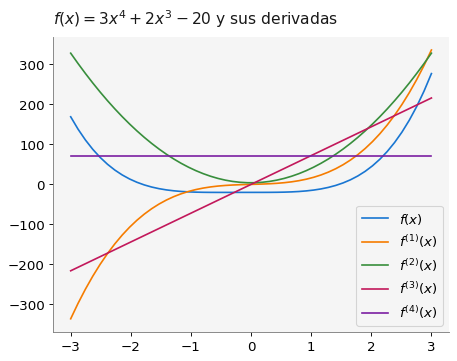
\includegraphics{01_ejercicios_derivadas_files/figure-pdf/cell-42-output-1.png}

Encuentra la primera y segunda derivada de la siguientes funciones: - a)
\(f(x)= x^5 - 2x^3 + x\) - b) \(f(x)= 4 \cos x^2\)

\begin{enumerate}
\def\labelenumi{\arabic{enumi}.}
\setcounter{enumi}{7}
\tightlist
\item
  \begin{enumerate}
  \def\labelenumii{\alph{enumii}.}
  \setcounter{enumii}{4}
  \tightlist
  \item
    \(f(x) = x^5 - 2x^3 + x, f'(x) = ¿?\)
  \end{enumerate}
\end{enumerate}

\begin{Shaded}
\begin{Highlighting}[]
\CommentTok{\# Escribe tu respuesta como sigue }
\CommentTok{\# respuesta = ...}

\CommentTok{\#\#\# }\RegionMarkerTok{BEGIN}\CommentTok{ SOLUTION}
\NormalTok{respuesta }\OperatorTok{=} \DecValTok{5}\OperatorTok{*}\NormalTok{x}\OperatorTok{**}\DecValTok{4}\OperatorTok{{-}}\DecValTok{6}\OperatorTok{*}\NormalTok{x}\OperatorTok{**}\DecValTok{2}\OperatorTok{+}\DecValTok{1}

\NormalTok{file\_answer.write(}\StringTok{\textquotesingle{}8e\textquotesingle{}}\NormalTok{, }\BuiltInTok{str}\NormalTok{(respuesta))}
\CommentTok{\#\#\# }\RegionMarkerTok{END}\CommentTok{ SOLUTION}

\NormalTok{display(respuesta)}
\end{Highlighting}
\end{Shaded}

\begin{verbatim}
El directorio :/home/jovyan/macti_notes/notebooks/.ans/Derivada/ ya existe
Respuestas y retroalimentación almacenadas.
\end{verbatim}

$\displaystyle 5 x^{4} - 6 x^{2} + 1$

\begin{Shaded}
\begin{Highlighting}[]
\NormalTok{quizz.eval\_expression(}\StringTok{\textquotesingle{}8e\textquotesingle{}}\NormalTok{, respuesta)}
\end{Highlighting}
\end{Shaded}

\begin{verbatim}
----------------------------------------
8e | Tu respuesta:
es correcta.
----------------------------------------
\end{verbatim}

$\displaystyle 5 x^{4} - 6 x^{2} + 1$

\begin{enumerate}
\def\labelenumi{\arabic{enumi}.}
\setcounter{enumi}{7}
\tightlist
\item
  \begin{enumerate}
  \def\labelenumii{\alph{enumii}.}
  \setcounter{enumii}{5}
  \tightlist
  \item
    \(f(x) = x^5 - 2x^3 + x, f''(x) = ¿?\)
  \end{enumerate}
\end{enumerate}

\begin{Shaded}
\begin{Highlighting}[]
\CommentTok{\# Escribe tu respuesta como sigue }
\CommentTok{\# respuesta = ...}

\CommentTok{\#\#\# }\RegionMarkerTok{BEGIN}\CommentTok{ SOLUTION}
\NormalTok{respuesta }\OperatorTok{=} \DecValTok{20}\OperatorTok{*}\NormalTok{x}\OperatorTok{**}\DecValTok{3}\OperatorTok{{-}}\DecValTok{12}\OperatorTok{*}\NormalTok{x}

\NormalTok{file\_answer.write(}\StringTok{\textquotesingle{}8f\textquotesingle{}}\NormalTok{, }\BuiltInTok{str}\NormalTok{(respuesta))}
\CommentTok{\#\#\# }\RegionMarkerTok{END}\CommentTok{ SOLUTION}

\NormalTok{display(respuesta)}
\end{Highlighting}
\end{Shaded}

\begin{verbatim}
El directorio :/home/jovyan/macti_notes/notebooks/.ans/Derivada/ ya existe
Respuestas y retroalimentación almacenadas.
\end{verbatim}

$\displaystyle 20 x^{3} - 12 x$

\begin{Shaded}
\begin{Highlighting}[]
\NormalTok{quizz.eval\_expression(}\StringTok{\textquotesingle{}8f\textquotesingle{}}\NormalTok{, respuesta)}
\end{Highlighting}
\end{Shaded}

\begin{verbatim}
----------------------------------------
8f | Tu respuesta:
es correcta.
----------------------------------------
\end{verbatim}

$\displaystyle 20 x^{3} - 12 x$

\begin{enumerate}
\def\labelenumi{\arabic{enumi}.}
\setcounter{enumi}{7}
\tightlist
\item
  \begin{enumerate}
  \def\labelenumii{\alph{enumii}.}
  \setcounter{enumii}{6}
  \tightlist
  \item
    \(f(x) = 4 \cos x^2, f'(x) = ¿?\)
  \end{enumerate}
\end{enumerate}

\begin{Shaded}
\begin{Highlighting}[]
\CommentTok{\# Escribe tu respuesta como sigue }
\CommentTok{\# respuesta = ...}

\CommentTok{\#\#\# }\RegionMarkerTok{BEGIN}\CommentTok{ SOLUTION}
\NormalTok{respuesta }\OperatorTok{=} \OperatorTok{{-}}\DecValTok{8} \OperatorTok{*}\NormalTok{ x }\OperatorTok{*}\NormalTok{ sy.sin(x}\OperatorTok{**}\DecValTok{2}\NormalTok{)}

\NormalTok{file\_answer.write(}\StringTok{\textquotesingle{}8g\textquotesingle{}}\NormalTok{, }\BuiltInTok{str}\NormalTok{(respuesta))}
\CommentTok{\#\#\# }\RegionMarkerTok{END}\CommentTok{ SOLUTION}

\NormalTok{display(respuesta)}
\end{Highlighting}
\end{Shaded}

\begin{verbatim}
El directorio :/home/jovyan/macti_notes/notebooks/.ans/Derivada/ ya existe
Respuestas y retroalimentación almacenadas.
\end{verbatim}

$\displaystyle - 8 x \sin{\left(x^{2} \right)}$

\begin{Shaded}
\begin{Highlighting}[]
\NormalTok{quizz.eval\_expression(}\StringTok{\textquotesingle{}8g\textquotesingle{}}\NormalTok{, respuesta)}
\end{Highlighting}
\end{Shaded}

\begin{verbatim}
----------------------------------------
8g | Tu respuesta:
es correcta.
----------------------------------------
\end{verbatim}

$\displaystyle - 8 x \sin{\left(x^{2} \right)}$

\begin{enumerate}
\def\labelenumi{\arabic{enumi}.}
\setcounter{enumi}{7}
\tightlist
\item
  \begin{enumerate}
  \def\labelenumii{\alph{enumii}.}
  \setcounter{enumii}{7}
  \tightlist
  \item
    \(f(x) = 4 \cos x^2, f''(x) = ¿?\)
  \end{enumerate}
\end{enumerate}

\begin{Shaded}
\begin{Highlighting}[]
\CommentTok{\# Escribe tu respuesta como sigue }
\CommentTok{\# respuesta = ...}

\CommentTok{\#\#\# }\RegionMarkerTok{BEGIN}\CommentTok{ SOLUTION}
\NormalTok{respuesta }\OperatorTok{=} \OperatorTok{{-}}\DecValTok{8}\OperatorTok{*}\NormalTok{sy.sin(x}\OperatorTok{**}\DecValTok{2}\NormalTok{) }\OperatorTok{{-}} \DecValTok{16}\OperatorTok{*}\NormalTok{x}\OperatorTok{**}\DecValTok{2}\OperatorTok{*}\NormalTok{sy.cos(x}\OperatorTok{**}\DecValTok{2}\NormalTok{)}

\NormalTok{file\_answer.write(}\StringTok{\textquotesingle{}8h\textquotesingle{}}\NormalTok{, }\BuiltInTok{str}\NormalTok{(respuesta))}
\CommentTok{\#\#\# }\RegionMarkerTok{END}\CommentTok{ SOLUTION}

\NormalTok{display(respuesta)}
\end{Highlighting}
\end{Shaded}

\begin{verbatim}
El directorio :/home/jovyan/macti_notes/notebooks/.ans/Derivada/ ya existe
Respuestas y retroalimentación almacenadas.
\end{verbatim}

$\displaystyle - 16 x^{2} \cos{\left(x^{2} \right)} - 8 \sin{\left(x^{2} \right)}$

\begin{Shaded}
\begin{Highlighting}[]
\NormalTok{quizz.eval\_expression(}\StringTok{\textquotesingle{}8h\textquotesingle{}}\NormalTok{, respuesta)}
\end{Highlighting}
\end{Shaded}

\begin{verbatim}
----------------------------------------
8h | Tu respuesta:
es correcta.
----------------------------------------
\end{verbatim}

$\displaystyle - 16 x^{2} \cos{\left(x^{2} \right)} - 8 \sin{\left(x^{2} \right)}$

Realiza las gráficas de las dos funciones y de su primera y segunda
derivadas.

\begin{Shaded}
\begin{Highlighting}[]
\NormalTok{f }\OperatorTok{=} \KeywordTok{lambda}\NormalTok{ x: x}\OperatorTok{**}\DecValTok{5} \OperatorTok{{-}} \DecValTok{2}\OperatorTok{*}\NormalTok{x}\OperatorTok{**}\DecValTok{3} \OperatorTok{+}\NormalTok{ x}

\CommentTok{\#\#\# }\RegionMarkerTok{BEGIN}\CommentTok{ SOLUTION}
\NormalTok{f1 }\OperatorTok{=} \KeywordTok{lambda}\NormalTok{ x: }\DecValTok{5}\OperatorTok{*}\NormalTok{x}\OperatorTok{**}\DecValTok{4} \OperatorTok{{-}}\DecValTok{6}\OperatorTok{*}\NormalTok{x}\OperatorTok{**}\DecValTok{2} \OperatorTok{+} \DecValTok{1}
\NormalTok{f2 }\OperatorTok{=} \KeywordTok{lambda}\NormalTok{ x: }\DecValTok{20}\OperatorTok{*}\NormalTok{x}\OperatorTok{**}\DecValTok{3} \OperatorTok{{-}} \DecValTok{12}\OperatorTok{*}\NormalTok{x}
\CommentTok{\#\#\# }\RegionMarkerTok{END}\CommentTok{ SOLUTION}
\CommentTok{\# f1 = lambda x: ...}
\CommentTok{\# f2 = lambda x: ...}

\CommentTok{\# Definimos la segunda función y sus derivadas}
\NormalTok{g }\OperatorTok{=} \KeywordTok{lambda}\NormalTok{ x: }\DecValTok{4}\OperatorTok{*}\NormalTok{np.cos(x}\OperatorTok{**}\DecValTok{2}\NormalTok{)}

\CommentTok{\#\#\# }\RegionMarkerTok{BEGIN}\CommentTok{ SOLUTION}
\NormalTok{g1 }\OperatorTok{=} \KeywordTok{lambda}\NormalTok{ x: }\OperatorTok{{-}}\DecValTok{8}\OperatorTok{*}\NormalTok{x}\OperatorTok{*}\NormalTok{np.sin(x}\OperatorTok{**}\DecValTok{2}\NormalTok{)}
\NormalTok{g2 }\OperatorTok{=} \KeywordTok{lambda}\NormalTok{ x: }\OperatorTok{{-}}\DecValTok{8}\OperatorTok{*}\NormalTok{np.sin(x}\OperatorTok{**}\DecValTok{2}\NormalTok{) }\OperatorTok{{-}} \DecValTok{16}\OperatorTok{*}\NormalTok{x}\OperatorTok{**}\DecValTok{2}\OperatorTok{*}\NormalTok{np.cos(x}\OperatorTok{**}\DecValTok{2}\NormalTok{)}
\CommentTok{\#\#\# }\RegionMarkerTok{END}\CommentTok{ SOLUTION}
\CommentTok{\# g1 = lambda x: ...}
\CommentTok{\# g2 = lambda x: ...}

\NormalTok{xc }\OperatorTok{=}\NormalTok{ np.linspace(}\OperatorTok{{-}}\DecValTok{3}\NormalTok{, }\DecValTok{3}\NormalTok{, }\DecValTok{50}\NormalTok{) }\CommentTok{\# Codominio de las funciones}

\CommentTok{\# Graficamos las funciones y sus derivadas}
\NormalTok{plt.figure(figsize}\OperatorTok{=}\NormalTok{(}\DecValTok{16}\NormalTok{,}\DecValTok{6}\NormalTok{))}
\NormalTok{ax1 }\OperatorTok{=}\NormalTok{ plt.subplot(}\DecValTok{1}\NormalTok{,}\DecValTok{2}\NormalTok{,}\DecValTok{1}\NormalTok{)}
\NormalTok{ax2 }\OperatorTok{=}\NormalTok{ plt.subplot(}\DecValTok{1}\NormalTok{,}\DecValTok{2}\NormalTok{,}\DecValTok{2}\NormalTok{)}

\NormalTok{ax1.plot(xc, f(xc), label}\OperatorTok{=}\StringTok{\textquotesingle{}$f(x)$\textquotesingle{}}\NormalTok{,lw}\OperatorTok{=}\DecValTok{3}\NormalTok{)}
\NormalTok{ax1.plot(xc, f1(xc), label}\OperatorTok{=}\StringTok{\textquotesingle{}$f\^{}\{(1)\}(x)$\textquotesingle{}}\NormalTok{,lw}\OperatorTok{=}\DecValTok{3}\NormalTok{)}
\NormalTok{ax1.plot(xc, f2(xc), label}\OperatorTok{=}\StringTok{\textquotesingle{}$f\^{}\{(2)\}(x)$\textquotesingle{}}\NormalTok{,lw}\OperatorTok{=}\DecValTok{3}\NormalTok{)}
\NormalTok{ax1.legend(loc}\OperatorTok{=}\StringTok{\textquotesingle{}upper center\textquotesingle{}}\NormalTok{)}
\NormalTok{ax1.set\_title(}\StringTok{\textquotesingle{}$f(x)=x\^{}5 {-} 2x\^{}3 + x$ y sus derivadas\textquotesingle{}}\NormalTok{)}
\NormalTok{ax1.set\_xlabel}

\NormalTok{ax2.plot(xc, g(xc), label}\OperatorTok{=}\StringTok{\textquotesingle{}$g(x)$\textquotesingle{}}\NormalTok{,lw}\OperatorTok{=}\DecValTok{3}\NormalTok{)}
\NormalTok{ax2.plot(xc, g1(xc), label}\OperatorTok{=}\StringTok{\textquotesingle{}$g\^{}\{(1)\}(x)$\textquotesingle{}}\NormalTok{,lw}\OperatorTok{=}\DecValTok{3}\NormalTok{)}
\NormalTok{ax2.plot(xc, g2(xc), label}\OperatorTok{=}\StringTok{\textquotesingle{}$g\^{}\{(2)\}(x)$\textquotesingle{}}\NormalTok{,lw}\OperatorTok{=}\DecValTok{3}\NormalTok{)}
\NormalTok{ax2.legend(loc}\OperatorTok{=}\StringTok{\textquotesingle{}upper center\textquotesingle{}}\NormalTok{)}
\NormalTok{ax2.set\_title(}\StringTok{\textquotesingle{}$g(x)=4\textbackslash{}cos(x\^{}2)$ y sus derivadas\textquotesingle{}}\NormalTok{)}

\NormalTok{ax1.set\_xlabel(}\StringTok{"$x$"}\NormalTok{)}
\NormalTok{ax1.set\_ylabel(}\StringTok{"$f(x)$"}\NormalTok{)}
\NormalTok{ax2.set\_xlabel(}\StringTok{"$x$"}\NormalTok{)}
\NormalTok{ax2.set\_ylabel(}\StringTok{"$g(x)$"}\NormalTok{)}

\NormalTok{plt.show()}
\end{Highlighting}
\end{Shaded}

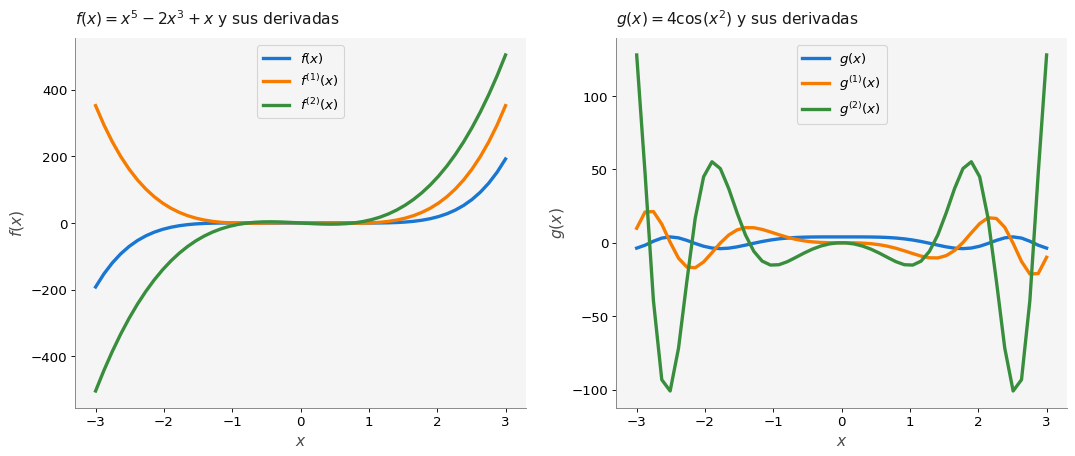
\includegraphics{01_ejercicios_derivadas_files/figure-pdf/cell-51-output-1.png}

\#\#\# 9. Aplicación de la regla de L'Hopital

Utilizando la regla de L'Hopital encuentra el límite de
\(\displaystyle f(x)=\frac{\sin(x)}{x}\) cuando \(x\) tiende a cero.

\textbf{Solución.}

Al cumplirse las condiciones de la regla podemos asegurar que:
\[ \lim_{x \to 0} \frac{\sin (x)}{x} = \lim_{x \to 0} \frac{\sin^\prime(x)}{x^\prime} = \lim_{x \to 0} \frac{\cos(x)}{1}=1\]

\begin{Shaded}
\begin{Highlighting}[]
\NormalTok{f }\OperatorTok{=} \KeywordTok{lambda}\NormalTok{ x: np.sin(x) }\OperatorTok{/}\NormalTok{ x}

\NormalTok{x }\OperatorTok{=}\NormalTok{ np.linspace(}\OperatorTok{{-}}\DecValTok{4}\OperatorTok{*}\NormalTok{np.pi, }\DecValTok{4}\OperatorTok{*}\NormalTok{np.pi, num}\OperatorTok{=}\DecValTok{100}\NormalTok{) }\CommentTok{\# Codominio de la función}

\CommentTok{\# Graficamos la función y el punto (0, f(0))}
\NormalTok{plt.title(}\StringTok{\textquotesingle{}$f(x)=\textbackslash{}sin(x) / x$\textquotesingle{}}\NormalTok{)}
\NormalTok{plt.ylabel(}\StringTok{"$f(x)$"}\NormalTok{)}
\NormalTok{plt.xlabel(}\StringTok{"$x$"}\NormalTok{)}
\NormalTok{plt.plot(x, f(x),lw}\OperatorTok{=}\DecValTok{3}\NormalTok{)}
\NormalTok{plt.scatter(}\DecValTok{0}\NormalTok{, }\DecValTok{1}\NormalTok{, label}\OperatorTok{=}\StringTok{\textquotesingle{}Límite cuando $x \textbackslash{}Rightarrow 0$\textquotesingle{}}\NormalTok{, fc}\OperatorTok{=}\StringTok{\textquotesingle{}red\textquotesingle{}}\NormalTok{, ec}\OperatorTok{=}\StringTok{\textquotesingle{}black\textquotesingle{}}\NormalTok{, alpha}\OperatorTok{=}\FloatTok{0.75}\NormalTok{, s}\OperatorTok{=}\DecValTok{75}\NormalTok{, zorder}\OperatorTok{=}\DecValTok{10}\NormalTok{)}
\NormalTok{plt.legend()}
\NormalTok{plt.show()}
\end{Highlighting}
\end{Shaded}

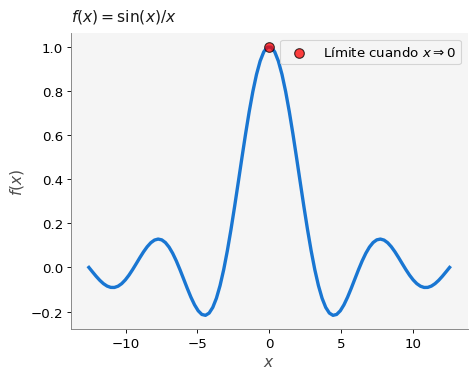
\includegraphics{01_ejercicios_derivadas_files/figure-pdf/cell-52-output-1.png}

\#\#\# 10. Ejemplo del teorema de Rolle. Considere la función
\(f(x)= x^2 + 5\), la cual es continúa en todo \(\mathbb{R}\). Tomemos
el intervalo \([-5,5]\) y hagamos la gráfica de esta función. Observe en
la gráfica que sigue, que se cumplen las condiciones del Teorema de
Rolle y por lo tanto es posible encontrar un punto \(c\), punto rojo,
donde la derivada es cero (línea roja).

\begin{Shaded}
\begin{Highlighting}[]
\CommentTok{\# Dominio e imagen de la gráfica}
\NormalTok{xc }\OperatorTok{=}\NormalTok{ np.linspace(}\OperatorTok{{-}}\DecValTok{10}\NormalTok{,}\DecValTok{10}\NormalTok{,}\DecValTok{200}\NormalTok{)}
\NormalTok{f }\OperatorTok{=} \KeywordTok{lambda}\NormalTok{ i: i}\OperatorTok{**}\DecValTok{2} \OperatorTok{+} \DecValTok{5} 

\CommentTok{\# Configuración de la grafica}
\NormalTok{plt.xticks(}\BuiltInTok{range}\NormalTok{(}\OperatorTok{{-}}\DecValTok{10}\NormalTok{,}\DecValTok{11}\NormalTok{,}\DecValTok{5}\NormalTok{))}
\NormalTok{plt.yticks(}\BuiltInTok{range}\NormalTok{(}\OperatorTok{{-}}\DecValTok{10}\NormalTok{,}\DecValTok{110}\NormalTok{,}\DecValTok{10}\NormalTok{))}
\NormalTok{plt.xlabel(}\StringTok{"$x$"}\NormalTok{,)}
\NormalTok{plt.ylabel(}\StringTok{"$f(x)$"}\NormalTok{)}
\NormalTok{plt.title(}\StringTok{"$f(x)=x\^{}}\SpecialCharTok{\{2\}}\StringTok{+5$"}\NormalTok{)}

\CommentTok{\# Función}
\NormalTok{plt.plot(xc,f(xc))}

\CommentTok{\# Dibujamos algunas líneas en la gráfica}
\NormalTok{plt.plot(np.linspace(}\OperatorTok{{-}}\DecValTok{10}\NormalTok{,}\DecValTok{10}\NormalTok{,}\DecValTok{2}\NormalTok{),[f(}\DecValTok{5}\NormalTok{)]}\OperatorTok{*}\DecValTok{2}\NormalTok{,ls}\OperatorTok{=}\StringTok{"dashed"}\NormalTok{,color}\OperatorTok{=}\StringTok{"green"}\NormalTok{)}
\NormalTok{plt.plot((}\DecValTok{5}\NormalTok{,}\DecValTok{5}\NormalTok{),(}\DecValTok{0}\NormalTok{,f(}\DecValTok{5}\NormalTok{)),ls}\OperatorTok{=}\StringTok{"dashed"}\NormalTok{,color}\OperatorTok{=}\StringTok{"green"}\NormalTok{)}
\NormalTok{plt.plot((}\OperatorTok{{-}}\DecValTok{5}\NormalTok{,}\OperatorTok{{-}}\DecValTok{5}\NormalTok{),(}\DecValTok{0}\NormalTok{,f(}\DecValTok{5}\NormalTok{)),ls}\OperatorTok{=}\StringTok{"dashed"}\NormalTok{,color}\OperatorTok{=}\StringTok{"green"}\NormalTok{)}
\NormalTok{plt.plot((}\OperatorTok{{-}}\DecValTok{3}\NormalTok{,}\DecValTok{3}\NormalTok{),(}\DecValTok{5}\NormalTok{,}\DecValTok{5}\NormalTok{),color}\OperatorTok{=}\StringTok{"red"}\NormalTok{,label}\OperatorTok{=}\StringTok{"Línea Tangente"}\NormalTok{)}

\CommentTok{\# Dibujamos algunos puntos en la gráfica}
\NormalTok{plt.scatter((}\OperatorTok{{-}}\DecValTok{5}\NormalTok{,}\DecValTok{5}\NormalTok{),(}\DecValTok{0}\NormalTok{,}\DecValTok{0}\NormalTok{),color}\OperatorTok{=}\StringTok{"black"}\NormalTok{,label}\OperatorTok{=}\StringTok{"Puntos a y b"}\NormalTok{,zorder}\OperatorTok{=}\DecValTok{5}\NormalTok{)}
\NormalTok{plt.scatter((}\OperatorTok{{-}}\DecValTok{5}\NormalTok{,}\DecValTok{5}\NormalTok{),(f(}\OperatorTok{{-}}\DecValTok{5}\NormalTok{),f(}\DecValTok{5}\NormalTok{)),color}\OperatorTok{=}\StringTok{"blue"}\NormalTok{,label}\OperatorTok{=}\StringTok{"Puntos $f(a)$ y $f(b)$"}\NormalTok{,zorder}\OperatorTok{=}\DecValTok{5}\NormalTok{)}
\NormalTok{plt.scatter(}\DecValTok{0}\NormalTok{,f(}\DecValTok{0}\NormalTok{),color}\OperatorTok{=}\StringTok{"red"}\NormalTok{,label}\OperatorTok{=}\StringTok{"Punto en el que $f\textquotesingle{}(x)=0$"}\NormalTok{,zorder}\OperatorTok{=}\DecValTok{5}\NormalTok{)}

\NormalTok{plt.legend(loc}\OperatorTok{=}\StringTok{"upper center"}\NormalTok{)}
\NormalTok{plt.show()}
\end{Highlighting}
\end{Shaded}

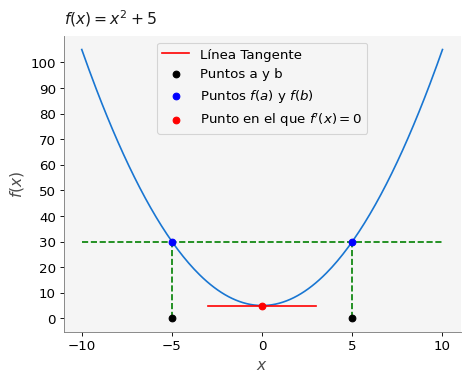
\includegraphics{01_ejercicios_derivadas_files/figure-pdf/cell-53-output-1.png}

\# Reglas de derivación

En general no es complicado calcular la derivada de cualquier función y
existen reglas para hacerlo más fácil.

\textbf{Regla de potencias}

Para cualquier número real \(n\) si \(f(x)= x^n\), entonces \[
f^\prime(x) = n x^{n-1}
\]

\textbf{Regla de la función constante}

Si \(f(x)=c\) es una función constante, entonces \[ 
f^\prime(x)=0 
\]

\textbf{Regla de la multiplicación por constante}

Si \(c\) es cualquier constante y \(f(x)\) es diferenciable, entonces
\(g(x)= c f(x)\) también es diferenciable y su derivada es: \[ 
g^\prime(x) = c f^\prime(x) 
\]

\textbf{Regla de suma y diferencia}

Si \(f(x)\) y \(g(x)\) son diferenciables, entonces \(f(x) + g(x)\) y
\(f(x) - g(x)\) también son diferenciables y sus derivadas son: \[ 
[f(x)+ g(x)]^\prime = f^\prime(x) + g^\prime(x) 
\]

\[ 
[f(x)- g(x)]^\prime=f^\prime(x) - g^\prime(x) 
\]

\textbf{Regla del producto}

Si \(f(x)\) y \(g(x)\) son funciones diferenciables, entonces
\(f(x)g(x)\) es diferenciable y su derivada es: \[ 
[f(x) g(x)]^\prime= f(x)g^\prime(x) + g(x)f^\prime(x) 
\]

\textbf{Regla del cociente}

Si \(f\) y \(g\) son funciones diferenciables y \(g(x) \neq 0\),
entonces \(f(x)/g(x)\) es diferenciable y su derivada es: \[  
\left[\frac{f(x)}{g(x)} \right]^\prime = \frac{f(x)g^\prime(x)- f^\prime(x)g(x) }{g(x)^2}
\]

\textbf{Regla de la cadena}

Si la función \(f(u)\) es diferenciable, donde \(u = g(x)\), y la
función \(g(x)\) es diferenciable, entonces la composición
\(y=(f \circ g)(x)= f(g(x))\) es diferenciable: \[ 
f(g(x))^\prime = f^\prime(g(x)) \cdot g^\prime(x)  
\]

\textbf{Regla de L'Hôpital}

Esta regla es utilizada en caso de indeterminaciones donde \(f(x)\) y
\(g(x)\) son dos funciones continuas definidas en el intervalo
\([a,b]\), derivables en \((a,b)\) y sea \(c\) perteneciente a \((a,b)\)
tal que \(f(c)=g(c)=0\) y \(g^\prime(x) \neq 0\) si \(x \neq c\). Si
existe el límite \(L\) de \(f^\prime/g^\prime\) en \(c\), entonces
existe el límite de \(f(x)/g(x)\) (en \(c\)) y es igual a \(L\). Por lo
tanto: \[ 
\lim_{x \to c} \frac{f(x)}{g(x)} = \lim_{x \to c} \frac{f^\prime(x)}{g^\prime(x)} = L 
\]

\textbf{Derivadas de funciones trigonométricas}

\[
\begin{eqnarray}
\sin^\prime(x) & = & \cos(x) \\ 
\cos^\prime(x) & = & -\sin(x) \\
\tan^\prime(x) & = & \sec^2(x) \\
\sec^\prime(x) & = & \sec(x)\tan(x) \\
\cot^\prime(x) & = & -\csc^2(x) \\
\csc^\prime(x) & = & -\csc(x)\cot(x)
\end{eqnarray}
\]

\textbf{Derivada la función exponencial}

\[
\left[ e^{x} \right]^\prime = e^{x}
\]

\# Teorema de Rolle : Sea \(a < b\) y suponga que
\(f : [a, b] → {\mathbb{R}}\) es derivable en \((a, b)\) y continua en
\([a, b]\) y \(f(a) = f(b)\). Entonces \(∃ x_0 ∈ (a, b)\) tal que
\(f^\prime(x_0) = 0\)

Lo anterior quiere decir que, dadas las condiciones del teorema, es
posible encontrar un punto de la función \(f(x)\) dentro del intervalo
\((a,b)\) donde la derivada es cero; en otras palabras, en ese punto de
la función la línea tangente es horizontal

\# Derivadas de orden superior

Es posible obtener la derivada de la derivada, es decir, si tenemos una
función \(f(x)\) cuya derivada es \(f^\prime(x)\), entonces podemos
calcular la derivada a esta última función, para obtener
\(f^{\prime\prime}(x)\), a esta última función, si es que existe, se le
conoce como la segunda derivada de \(f(x)\). También se puede denotar a
la segunda derivada com \(f^{(2)}(x)\).

En general, si \(f(x)\) es derivable \(k\) veces, entonces es posible
obtener la \(k\)-ésima derivada de dicha función, que se escribe como:
\[ 
\frac{d^kf(x)}{dx^k} = f^{(k)}(x)
\]

\bookmarksetup{startatroot}

\chapter{La derivada de una función y su
aproximación}\label{la-derivada-de-una-funciuxf3n-y-su-aproximaciuxf3n}

\textbf{Objetivo}. - Revisar el concepto de derivada usando herramientas
visuales que permitan comprender su sentido geométrico y comprender lo
que significa el cambio instantáneo.

MACTI-Analisis\_Numerico\_01 by Luis M. de la Cruz is licensed under
Attribution-ShareAlike 4.0 International

Trabajo realizado con el apoyo del Programa UNAM-DGAPA-PAPIME PE101922

\begin{Shaded}
\begin{Highlighting}[]
\CommentTok{\# Importamos todas las bibliotecas}
\ImportTok{import}\NormalTok{ matplotlib.pyplot }\ImportTok{as}\NormalTok{ plt}
\ImportTok{import}\NormalTok{ numpy }\ImportTok{as}\NormalTok{ np}
\ImportTok{import}\NormalTok{ pandas }\ImportTok{as}\NormalTok{ pd}
\ImportTok{import}\NormalTok{ sympy }\ImportTok{as}\NormalTok{ sy}
\ImportTok{import}\NormalTok{ macti.visual}
\ImportTok{from}\NormalTok{ macti.evaluation }\ImportTok{import} \OperatorTok{*}
\end{Highlighting}
\end{Shaded}

\begin{Shaded}
\begin{Highlighting}[]
\NormalTok{quizz }\OperatorTok{=}\NormalTok{ Quizz(}\StringTok{\textquotesingle{}q2\textquotesingle{}}\NormalTok{, }\StringTok{\textquotesingle{}notebooks\textquotesingle{}}\NormalTok{, }\StringTok{\textquotesingle{}local\textquotesingle{}}\NormalTok{)}
\end{Highlighting}
\end{Shaded}

\#\# Introducción

Si revisamos con cuidado, algunas definiciones matemáticas utilizan un
tipo de figura literaria conocida como \emph{oxímoron}. En términos
simples, un oxímoron consiste en usar dos conceptos de significado
opuesto y con ello generar un tercer concepto.

Por ejemplo: \textbf{La razón de cambio instantáneo}. - Cuando se habla
de un \emph{cambio}, se requiere de la comparación entre dos o más
estados y con ello analizar las diferencias entre un estado y otro; -
por otro lado, la palabra \emph{instantáneo} tiene que ver con algo que
dura un solo instante, es decir un tiempo puntal.

Entonces el concepto ``\textbf{cambio instantáneo}'' representa un
oxímoron. Pero ¿cuál es su significado? ¿Será importante este concepto
en nuestra vida diaria?

En lo que sigue veremos que la razón de cambio instantáneo tiene que ver
con un concepto muy importante en Cálculo: \textbf{la derivada}.

\#\# La curva del olvido.

Un estudiante de lenguas participará en un concurso internacional cuyo
principal reto es el conocimiento del vocabulario de un cierto idioma.
Por ello, es importante que el estudiante utilice un método de estudio
adecuado para recordar el significado del mayor número de palabras
posible.

La curva del olvido puede ayudar al estudiante a generar un plan de
estudio adecuado. La función que define esta curva es la siguiente:

\[
R(t) = e^{-t/S}
\]

donde \(R\) es cuanto recordamos, \(S\) es la intensidad del recuerdo y
\(t\) el tiempo. Podemos definir \(S \in (0,1]\), donde \(1\) es la
máxima intensidad de recuerdo y un valor cercano a \(0\) corresponde a
algo que no nos interesa nada.

\textbf{Observación}: \(S\) no puede ser exactamente \(0\) por que en
ese caso la función \(R(t)\) no está definida.

La siguiente gráfica muestra cómo decrecen nuestros recuerdos con el
paso del tiempo.

\begin{Shaded}
\begin{Highlighting}[]
\CommentTok{\# Primero definimos la función del olvido}
\KeywordTok{def}\NormalTok{ R(t, S}\OperatorTok{=}\FloatTok{0.9}\NormalTok{):}
    \ControlFlowTok{return}\NormalTok{ np.exp(}\OperatorTok{{-}}\NormalTok{t}\OperatorTok{/}\NormalTok{S)}

\CommentTok{\# Dominio de tiempo (hasta 7 días).}
\NormalTok{t }\OperatorTok{=}\NormalTok{ np.linspace(}\DecValTok{0}\NormalTok{,}\DecValTok{7}\NormalTok{,}\DecValTok{100}\NormalTok{)}

\CommentTok{\# Tres curvas del olvido para tres valores de S}
\NormalTok{plt.plot(t, R(t,}\FloatTok{0.1}\NormalTok{), lw}\OperatorTok{=}\DecValTok{3}\NormalTok{, c}\OperatorTok{=}\StringTok{\textquotesingle{}C3\textquotesingle{}}\NormalTok{, label}\OperatorTok{=}\StringTok{\textquotesingle{}}\SpecialCharTok{\{\}}\StringTok{\textquotesingle{}}\NormalTok{.}\BuiltInTok{format}\NormalTok{(}\FloatTok{0.1}\NormalTok{))}
\NormalTok{plt.plot(t, R(t,}\FloatTok{0.5}\NormalTok{), lw}\OperatorTok{=}\DecValTok{3}\NormalTok{, c}\OperatorTok{=}\StringTok{\textquotesingle{}C2\textquotesingle{}}\NormalTok{, label}\OperatorTok{=}\StringTok{\textquotesingle{}}\SpecialCharTok{\{\}}\StringTok{\textquotesingle{}}\NormalTok{.}\BuiltInTok{format}\NormalTok{(}\FloatTok{0.5}\NormalTok{))}
\NormalTok{plt.plot(t, R(t,}\FloatTok{0.9}\NormalTok{), lw}\OperatorTok{=}\DecValTok{3}\NormalTok{, c}\OperatorTok{=}\StringTok{\textquotesingle{}C1\textquotesingle{}}\NormalTok{, label}\OperatorTok{=}\StringTok{\textquotesingle{}}\SpecialCharTok{\{\}}\StringTok{\textquotesingle{}}\NormalTok{.}\BuiltInTok{format}\NormalTok{(}\FloatTok{0.9}\NormalTok{))}

\CommentTok{\# Configuración de la gráfica. }
\NormalTok{plt.title(}\StringTok{"Función del olvido: $R(t)=e\^{}\{{-}t/S\}$"}\NormalTok{)}
\NormalTok{plt.ylabel(}\StringTok{"$R(t)$"}\NormalTok{)}
\NormalTok{plt.xlabel(}\StringTok{"$t$ [días]"}\NormalTok{)}
\NormalTok{plt.legend(title }\OperatorTok{=} \StringTok{\textquotesingle{}Intensidad $S$\textquotesingle{}}\NormalTok{)}
\NormalTok{plt.grid()}
\NormalTok{plt.show()}
\end{Highlighting}
\end{Shaded}

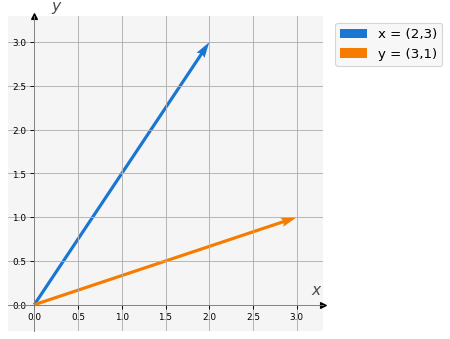
\includegraphics{02_aproximacion_de_derivada_files/figure-pdf/cell-4-output-1.png}

\#\#\# ¿Cuánto tiempo dura el recuerdo?

¿Será posible determinar cada cuanto tiempo el estudiante debe repasar
las palabras para que no las olvide y pueda ganar el concurso? ¿De qué
depende esto?

Tomemos por ejemplo el caso de \(S=0.9\) (curva naranja). ¿En qué parte
de la gráfica se incrementa el olvido? en otras palabras ¿en qué parte
de la gráfica el descenso es más rápido?

Para conocer ese descenso, debemos calcular la pendiente \(m\) y eso lo
podemos hacer con la siguiente fórmula:

\[
m = \frac{R(t_2) - R(t_1)}{t_2 - t_1} \tag{1}
\]

donde \(t_1\) y \(t_2\) son dos tiempos distintos.

Si definimos \(h = t_2 - t_1\) y \(t = t_1\) podemos escribir la fórmula
\((1)\) como sigue:

\[
m(t) = \frac{R(t + h) - R(t)}{h} \tag{2}
\]

En esta última fórmula vemos que la pendiente depende de \(t\), es
decir, en qué día nos encontramos.

Vamos a calcular \(R(t)\) y \(m(t)\) en \(t = [0,1,2,3,4,5,6,7]\), para
\(h = 1\) :

\begin{Shaded}
\begin{Highlighting}[]
\NormalTok{h }\OperatorTok{=} \FloatTok{1.0}
\NormalTok{td }\OperatorTok{=}\NormalTok{ np.arange(}\DecValTok{0}\NormalTok{,}\DecValTok{8}\NormalTok{,h) }\CommentTok{\# Definición de las t = 0,1,2,...,7}
\NormalTok{r }\OperatorTok{=}\NormalTok{ np.zeros(}\BuiltInTok{len}\NormalTok{(td)) }\CommentTok{\# Arreglo para almacenar el valor de R}
\NormalTok{m }\OperatorTok{=}\NormalTok{ np.zeros(}\BuiltInTok{len}\NormalTok{(td)) }\CommentTok{\# Arreglo para almacenar las pendientes}

\BuiltInTok{print}\NormalTok{(}\StringTok{\textquotesingle{}td = }\SpecialCharTok{\{\}}\StringTok{\textquotesingle{}}\NormalTok{.}\BuiltInTok{format}\NormalTok{(td))}
\BuiltInTok{print}\NormalTok{(}\StringTok{\textquotesingle{}r = }\SpecialCharTok{\{\}}\StringTok{\textquotesingle{}}\NormalTok{.}\BuiltInTok{format}\NormalTok{(r))}
\BuiltInTok{print}\NormalTok{(}\StringTok{\textquotesingle{}m = }\SpecialCharTok{\{\}}\StringTok{\textquotesingle{}}\NormalTok{.}\BuiltInTok{format}\NormalTok{(m))}
\end{Highlighting}
\end{Shaded}

\begin{verbatim}
td = [0. 1. 2. 3. 4. 5. 6. 7.]
r = [0. 0. 0. 0. 0. 0. 0. 0.]
m = [0. 0. 0. 0. 0. 0. 0. 0.]
\end{verbatim}

\begin{Shaded}
\begin{Highlighting}[]
\CommentTok{\# Hacemos los cálculos en cada uno de los días}
\ControlFlowTok{for}\NormalTok{ i, t }\KeywordTok{in} \BuiltInTok{enumerate}\NormalTok{(td):}
\NormalTok{    r[i] }\OperatorTok{=}\NormalTok{ R(t)                  }\CommentTok{\# Función del olvido}
\NormalTok{    m[i] }\OperatorTok{=}\NormalTok{ (R(t }\OperatorTok{+}\NormalTok{ h) }\OperatorTok{{-}}\NormalTok{ R(t)) }\OperatorTok{/}\NormalTok{ h }\CommentTok{\# Pendiente}

\CommentTok{\# Ponemos la información en un DataFrame y la mostramos}
\NormalTok{tabla }\OperatorTok{=}\NormalTok{ pd.DataFrame(np.array([td, r, m]).T, }
\NormalTok{                     columns }\OperatorTok{=}\NormalTok{ [}\StringTok{\textquotesingle{}$t$\textquotesingle{}}\NormalTok{, }\StringTok{\textquotesingle{}$R(t)$\textquotesingle{}}\NormalTok{, }\StringTok{\textquotesingle{}$m(t)$\textquotesingle{}}\NormalTok{])}
\NormalTok{tabla}
\end{Highlighting}
\end{Shaded}

\begin{longtable}[]{@{}llll@{}}
\toprule\noalign{}
& \$t\$ & \$R(t)\$ & \$m(t)\$ \\
\midrule\noalign{}
\endhead
\bottomrule\noalign{}
\endlastfoot
0 & 0.0 & 1.000000 & -0.670807 \\
1 & 1.0 & 0.329193 & -0.220825 \\
2 & 2.0 & 0.108368 & -0.072694 \\
3 & 3.0 & 0.035674 & -0.023930 \\
4 & 4.0 & 0.011744 & -0.007878 \\
5 & 5.0 & 0.003866 & -0.002593 \\
6 & 6.0 & 0.001273 & -0.000854 \\
7 & 7.0 & 0.000419 & -0.000281 \\
\end{longtable}

Observa que la pendiente es negativa, lo cual indica un decrecimiento.
También la magnitud de la pendiente (su valor absoluto) disminuye
conforme \(t\) avanza. Vemos que el recuerdo disminuye mucho al
principio, de tal manera que en el tercer día ya casi no se recuerda
nada, alrededor del \(3.5\%\). Esto se ve de manera gráfica como sigue:

\begin{Shaded}
\begin{Highlighting}[]
\CommentTok{\# Dominio de tiempo (hasta 7 días).}
\NormalTok{t }\OperatorTok{=}\NormalTok{ np.linspace(}\DecValTok{0}\NormalTok{,}\DecValTok{7}\NormalTok{,}\DecValTok{100}\NormalTok{)}

\CommentTok{\# La curva del olvido para S = 0.9}
\NormalTok{plt.plot(t, R(t), lw}\OperatorTok{=}\DecValTok{3}\NormalTok{, c}\OperatorTok{=}\StringTok{\textquotesingle{}C1\textquotesingle{}}\NormalTok{)}

\CommentTok{\# Línea punteada}
\NormalTok{plt.plot([}\DecValTok{0}\NormalTok{,}\DecValTok{1}\NormalTok{,}\DecValTok{2}\NormalTok{,}\DecValTok{3}\NormalTok{], [R(}\DecValTok{0}\NormalTok{), R(}\DecValTok{1}\NormalTok{), R(}\DecValTok{2}\NormalTok{), R(}\DecValTok{3}\NormalTok{)], }\StringTok{\textquotesingle{}o{-}{-}\textquotesingle{}}\NormalTok{, lw}\OperatorTok{=}\DecValTok{1}\NormalTok{, zorder}\OperatorTok{=}\DecValTok{5}\NormalTok{)}

\CommentTok{\# Configuración de la gráfica. }
\NormalTok{plt.title(}\StringTok{"Función del olvido: $R(t)=e\^{}\{{-}t/S\}$, para $S = 0.9$"}\NormalTok{)}
\NormalTok{plt.ylabel(}\StringTok{"$R(t)$"}\NormalTok{)}
\NormalTok{plt.xlabel(}\StringTok{"$t$ [días]"}\NormalTok{)}

\CommentTok{\# Información de los primeros 3 días}
\NormalTok{plt.text(}\DecValTok{2}\NormalTok{,}\FloatTok{0.6}\NormalTok{,}\StringTok{\textquotesingle{}$R$(}\SpecialCharTok{\{2:\}}\StringTok{) = }\SpecialCharTok{\{0:5.4f\}}\StringTok{,}\CharTok{\textbackslash{}t}\StringTok{ $m$(}\SpecialCharTok{\{2:\}}\StringTok{) = }\SpecialCharTok{\{1:5.4f\}}\StringTok{\textquotesingle{}}\NormalTok{.}\BuiltInTok{format}\NormalTok{(R(}\DecValTok{0}\NormalTok{), m[}\DecValTok{0}\NormalTok{], }\DecValTok{0}\NormalTok{))}
\NormalTok{plt.text(}\DecValTok{2}\NormalTok{,}\FloatTok{0.5}\NormalTok{,}\StringTok{\textquotesingle{}$R$(}\SpecialCharTok{\{2:\}}\StringTok{) = }\SpecialCharTok{\{0:5.4f\}}\StringTok{,}\CharTok{\textbackslash{}t}\StringTok{ $m$(}\SpecialCharTok{\{2:\}}\StringTok{) = }\SpecialCharTok{\{1:5.4f\}}\StringTok{\textquotesingle{}}\NormalTok{.}\BuiltInTok{format}\NormalTok{(R(}\DecValTok{1}\NormalTok{), m[}\DecValTok{1}\NormalTok{], }\DecValTok{1}\NormalTok{))}
\NormalTok{plt.text(}\DecValTok{2}\NormalTok{,}\FloatTok{0.4}\NormalTok{,}\StringTok{\textquotesingle{}$R$(}\SpecialCharTok{\{2:\}}\StringTok{) = }\SpecialCharTok{\{0:5.4f\}}\StringTok{,}\CharTok{\textbackslash{}t}\StringTok{ $m$(}\SpecialCharTok{\{2:\}}\StringTok{) = }\SpecialCharTok{\{1:5.4f\}}\StringTok{\textquotesingle{}}\NormalTok{.}\BuiltInTok{format}\NormalTok{(R(}\DecValTok{2}\NormalTok{), m[}\DecValTok{2}\NormalTok{], }\DecValTok{2}\NormalTok{))}
\NormalTok{plt.text(}\DecValTok{2}\NormalTok{,}\FloatTok{0.3}\NormalTok{,}\StringTok{\textquotesingle{}$R$(}\SpecialCharTok{\{2:\}}\StringTok{) = }\SpecialCharTok{\{0:5.4f\}}\StringTok{,}\CharTok{\textbackslash{}t}\StringTok{ $m$(}\SpecialCharTok{\{2:\}}\StringTok{) = }\SpecialCharTok{\{1:5.4f\}}\StringTok{\textquotesingle{}}\NormalTok{.}\BuiltInTok{format}\NormalTok{(R(}\DecValTok{3}\NormalTok{), m[}\DecValTok{3}\NormalTok{], }\DecValTok{3}\NormalTok{))}
\NormalTok{plt.show()}
\end{Highlighting}
\end{Shaded}

\includegraphics{02_aproximacion_de_derivada_files/figure-pdf/cell-7-output-1.png}

En la gráfica anterior, la línea punteada nos muestra gráficamente el
cambio en la pendiente de la recta que une los puntos negros, los cuales
indican los días. Lo que estamos observando es la razón de cambio de
\(R(t)\) en intervalos de tiempo de longitud \(h = 1\). \textbf{Esto es
justamente lo que expresa la fórmula \((2)\)}.

Los valores de \(R\) para los diferentes días indican como es que vamos
olvidando lo que estudiamos en el día 0. Para el día 1 ya solo
recordamos el \(32.92\%,\) en el segundo día el recuerdo es del
\(10.84\%\) y para el día 3 el recuerdo es mínimo, del \(3.57\%\). Por
lo tanto, es conveniente repasar lo aprendido en el día 0 de manera
frecuente, para este caso con \(S=0.9\), sería conveniente repasar todos
los días.

¿Para este ejemplo, cómo podemos calcular \textbf{la razón de cambio
instantáneo}? La respueta es: haciendo \(h\) muy pequeña, es decir
\(h \to 0\).

Para ello, esta razón debería calcularse en un solo instante de tiempo,
lo cual implica que \(t_1 = t_2 \Longrightarrow h = 0\), y esto nos
lleva a que la fórmula de \(m(t)\) no está bien definida (¡división por
cero!).

Pero, ¿qué pasa si \(h\) se hace muy pequeña? es decir:

\[
\lim_{h \to 0}  \frac{R(t + h) - R(t)}{h} \tag{3} = ¿?
\]

¿Cúanto vale este límite? ¿Es posible calcularlo en cualquier caso y
para cualquier tipo de función?

\subsection{\texorpdfstring{Ejemplo 1. ¿Qué pasa cuando \(h \to 0\) para
diferentes valores de
\(S\)?.}{Ejemplo 1. ¿Qué pasa cuando h \textbackslash to 0 para diferentes valores de S?.}}\label{ejemplo-1.-quuxe9-pasa-cuando-h-to-0-para-diferentes-valores-de-s.}

Ejecuta la siguiente celda de código para generar el interactivo en
donde podrás modificar \(S\), \(h\) y \(t\). Explora qué sucede para
cada valor de los parámetros y posteriomente responde las preguntas del
\hyperref[quiz-1]{Ejercicio 1}.

Para ver los valores de \(R(t)\), \(R^\prime(t)\) y \(m(t)\) haz clic
sobre el botón \texttt{Muestra\ valores} sobre el interactivo

\begin{Shaded}
\begin{Highlighting}[]
\OperatorTok{\%}\NormalTok{run }\StringTok{"./zinteractivo1.ipynb"}
\end{Highlighting}
\end{Shaded}

\begin{verbatim}
interactive(children=(FloatSlider(value=0.9, description='S', max=1.0, min=0.3, step=0.2), FloatSlider(value=1…
\end{verbatim}

\begin{verbatim}
<function __main__.razonDeCambio(S, h, i0, anot)>
\end{verbatim}

\textbf{Comentarios.}

En la gráfica de la izquierda observamos que conforme \(h\) se hace más
pequeño, observamos que la línea roja se aproxima cada vez mejor a la
línea tangente (verde) que pasa por el punto rojo. La línea roja
representa una aproximación a la razón de cambio instantánea en el punto
rojo.

En la gráfica de la derecha observamos la gráfica de \(R^\prime(t)\)
(curva verde), un punto morado que representa el valor exacto de
\(R^\prime(t)\) y un punto negro que es la aproximación para una \(h\)
dada.

Entonces, la tangente en el punto rojo, no es otra cosa que \textbf{la
razón de cambio instantánea}. Veremos enseguida que ambas cosas
representan un concepto conocido como \textbf{la derivada de la función}
en el punto rojo.

\subsection{Ejercicio 1.}\label{ejercicio-1.}

El valor absoluto de la diferencia entre un valor exacto (\(v_{e}\)) y
un valor aproximado (\(v_{a}\)) se conoce como el \textbf{error
absoluto} y se escribe como sigue: \[
E_a = |v_e - v_a| \tag{4}
\] Usando esta definición, responde las siguientes preguntas.

\begin{enumerate}
\def\labelenumi{\arabic{enumi}.}
\tightlist
\item
  ¿Cuál es la diferencia entre \(R'(1)\) y \(m(1)\) redondeada a 4
  decimales para \(S = 0.9\), \(t = 1.0\) y \(h = 1.0\)? Completa el
  código de la celda siguiente para obtener la respuesta.
\end{enumerate}

\textbf{NOTA.} Para responder las preguntas, tienes que mover los
parámetros en el interactivo a los valores correspondientes de \(S\),
\(h\) y \(t\); posteriormente realiza los cálculos necesarios para
obtener la respuesta correcta. No olvides revisar las reglas de
redondeo.

\textbf{Hint:} calcula \(|R'(1) - m(1)|\), usando las funciones
\texttt{abs()} para calcular el valor absoluto y \texttt{round()} para
redondear un número hasta un cierto número de dígitos. Puedes usar
\texttt{help(abs)} y \texttt{help(round)} para obtener ayuda sobre el
uso de estas funciones.

\begin{Shaded}
\begin{Highlighting}[]
\CommentTok{\# Define ve, va y Ea\_1:}
\CommentTok{\# ve = ... \# valor exacto R\textquotesingle{}(1) }
\CommentTok{\# va = ... \# valor aproximado m(1) con h = 1.0}
\CommentTok{\# Ea\_1 = ... \# Error absoluto}
\CommentTok{\#\#\# }\RegionMarkerTok{BEGIN}\CommentTok{ SOLUTION}
\NormalTok{ve }\OperatorTok{=} \OperatorTok{{-}}\FloatTok{0.36576999}
\NormalTok{va }\OperatorTok{=} \OperatorTok{{-}}\FloatTok{0.22082496}
\NormalTok{Ea\_1 }\OperatorTok{=} \BuiltInTok{round}\NormalTok{(}\BuiltInTok{abs}\NormalTok{(}\BuiltInTok{round}\NormalTok{(ve,}\DecValTok{4}\NormalTok{) }\OperatorTok{{-}} \BuiltInTok{round}\NormalTok{(va,}\DecValTok{4}\NormalTok{)), }\DecValTok{4}\NormalTok{)}

\NormalTok{file\_answer }\OperatorTok{=}\NormalTok{ FileAnswer()}
\NormalTok{file\_answer.write(}\StringTok{\textquotesingle{}1\textquotesingle{}}\NormalTok{, Ea\_1)}
\CommentTok{\#\#\# }\RegionMarkerTok{END}\CommentTok{ SOLUTION}

\BuiltInTok{print}\NormalTok{(Ea\_1)}
\end{Highlighting}
\end{Shaded}

\begin{verbatim}
0.145
\end{verbatim}

\begin{Shaded}
\begin{Highlighting}[]
\NormalTok{quizz.eval\_numeric(}\StringTok{\textquotesingle{}1\textquotesingle{}}\NormalTok{, Ea\_1)}
\end{Highlighting}
\end{Shaded}

\begin{verbatim}
----------------------------------------
1 | Tu resultado es correcto.
----------------------------------------
\end{verbatim}

\begin{enumerate}
\def\labelenumi{\arabic{enumi}.}
\setcounter{enumi}{1}
\tightlist
\item
  Cuál es la diferencia entre \(R'(1)\) y \(m(1)\) redondeada a 4
  decimales para \(S = 0.9\), \(t = 1.0\) y \(h = 0.1\)
\end{enumerate}

\begin{Shaded}
\begin{Highlighting}[]
\CommentTok{\# Define ve, va y Ea\_2:}
\CommentTok{\# ve = ... \# valor exacto R\textquotesingle{}(1) }
\CommentTok{\# va = ... \# valor aproximado m(1) con h = 0.1}
\CommentTok{\# Ea\_2 = ... \# Error absoluto}
\CommentTok{\#\#\# }\RegionMarkerTok{BEGIN}\CommentTok{ SOLUTION}
\NormalTok{ve }\OperatorTok{=} \OperatorTok{{-}}\FloatTok{0.36576999}
\NormalTok{va }\OperatorTok{=} \OperatorTok{{-}}\FloatTok{0.34618159}
\NormalTok{Ea\_2 }\OperatorTok{=} \BuiltInTok{round}\NormalTok{(}\BuiltInTok{abs}\NormalTok{(}\BuiltInTok{round}\NormalTok{(ve,}\DecValTok{4}\NormalTok{) }\OperatorTok{{-}} \BuiltInTok{round}\NormalTok{(va,}\DecValTok{4}\NormalTok{)), }\DecValTok{4}\NormalTok{)}

\NormalTok{file\_answer.write(}\StringTok{\textquotesingle{}2\textquotesingle{}}\NormalTok{, Ea\_2)}
\CommentTok{\#\#\# }\RegionMarkerTok{END}\CommentTok{ SOLUTION}

\BuiltInTok{print}\NormalTok{(Ea\_2)}
\end{Highlighting}
\end{Shaded}

\begin{verbatim}
0.0196
\end{verbatim}

\begin{Shaded}
\begin{Highlighting}[]
\NormalTok{quizz.eval\_numeric(}\StringTok{\textquotesingle{}2\textquotesingle{}}\NormalTok{, Ea\_2)}
\end{Highlighting}
\end{Shaded}

\begin{verbatim}
----------------------------------------
2 | Tu resultado es correcto.
----------------------------------------
\end{verbatim}

\begin{enumerate}
\def\labelenumi{\arabic{enumi}.}
\setcounter{enumi}{2}
\tightlist
\item
  ¿Qué sucede con la diferencia entre \(R^\prime(t)\) y \(m(t)\), cuando
  \(h\) se hace más pequeño (\(h\to 0\)), sin importar el valor de \(t\)
  ni de \(S\)?

  \begin{enumerate}
  \def\labelenumii{\arabic{enumii}.}
  \tightlist
  \item
    Se hace más grande.
  \item
    Se mantiene constante.
  \item
    Se hace más pequeña.
  \item
    No es posible determinarlo.
  \end{enumerate}
\end{enumerate}

\begin{Shaded}
\begin{Highlighting}[]
\CommentTok{\# Escribe tu respuesta como sigue }
\CommentTok{\# respuesta = ...}

\CommentTok{\#\#\# }\RegionMarkerTok{BEGIN}\CommentTok{ SOLUTION}
\NormalTok{respuesta }\OperatorTok{=} \StringTok{\textquotesingle{}c\textquotesingle{}}

\NormalTok{file\_answer.write(}\StringTok{\textquotesingle{}3\textquotesingle{}}\NormalTok{, respuesta)}
\CommentTok{\#\#\# }\RegionMarkerTok{END}\CommentTok{ SOLUTION}
\end{Highlighting}
\end{Shaded}

\begin{verbatim}
El directorio :/home/jovyan/macti_notes/notebooks/.ans/Derivada/ ya existe
Respuestas y retroalimentación almacenadas.
\end{verbatim}

\begin{Shaded}
\begin{Highlighting}[]
\NormalTok{quizz.eval\_option(}\StringTok{\textquotesingle{}3\textquotesingle{}}\NormalTok{, respuesta)}
\end{Highlighting}
\end{Shaded}

\begin{verbatim}
----------------------------------------
3 | Tu respuesta: c, es correcta.
----------------------------------------
\end{verbatim}

\begin{enumerate}
\def\labelenumi{\arabic{enumi}.}
\setcounter{enumi}{3}
\item
  Escribe una función para calcular la fórmula (4) que reciba el valor
  exacto (\(v_e\)), el valor aproximado (\(v_a\)) y el número de
  decimales de la aproximación (\(p\)) y que regrese el error absoluto
  entre \(v_e\) y \(v_a\). Posteriomente pruebe la función con el valor
  de \(R^\prime(t)\) (valor exacto) y el valor de \(m(t)\) (valor
  aproximado) con los siguientes parámetros:

  \begin{enumerate}
  \def\labelenumii{\arabic{enumii}.}
  \tightlist
  \item
    \(S = 0.3, t = 0, h = 1, p = 6\)
  \item
    \(S = 0.3, t = 0, h = 0.1, p = 6\)
  \item
    \(S = 0.3, t = 6, h = 1.0, p = 10\)
  \item
    \(S = 0.3, t = 6, h = 0.1, p = 10\)
  \end{enumerate}
\end{enumerate}

\begin{Shaded}
\begin{Highlighting}[]
\CommentTok{\# Completa la función de error con la fórmula (4)}
\KeywordTok{def}\NormalTok{ error\_absoluto(ve, va, p):}
    \CommentTok{\#\#\# }\RegionMarkerTok{BEGIN}\CommentTok{ SOLUTION}
    \ControlFlowTok{return} \BuiltInTok{round}\NormalTok{(}\BuiltInTok{abs}\NormalTok{(}\BuiltInTok{round}\NormalTok{(ve,p) }\OperatorTok{{-}} \BuiltInTok{round}\NormalTok{(va,p)), p)}
    \CommentTok{\#\#\# }\RegionMarkerTok{END}\CommentTok{ SOLUTION}
\end{Highlighting}
\end{Shaded}

\begin{Shaded}
\begin{Highlighting}[]
\CommentTok{\# Define ve, va y p con los valores del inciso A.}
\CommentTok{\# ve = ... \# valor exacto R\textquotesingle{}(t) }
\CommentTok{\# va = ... \# valor aproximado m(t)}
\CommentTok{\# p = ...  \# precisión}

\CommentTok{\#\#\# }\RegionMarkerTok{BEGIN}\CommentTok{ SOLUTION}
\NormalTok{ve }\OperatorTok{=} \OperatorTok{{-}}\FloatTok{3.3333333333}
\NormalTok{va }\OperatorTok{=} \OperatorTok{{-}}\FloatTok{0.9643260067}
\NormalTok{p }\OperatorTok{=} \DecValTok{6}
\NormalTok{EA }\OperatorTok{=}\NormalTok{ error\_absoluto(ve, va, p) }\CommentTok{\# S = 0.3, t = 0, h = 1}

\NormalTok{file\_answer.write(}\StringTok{\textquotesingle{}4A\textquotesingle{}}\NormalTok{, EA)}
\CommentTok{\#\#\# }\RegionMarkerTok{END}\CommentTok{ SOLUTION}

\BuiltInTok{print}\NormalTok{(EA)}
\end{Highlighting}
\end{Shaded}

\begin{verbatim}
2.369007
\end{verbatim}

\begin{Shaded}
\begin{Highlighting}[]
\NormalTok{quizz.eval\_numeric(}\StringTok{\textquotesingle{}4A\textquotesingle{}}\NormalTok{, EA)}
\end{Highlighting}
\end{Shaded}

\begin{verbatim}
----------------------------------------
4A | Tu resultado es correcto.
----------------------------------------
\end{verbatim}

\begin{Shaded}
\begin{Highlighting}[]
\CommentTok{\# Define ve, va y p con los valores del inciso B.}
\CommentTok{\# ve = ... \# valor exacto R\textquotesingle{}(t) }
\CommentTok{\# va = ... \# valor aproximado m(t)}
\CommentTok{\# p = ...  \# precisión}

\CommentTok{\#\#\# }\RegionMarkerTok{BEGIN}\CommentTok{ SOLUTION}
\NormalTok{ve }\OperatorTok{=} \OperatorTok{{-}}\FloatTok{3.3333333333}
\NormalTok{va }\OperatorTok{=} \OperatorTok{{-}}\FloatTok{2.8346868943}
\NormalTok{p }\OperatorTok{=} \DecValTok{6}
\NormalTok{EB }\OperatorTok{=}\NormalTok{ error\_absoluto(ve, va, p) }\CommentTok{\# S = 0.3, t = 0, h = 0.1}

\NormalTok{file\_answer.write(}\StringTok{\textquotesingle{}4B\textquotesingle{}}\NormalTok{, EB)}
\CommentTok{\#\#\# }\RegionMarkerTok{END}\CommentTok{ SOLUTION}

\BuiltInTok{print}\NormalTok{(EB)}
\end{Highlighting}
\end{Shaded}

\begin{verbatim}
0.498646
\end{verbatim}

\begin{Shaded}
\begin{Highlighting}[]
\NormalTok{quizz.eval\_numeric(}\StringTok{\textquotesingle{}4B\textquotesingle{}}\NormalTok{, EB)}
\end{Highlighting}
\end{Shaded}

\begin{verbatim}
----------------------------------------
4B | Tu resultado es correcto.
----------------------------------------
\end{verbatim}

\begin{Shaded}
\begin{Highlighting}[]
\CommentTok{\# Define ve, va y p con los valores del inciso C.}
\CommentTok{\# ve = ... \# valor exacto R\textquotesingle{}(t) }
\CommentTok{\# va = ... \# valor aproximado m(t)}
\CommentTok{\# p = ...  \# precisión}

\CommentTok{\#\#\# }\RegionMarkerTok{BEGIN}\CommentTok{ SOLUTION}
\NormalTok{ve }\OperatorTok{=} \OperatorTok{{-}}\FloatTok{0.0000000069}
\NormalTok{va }\OperatorTok{=} \OperatorTok{{-}}\FloatTok{0.0000000020}
\NormalTok{p }\OperatorTok{=} \DecValTok{10}
\NormalTok{EC }\OperatorTok{=}\NormalTok{ error\_absoluto(ve, va, p) }\CommentTok{\# S = 0.3, t = 0, h = 0.1}

\NormalTok{file\_answer.write(}\StringTok{\textquotesingle{}4C\textquotesingle{}}\NormalTok{, EC)}
\CommentTok{\#\#\# }\RegionMarkerTok{END}\CommentTok{ SOLUTION}

\BuiltInTok{print}\NormalTok{(EC)}
\end{Highlighting}
\end{Shaded}

\begin{verbatim}
4.9e-09
\end{verbatim}

\begin{Shaded}
\begin{Highlighting}[]
\NormalTok{quizz.eval\_numeric(}\StringTok{\textquotesingle{}4C\textquotesingle{}}\NormalTok{, EC)}
\end{Highlighting}
\end{Shaded}

\begin{verbatim}
----------------------------------------
4C | Tu resultado es correcto.
----------------------------------------
\end{verbatim}

\begin{Shaded}
\begin{Highlighting}[]
\CommentTok{\# Define ve, va y p con los valores del inciso D.}
\CommentTok{\# ve = ... \# valor exacto R\textquotesingle{}(t) }
\CommentTok{\# va = ... \# valor aproximado m(t)}
\CommentTok{\# p = ...  \# precisión}
\CommentTok{\#\#\# }\RegionMarkerTok{BEGIN}\CommentTok{ SOLUTION}
\NormalTok{ve }\OperatorTok{=} \OperatorTok{{-}}\FloatTok{0.0000000069}
\NormalTok{va }\OperatorTok{=} \OperatorTok{{-}}\FloatTok{0.0000000058}
\NormalTok{p }\OperatorTok{=} \DecValTok{10}
\NormalTok{ED }\OperatorTok{=}\NormalTok{ error\_absoluto(ve, va, p) }\CommentTok{\# S = 0.3, t = 6, h = 0.1}

\NormalTok{file\_answer.write(}\StringTok{\textquotesingle{}4D\textquotesingle{}}\NormalTok{, ED)}
\CommentTok{\#\#\# }\RegionMarkerTok{END}\CommentTok{ SOLUTION}

\BuiltInTok{print}\NormalTok{(ED)}
\end{Highlighting}
\end{Shaded}

\begin{verbatim}
1.1e-09
\end{verbatim}

\begin{Shaded}
\begin{Highlighting}[]
\NormalTok{quizz.eval\_numeric(}\StringTok{\textquotesingle{}4D\textquotesingle{}}\NormalTok{, ED)}
\end{Highlighting}
\end{Shaded}

\begin{verbatim}
----------------------------------------
4D | Tu resultado es correcto.
----------------------------------------
\end{verbatim}

\#\# Definición de derivada

La fórmula \((3)\) no es otra cosa que la definición formal de la
derivada de una función. En casi todos los libros de cálculo encontrarás
la siguiente notación para la derivada de la función \(f(x)\):

\[ 
\frac{d f}{dx} = f^\prime(x)=\lim_{h \to 0} \frac{f(x + h) - f(x)}{h} \tag{5}
\]

La derivada existe siempre y cuando exista este límite. ¿Puedes imaginar
cuando este límite no existe?

Observe que en la definición anterior se está calculando la pendiente de
la función \(f(x)\) en \(x\). ¿Cuándo es que esta pendiente no se puede
calcular?

\subsection{Ejemplo 2. Aproximación de la derivada hacia adelante y
hacia
atrás.}\label{ejemplo-2.-aproximaciuxf3n-de-la-derivada-hacia-adelante-y-hacia-atruxe1s.}

Ejecuta la siguiente celda de código. Obtendrás un interactivo en donde
podrás modificar \(h\) y \(x\). * Explora los valores de \(f^\prime\),
\(m\) y del Error Absoluto cuando modificas \(x\) y \(h\). * Observa lo
que sucede cuando activas el botón \texttt{Hacia\ atrás}. * ¿El error
absoluto es menor o mayor con el botón \texttt{Hacia\ atrás} activado?
¿De qué depende?

\begin{Shaded}
\begin{Highlighting}[]
\OperatorTok{\%}\NormalTok{run }\StringTok{"./zinteractivo2.ipynb"}
\end{Highlighting}
\end{Shaded}

\begin{verbatim}
interactive(children=(FloatSlider(value=1.0, description='h', max=2.0, min=0.1), FloatSlider(value=6.0, descri…
\end{verbatim}

\begin{verbatim}
<function __main__.derivada(h, x0, back)>
\end{verbatim}

Observamos en el interactivo anterior que también es posible calcular la
derivada ``hacia atrás'' lo cual significa usar un punto a la izquierda
del lugar donde se desea obtener la derivada (punto rojo). Esto se puede
escribir analíticamente de la siguiente manera:

\[ 
\frac{d f}{dx} = f^\prime(x)=\lim_{h \to 0} \frac{f(x) - f(x-h)}{h} \tag{6}
\]

Entonces, las ecuaciones \((5)\) y \((6)\) indican dos maneras de
calcular la derivada en un punto, pero que deben coincidir cuando
\(h \to 0\).

Se puede pensar en el límite por la derecha, ecuación \((5)\) y el
límite por la izquierda, ecuación \((6)\). Ambos deben existir y deben
ser iguales para que la derivada en un punto dado exista.

\#\# ¿Cómo calcular la derivada analíticamente?

Consideremos la función \(f(x) = x^3\) y apliquemos la definición de
derivada:

\[
\frac{d f}{dx} = \lim_{h \to 0} \frac{f(x + h) - f(x)}{h} = \lim_{h \to 0} \frac{(x + h)^3 - x^3}{h}
\]

Si expandimos los términos del numerador obtenemos:

\[
\frac{d f}{dx} = \lim_{h \to 0} \, (3x^2 + 3 x h + h ^2) \tag{7}
\]

Al calcular el límite de la derecha obtenemos:

\[
\frac{d f}{dx} = 3x^2
\]

Hemos calculado la derivada analítica de \(f(x) = x^3\).

\textbf{¿Podrías calcular la derivada analíticamente usando la
definición de la ecuación \((6)\)?}

\subsection{Ejercicio 3. Derivada analítica hacia
atrás.}\label{ejercicio-3.-derivada-analuxedtica-hacia-atruxe1s.}

Escribe en la variable \texttt{respuesta} la fórmula que está entre
paréntesis en la ecuación \((7)\).

\begin{Shaded}
\begin{Highlighting}[]
\CommentTok{\# Escribe tu respuesta como sigue }
\CommentTok{\# respuesta = ...}

\CommentTok{\#\#\# }\RegionMarkerTok{BEGIN}\CommentTok{ SOLUTION}

\NormalTok{x }\OperatorTok{=}\NormalTok{ sy.Symbol(}\StringTok{\textquotesingle{}x\textquotesingle{}}\NormalTok{)}
\NormalTok{resultado }\OperatorTok{=} \DecValTok{3}\OperatorTok{*}\NormalTok{x}\OperatorTok{**}\DecValTok{2}\OperatorTok{{-}}\DecValTok{3}\OperatorTok{*}\NormalTok{x}\OperatorTok{*}\NormalTok{h}\OperatorTok{+}\NormalTok{h}\OperatorTok{**}\DecValTok{2}

\NormalTok{file\_answer.write(}\StringTok{\textquotesingle{}5\textquotesingle{}}\NormalTok{, }\BuiltInTok{str}\NormalTok{(resultado))}
\NormalTok{file\_answer.to\_file(}\StringTok{\textquotesingle{}q2\textquotesingle{}}\NormalTok{)}
\CommentTok{\#\#\# }\RegionMarkerTok{END}\CommentTok{ SOLUTION}
\end{Highlighting}
\end{Shaded}

\begin{verbatim}
El directorio :/home/jovyan/macti_notes/notebooks/.ans/Derivada/ ya existe
Respuestas y retroalimentación almacenadas.
\end{verbatim}

\begin{Shaded}
\begin{Highlighting}[]
\NormalTok{quizz.eval\_expression(}\StringTok{\textquotesingle{}5\textquotesingle{}}\NormalTok{, resultado)}
\end{Highlighting}
\end{Shaded}

\begin{verbatim}
----------------------------------------
5 | Tu respuesta:
es correcta.
----------------------------------------
\end{verbatim}

$\displaystyle 3 x^{2} - 3.0 x + 1.0$

\bookmarksetup{startatroot}

\chapter{Diferencias finitas: cálculo del
error}\label{diferencias-finitas-cuxe1lculo-del-error}

\textbf{Objetivo general} - Implementar varias fórmulas de aproximación
de la primera derivada y compararlas entre ellas mediante el cálculo del
error.

\textbf{Objetivos particulares} - Revisar las fórmulas de aproximación
de la primera derivada: Forward, Backward, Central. - Implementar
funciones para calcular las fórmulas. - Calcular el error que introducen
estas fórmulas. - Mostrar de manera gráfica el error. - Implementar
funciones de varios órdenes para compararlas con las fórmulas
anteriores.

MACTI-Analisis\_Numerico\_01 by Luis M. de la Cruz is licensed under
Attribution-ShareAlike 4.0 International

\textbf{Trabajo realizado con el apoyo del Programa UNAM-DGAPA-PAPIME
PE101922}

\begin{Shaded}
\begin{Highlighting}[]
\ImportTok{import}\NormalTok{ numpy }\ImportTok{as}\NormalTok{ np}
\ImportTok{import}\NormalTok{ pandas }\ImportTok{as}\NormalTok{ pd}
\ImportTok{import}\NormalTok{ matplotlib.pyplot }\ImportTok{as}\NormalTok{ plt}
\ImportTok{import}\NormalTok{ macti.visual }\ImportTok{as}\NormalTok{ mvis}
\ImportTok{from}\NormalTok{ macti.evaluation }\ImportTok{import} \OperatorTok{*}
\end{Highlighting}
\end{Shaded}

\begin{Shaded}
\begin{Highlighting}[]
\NormalTok{quizz }\OperatorTok{=}\NormalTok{ Quizz(}\StringTok{"q3"}\NormalTok{, }\StringTok{"notebooks"}\NormalTok{, }\StringTok{"local"}\NormalTok{)}
\end{Highlighting}
\end{Shaded}

\#\# Introducción

La siguiente herramienta tiene como propósito mostras diferentes
funciones y sus derivadas exactas así como el cálculo numérico de las
derivadas usando varias aproximaciones. Puedes elegir la función y el
tipo de aproximación. Después, puedes mover el punto donde se realiza la
aproximación (punto azul) y el tamaño de la \(h\).

\begin{Shaded}
\begin{Highlighting}[]
\OperatorTok{\%}\NormalTok{run }\StringTok{"./zinteractivo3.ipynb"}
\end{Highlighting}
\end{Shaded}

\begin{verbatim}
interactive(children=(Dropdown(description='Función', options=(cos(x), sin(x), exp(x), exp(x)*cos(x), tan(x), …
\end{verbatim}

\begin{verbatim}
<function FD.numericalDer(f, x0, h, aprox='All')>
\end{verbatim}

\#\# Diferencias finitas hacia adelante (Forward).

\$ \displaystyle \dfrac{\partial u(x)}{\partial x}
\approx \lim\limits\_\{h\to 0\} \frac{u(x+h) - u(x)}{h} \$

La siguiente función de Python implementa la aproximación de
\textbf{diferencias finitas hacia adelante}.

\begin{Shaded}
\begin{Highlighting}[]
\KeywordTok{def}\NormalTok{ forwardFD(u,x,h):}
    \CommentTok{""" }
\CommentTok{    Esquema de diferencias finitas hacia adelante.}
\CommentTok{    }
\CommentTok{    Parameters}
\CommentTok{    {-}{-}{-}{-}{-}{-}{-}{-}{-}{-}}
\CommentTok{    u : función. }
\CommentTok{    Función a evaluar.}
\CommentTok{    }
\CommentTok{    x : array}
\CommentTok{    Lugar(es) donde se evalúa la función}
\CommentTok{    }
\CommentTok{    h : array}
\CommentTok{    Tamaño(s) de la diferencia entre u(x+h) y u(x).}
\CommentTok{    }
\CommentTok{    Returns}
\CommentTok{    {-}{-}{-}{-}{-}{-}{-}}
\CommentTok{    Cálculo de la derivada numérica hacia adelante.}
\CommentTok{    """}
    \ControlFlowTok{return}\NormalTok{ (u(x}\OperatorTok{+}\NormalTok{h)}\OperatorTok{{-}}\NormalTok{u(x))}\OperatorTok{/}\NormalTok{h}
\end{Highlighting}
\end{Shaded}

\section{Ejemplo 1.}\label{ejemplo-1.}

La derivada de \(\sin(x)\) es \(\dfrac{d \sin(x)}{d x} = \cos(x)\). Si
evaluamos la derivada en \(x=1\) obtenemos:
\(\cos(1.0) = 0.5403023058681398\).

Vamos a aproximar este valor usando diferencias finitas hacia adelante
con la función \texttt{forwardFD()}. Dado que esta aproximación será
mejor cuando \(h \to 0\), usaremos el siguiente conjunto de valores
\(h\) para hacer varias aproximaciones:

\[
\begin{eqnarray*}
H & = & \{h|h = \frac{1}{2^i} \; \text{para} \; i = 1,\dots,5 \} \\
  & = & \{1.0, 0.5, 0.25, 0.125, 0.0625, 0.03125 \}
\end{eqnarray*}
\]

\begin{Shaded}
\begin{Highlighting}[]
\CommentTok{\# Definimos un arreglo con diferentes tamaños de h:}
\NormalTok{N }\OperatorTok{=} \DecValTok{6}
\NormalTok{h }\OperatorTok{=}\NormalTok{ np.array([}\DecValTok{1} \OperatorTok{/} \DecValTok{2}\OperatorTok{**}\NormalTok{i }\ControlFlowTok{for}\NormalTok{ i }\KeywordTok{in} \BuiltInTok{range}\NormalTok{(}\DecValTok{0}\NormalTok{,N)])}

\CommentTok{\# Definimos un arreglo con valores de 1.0 (donde evaluaremos el cos(x)):}
\NormalTok{x }\OperatorTok{=}\NormalTok{ np.ones(N)}

\BuiltInTok{print}\NormalTok{(}\StringTok{\textquotesingle{}h = }\SpecialCharTok{\{\}}\StringTok{\textquotesingle{}}\NormalTok{.}\BuiltInTok{format}\NormalTok{(h))}
\BuiltInTok{print}\NormalTok{(}\StringTok{\textquotesingle{}x = }\SpecialCharTok{\{\}}\StringTok{\textquotesingle{}}\NormalTok{.}\BuiltInTok{format}\NormalTok{(x))}
\end{Highlighting}
\end{Shaded}

\begin{verbatim}
h = [1.      0.5     0.25    0.125   0.0625  0.03125]
x = [1. 1. 1. 1. 1. 1.]
\end{verbatim}

Ahora usamos la función \texttt{forwardFD()} para aproximar la derivada
de la función \(\sin(x=1.0)\):

\begin{Shaded}
\begin{Highlighting}[]
\NormalTok{forwardFD(np.sin, x, h)}
\end{Highlighting}
\end{Shaded}

\begin{verbatim}
array([0.06782644, 0.312048  , 0.43005454, 0.48637287, 0.51366321,
       0.52706746])
\end{verbatim}

El \textbf{error absoluto} entre la derivada exacta y la aproximación se
puede calcular usando la fórmula:

\[
Error = || \cos(x) - D_+ \sin(x)||
\]

donde \(D_+\) representa la aplicación de la fórmula hacia adelante.
Recuerda que la derivada de \(\sin(x)\) es \(\cos(x)\).

\begin{Shaded}
\begin{Highlighting}[]
\CommentTok{\# Calculamos el error entre la derivada exacta y la derivada numérica:}
\NormalTok{ef }\OperatorTok{=}\NormalTok{ np.fabs(np.cos(x) }\OperatorTok{{-}}\NormalTok{ forwardFD(np.sin, x, h) )}
\BuiltInTok{print}\NormalTok{(ef)}
\end{Highlighting}
\end{Shaded}

\begin{verbatim}
[0.47247586 0.2282543  0.11024777 0.05392943 0.0266391  0.01323485]
\end{verbatim}

\begin{Shaded}
\begin{Highlighting}[]
\CommentTok{\# Colocamos la información de h y del error en un Dataframe y mostramos el resultado:}
\NormalTok{Error }\OperatorTok{=}\NormalTok{ pd.DataFrame(np.array([h, ef]).T, }
\NormalTok{                     columns}\OperatorTok{=}\NormalTok{[}\StringTok{\textquotesingle{}$h$\textquotesingle{}}\NormalTok{,}\StringTok{\textquotesingle{}$D\_+$\textquotesingle{}}\NormalTok{])}
\NormalTok{Error}
\end{Highlighting}
\end{Shaded}

\begin{longtable}[]{@{}lll@{}}
\toprule\noalign{}
& \$h\$ & \$D\_+\$ \\
\midrule\noalign{}
\endhead
\bottomrule\noalign{}
\endlastfoot
0 & 1.00000 & 0.472476 \\
1 & 0.50000 & 0.228254 \\
2 & 0.25000 & 0.110248 \\
3 & 0.12500 & 0.053929 \\
4 & 0.06250 & 0.026639 \\
5 & 0.03125 & 0.013235 \\
\end{longtable}

\begin{Shaded}
\begin{Highlighting}[]
\CommentTok{\# Hacemos el gráfico del error vs h}
\NormalTok{plt.plot(h, ef, }\StringTok{\textquotesingle{}\^{}{-}\textquotesingle{}}\NormalTok{, label}\OperatorTok{=}\StringTok{\textquotesingle{}$D\_+$\textquotesingle{}}\NormalTok{)}
\NormalTok{plt.xlabel(}\StringTok{\textquotesingle{}$h$\textquotesingle{}}\NormalTok{)}
\NormalTok{plt.ylabel(}\StringTok{\textquotesingle{}Error\textquotesingle{}}\NormalTok{)}
\NormalTok{plt.title(}\StringTok{\textquotesingle{}Aproximación de la derivada\textquotesingle{}}\NormalTok{)}
\NormalTok{plt.legend()}
\NormalTok{plt.grid()}
\NormalTok{plt.show()}
\end{Highlighting}
\end{Shaded}

\includegraphics{03_derivadas_numericas_files/figure-pdf/cell-10-output-1.png}

\#\# Diferencias finitas hacia atrás (Backward).

\$ \displaystyle \frac{\partial u(x)}{\partial x}
\approx \lim\limits\_\{h\to 0\} \frac{u(x) - u(x-h)}{h} \$

La siguiente función de Python implementa la aproximación de
\textbf{diferencias finitas hacia atrás}.

\begin{Shaded}
\begin{Highlighting}[]
\KeywordTok{def}\NormalTok{ backwardFD(u,x,h):}
    \CommentTok{""" }
\CommentTok{    Esquema de diferencias finitas hacia atrás.}
\CommentTok{    }
\CommentTok{    Parameters}
\CommentTok{    {-}{-}{-}{-}{-}{-}{-}{-}{-}{-}}
\CommentTok{    u : función. }
\CommentTok{    Función a evaluar.}
\CommentTok{    }
\CommentTok{    x : array}
\CommentTok{    Lugar(es) donde se evalúa la función}
\CommentTok{    }
\CommentTok{    h : array}
\CommentTok{    Tamaño(s) de la diferencia entre u(x+h) y u(x).}
\CommentTok{    }
\CommentTok{    Returns}
\CommentTok{    {-}{-}{-}{-}{-}{-}{-}}
\CommentTok{    Cálculo de la derivada numérica hacia atrás.}
\CommentTok{    """}
    \ControlFlowTok{return}\NormalTok{ (u(x)}\OperatorTok{{-}}\NormalTok{u(x}\OperatorTok{{-}}\NormalTok{h))}\OperatorTok{/}\NormalTok{h}
\end{Highlighting}
\end{Shaded}

\section{Ejercicio 1.}\label{ejercicio-1.-1}

Tomando como base el ejemplo de diferencias finitas hacia adelante,
calcula el error entre la derivada exacta y la aproximación con
diferencias finitas hacia atrás usando la fórmula:

\[
Error = || \cos(x) - D_- \sin(x)||
\]

donde \(D_-\) representa la aplicación de la fórmula hacia atrás.

\begin{Shaded}
\begin{Highlighting}[]
\CommentTok{\# Calculamos el error entre la derivada exacta y la derivada numérica:}
\CommentTok{\#\#\# }\RegionMarkerTok{BEGIN}\CommentTok{ SOLUTION}
\NormalTok{eb }\OperatorTok{=}\NormalTok{ np.fabs( np.cos(x) }\OperatorTok{{-}}\NormalTok{ backwardFD(np.sin,x,h) )}
\NormalTok{file\_answer }\OperatorTok{=}\NormalTok{ FileAnswer()}
\NormalTok{file\_answer.write(}\StringTok{\textquotesingle{}1\textquotesingle{}}\NormalTok{, eb, }\StringTok{\textquotesingle{}La implementación del error no es correcta, checa también los valores que estás comparando.\textquotesingle{}}\NormalTok{)}
\CommentTok{\#\#\# }\RegionMarkerTok{END}\CommentTok{ SOLUTION}

\BuiltInTok{print}\NormalTok{(eb)}
\end{Highlighting}
\end{Shaded}

\begin{verbatim}
Creando el directorio :/home/jovyan/macti_notes/notebooks/.ans/DerivadasNumericas/
Respuestas y retroalimentación almacenadas.
[0.30116868 0.18378859 0.09902659 0.05111755 0.02593572 0.01305898]
\end{verbatim}

\begin{Shaded}
\begin{Highlighting}[]
\NormalTok{quizz.eval\_numeric(}\StringTok{\textquotesingle{}1\textquotesingle{}}\NormalTok{, eb)}
\end{Highlighting}
\end{Shaded}

\begin{verbatim}
----------------------------------------
1 | Tu resultado es correcto.
----------------------------------------
\end{verbatim}

\begin{Shaded}
\begin{Highlighting}[]
\CommentTok{\# Agregamos la columna del error de diferencias finitas hacia atrás}
\NormalTok{Error[}\StringTok{\textquotesingle{}$D\_{-}$\textquotesingle{}}\NormalTok{] }\OperatorTok{=}\NormalTok{ eb}
\NormalTok{Error}
\end{Highlighting}
\end{Shaded}

\begin{longtable}[]{@{}llll@{}}
\toprule\noalign{}
& \$h\$ & \$D\_+\$ & \$D\_-\$ \\
\midrule\noalign{}
\endhead
\bottomrule\noalign{}
\endlastfoot
0 & 1.00000 & 0.472476 & 0.301169 \\
1 & 0.50000 & 0.228254 & 0.183789 \\
2 & 0.25000 & 0.110248 & 0.099027 \\
3 & 0.12500 & 0.053929 & 0.051118 \\
4 & 0.06250 & 0.026639 & 0.025936 \\
5 & 0.03125 & 0.013235 & 0.013059 \\
\end{longtable}

\begin{Shaded}
\begin{Highlighting}[]
\CommentTok{\# Hacemos el gráfico del error vs h}
\NormalTok{plt.plot(h, ef, }\StringTok{\textquotesingle{}\^{}{-}\textquotesingle{}}\NormalTok{, label}\OperatorTok{=}\StringTok{\textquotesingle{}$D\_+$\textquotesingle{}}\NormalTok{)}
\NormalTok{plt.plot(h, eb, }\StringTok{\textquotesingle{}v{-}\textquotesingle{}}\NormalTok{, label}\OperatorTok{=}\StringTok{\textquotesingle{}$D\_{-}$\textquotesingle{}}\NormalTok{)}
\NormalTok{plt.xlabel(}\StringTok{\textquotesingle{}$h$\textquotesingle{}}\NormalTok{)}
\NormalTok{plt.ylabel(}\StringTok{\textquotesingle{}Error\textquotesingle{}}\NormalTok{)}
\NormalTok{plt.title(}\StringTok{\textquotesingle{}Aproximación de la derivada\textquotesingle{}}\NormalTok{)}
\NormalTok{plt.legend()}
\NormalTok{plt.grid()}
\NormalTok{plt.show()}
\end{Highlighting}
\end{Shaded}

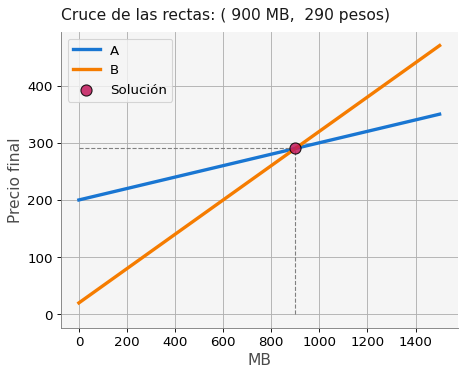
\includegraphics{03_derivadas_numericas_files/figure-pdf/cell-15-output-1.png}

\#\# Diferencias finitas centradas.

\$ \displaystyle \frac{\partial u(x)}{\partial x}
\approx \lim\limits\_\{h\to 0\} \frac{u(x+h) - u(x-h)}{2h} \$

La siguiente función de Python implementa la aproximación de
\textbf{diferencias finitas centradás}.

\begin{Shaded}
\begin{Highlighting}[]
\KeywordTok{def}\NormalTok{ centeredFD(u,x,h):}
    \CommentTok{""" }
\CommentTok{    Esquema de diferencias finitas centradas.}
\CommentTok{    }
\CommentTok{    Parameters}
\CommentTok{    {-}{-}{-}{-}{-}{-}{-}{-}{-}{-}}
\CommentTok{    u : función. }
\CommentTok{    Función a evaluar.}
\CommentTok{    }
\CommentTok{    x : array}
\CommentTok{    Lugar(es) donde se evalúa la función}
\CommentTok{    }
\CommentTok{    h : array}
\CommentTok{    Tamaño(s) de la diferencia entre u(x+h) y u(x).}
\CommentTok{    }
\CommentTok{    Returns}
\CommentTok{    {-}{-}{-}{-}{-}{-}{-}}
\CommentTok{    Cálculo de la derivada numérica centrada.}
\CommentTok{    """}
    \ControlFlowTok{return}\NormalTok{ (u(x}\OperatorTok{+}\NormalTok{h)}\OperatorTok{{-}}\NormalTok{u(x}\OperatorTok{{-}}\NormalTok{h))}\OperatorTok{/}\NormalTok{(}\DecValTok{2}\OperatorTok{*}\NormalTok{h)}
\end{Highlighting}
\end{Shaded}

\section{Ejercicio 2.}\label{ejercicio-2.}

Tomando como base el ejercicio 1, calcula el error entre la derivada
exacta y la aproximación con diferencias finitas centradas usando la
fórmula:

\[
Error = || \cos(x) - D_0 \sin(x)||
\]

donde \(D_0\) representa la aplicación de la fórmula de diferencias
centradas.

\begin{Shaded}
\begin{Highlighting}[]
\CommentTok{\# Metemos la información de h y del error en un Dataframe y mostramos el resultado:}
\CommentTok{\#\#\# }\RegionMarkerTok{BEGIN}\CommentTok{ SOLUTION}
\CommentTok{\# Calculamos el error entre la derivada exacta y la derivada numérica:}
\NormalTok{ec }\OperatorTok{=}\NormalTok{ np.fabs( np.cos(x) }\OperatorTok{{-}}\NormalTok{ centeredFD(np.sin,x,h) )}

\NormalTok{file\_answer.write(}\StringTok{\textquotesingle{}2\textquotesingle{}}\NormalTok{, ec, }\StringTok{\textquotesingle{}La implementación del error no es correcta, checa también los valores que estás comparando.\textquotesingle{}}\NormalTok{)}
\CommentTok{\#\#\# }\RegionMarkerTok{END}\CommentTok{ SOLUTION}

\BuiltInTok{print}\NormalTok{(ec)}
\end{Highlighting}
\end{Shaded}

\begin{verbatim}
El directorio :/home/jovyan/macti_notes/notebooks/.ans/DerivadasNumericas/ ya existe
Respuestas y retroalimentación almacenadas.
[8.56535925e-02 2.22328579e-02 5.61058720e-03 1.40593842e-03
 3.51690617e-04 8.79355346e-05]
\end{verbatim}

\begin{Shaded}
\begin{Highlighting}[]
\NormalTok{quizz.eval\_numeric(}\StringTok{\textquotesingle{}2\textquotesingle{}}\NormalTok{, ec)}
\end{Highlighting}
\end{Shaded}

\begin{verbatim}
----------------------------------------
2 | Tu resultado es correcto.
----------------------------------------
\end{verbatim}

\section{Ejercicio 3.}\label{ejercicio-3.}

Tomando como base los ejemplos de diferencias finitas hacia adelante y
hacia atrás, agrega una columna con los resultados del error de la
aproximación de diferencias centradas en el DataFrame \texttt{Error}.

\begin{Shaded}
\begin{Highlighting}[]
\CommentTok{\# Agregamos la columna del error de diferencias finitas centradas}
\CommentTok{\# Error[\textquotesingle{}...\textquotesingle{}] = ...}

\CommentTok{\#\#\# }\RegionMarkerTok{BEGIN}\CommentTok{ SOLUTION}
\NormalTok{Error[}\StringTok{\textquotesingle{}$D\_0$\textquotesingle{}}\NormalTok{] }\OperatorTok{=}\NormalTok{ ec}
\NormalTok{Error}
\CommentTok{\#\#\# }\RegionMarkerTok{END}\CommentTok{ SOLUTION}
\NormalTok{Error}
\end{Highlighting}
\end{Shaded}

\begin{longtable}[]{@{}lllll@{}}
\toprule\noalign{}
& \$h\$ & \$D\_+\$ & \$D\_-\$ & \$D\_0\$ \\
\midrule\noalign{}
\endhead
\bottomrule\noalign{}
\endlastfoot
0 & 1.00000 & 0.472476 & 0.301169 & 0.085654 \\
1 & 0.50000 & 0.228254 & 0.183789 & 0.022233 \\
2 & 0.25000 & 0.110248 & 0.099027 & 0.005611 \\
3 & 0.12500 & 0.053929 & 0.051118 & 0.001406 \\
4 & 0.06250 & 0.026639 & 0.025936 & 0.000352 \\
5 & 0.03125 & 0.013235 & 0.013059 & 0.000088 \\
\end{longtable}

Observe que en este caso los errores son varios órdenes de magnitud más
pequeños. Para hacer una gráfica más representativa usaremos escala
\texttt{loglog}:

\begin{Shaded}
\begin{Highlighting}[]
\CommentTok{\# Hacemos el gráfico del error vs h}
\NormalTok{plt.plot(h, ef, }\StringTok{\textquotesingle{}\^{}{-}\textquotesingle{}}\NormalTok{, label}\OperatorTok{=}\StringTok{\textquotesingle{}$D\_+$\textquotesingle{}}\NormalTok{)}
\NormalTok{plt.plot(h, eb, }\StringTok{\textquotesingle{}v{-}\textquotesingle{}}\NormalTok{, label}\OperatorTok{=}\StringTok{\textquotesingle{}$D\_{-}$\textquotesingle{}}\NormalTok{)}
\NormalTok{plt.plot(h, ec, }\StringTok{\textquotesingle{}s{-}\textquotesingle{}}\NormalTok{, label}\OperatorTok{=}\StringTok{\textquotesingle{}$D\_0$\textquotesingle{}}\NormalTok{)}
\NormalTok{plt.xlabel(}\StringTok{\textquotesingle{}$h$\textquotesingle{}}\NormalTok{)}
\NormalTok{plt.ylabel(}\StringTok{\textquotesingle{}Error\textquotesingle{}}\NormalTok{)}
\NormalTok{plt.title(}\StringTok{\textquotesingle{}Aproximación de la derivada\textquotesingle{}}\NormalTok{)}
\NormalTok{plt.legend()}
\NormalTok{plt.grid()}
\NormalTok{plt.loglog()  }\CommentTok{\# Definimos la escala log{-}log}
\NormalTok{plt.show()}
\end{Highlighting}
\end{Shaded}

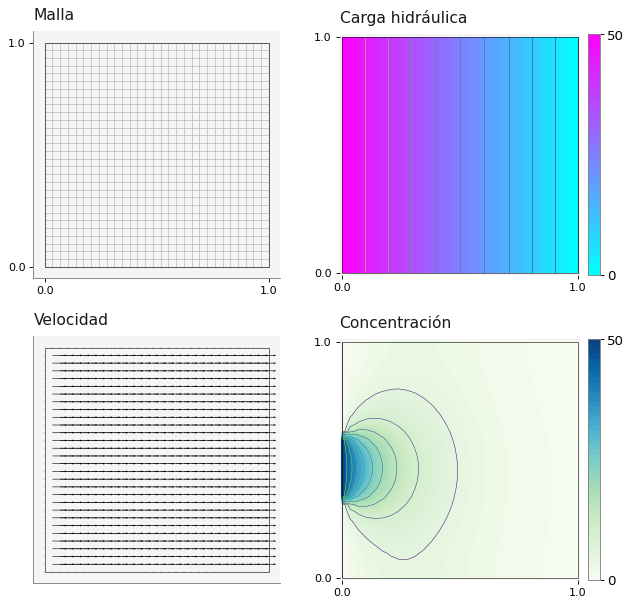
\includegraphics{03_derivadas_numericas_files/figure-pdf/cell-20-output-1.png}

Como se puede apreciar, la gráfica anterior muestra que la aproximación
con diferencias finitas centradas es mejor, pues es de orden cuadrático.

\section{Ejercicio 4. Aproximación con cuatro
puntos}\label{ejercicio-4.-aproximaciuxf3n-con-cuatro-puntos}

Implementar a siguiente fórmula de aproximación para el cálculo de la
primera derivada y usarla para calcular la derivada del \(\sin(x)\) en
\(x=1.0\) y compararla con las anteriores calculando el error y
graficando.

\[
D_3 u = \dfrac{1}{6 h} 
\left[ 2u_{i+1} + 3u_{i} - 6u_{i-1} + u_{i-2} \right]
\]

\textbf{Hint}: Recuerde que \(u_i = u(x)\), \(u_{i+1} = u(x+h)\),
\(u_{i-1} = u(x-h)\) y \(u_{i-2} = u(x-2h)\).

\begin{Shaded}
\begin{Highlighting}[]
\CommentTok{\# Implementación de D3}
\KeywordTok{def}\NormalTok{ D3(u,x,h):}
    \CommentTok{\#\#\# }\RegionMarkerTok{BEGIN}\CommentTok{ SOLUTION}
    \ControlFlowTok{return}\NormalTok{ (}\DecValTok{2}\OperatorTok{*}\NormalTok{u(x}\OperatorTok{+}\NormalTok{h)}\OperatorTok{+}\DecValTok{3}\OperatorTok{*}\NormalTok{u(x)}\OperatorTok{{-}}\DecValTok{6}\OperatorTok{*}\NormalTok{u(x}\OperatorTok{{-}}\NormalTok{h)}\OperatorTok{+}\NormalTok{u(x}\OperatorTok{{-}}\DecValTok{2}\OperatorTok{*}\NormalTok{h)) }\OperatorTok{/}\NormalTok{ (}\DecValTok{6}\OperatorTok{*}\NormalTok{h)}
    \CommentTok{\#\#\# }\RegionMarkerTok{END}\CommentTok{ SOLUTION}
\end{Highlighting}
\end{Shaded}

\begin{Shaded}
\begin{Highlighting}[]
\CommentTok{\#\#\# }\RegionMarkerTok{BEGIN}\CommentTok{ SOLUTION}
\CommentTok{\# Calculamos el error entre la derivada exacta y la derivada numérica:}
\NormalTok{e3 }\OperatorTok{=}\NormalTok{ np.fabs( np.cos(x) }\OperatorTok{{-}}\NormalTok{ D3(np.sin,x,h) )}

\NormalTok{file\_answer.write(}\StringTok{\textquotesingle{}3\textquotesingle{}}\NormalTok{, e3, }\StringTok{\textquotesingle{}La implementación del error no es correcta, checa también los valores que estás comparando.\textquotesingle{}}\NormalTok{)}
\CommentTok{\#\#\# }\RegionMarkerTok{END}\CommentTok{ SOLUTION}

\BuiltInTok{print}\NormalTok{(e3)}
\end{Highlighting}
\end{Shaded}

\begin{verbatim}
El directorio :/home/jovyan/macti_notes/notebooks/.ans/DerivadasNumericas/ ya existe
Respuestas y retroalimentación almacenadas.
[4.32871647e-02 7.31425947e-03 1.01447520e-03 1.32213104e-04
 1.68339444e-05 2.12244935e-06]
\end{verbatim}

\begin{Shaded}
\begin{Highlighting}[]
\NormalTok{quizz.eval\_numeric(}\StringTok{\textquotesingle{}3\textquotesingle{}}\NormalTok{, e3)}
\end{Highlighting}
\end{Shaded}

\begin{verbatim}
----------------------------------------
3 | Tu resultado es correcto.
----------------------------------------
\end{verbatim}

\section{Ejercicio 5.}\label{ejercicio-5.}

Tomando como base los ejemplos de diferencias finitas anteriores, agrega
una columna con los resultados del error de la aproximación de
diferencias con cuatro puntos en el DataFrame \texttt{Error}.

\begin{Shaded}
\begin{Highlighting}[]
\CommentTok{\# Agregamos la columna del error de diferencias finitas centradas}
\CommentTok{\#\#\# }\RegionMarkerTok{BEGIN}\CommentTok{ SOLUTION}
\NormalTok{Error[}\StringTok{\textquotesingle{}$D\_3$\textquotesingle{}}\NormalTok{] }\OperatorTok{=}\NormalTok{ e3}

\CommentTok{\#\#\# }\RegionMarkerTok{END}\CommentTok{ SOLUTION}
\NormalTok{Error}
\end{Highlighting}
\end{Shaded}

\begin{longtable}[]{@{}llllll@{}}
\toprule\noalign{}
& \$h\$ & \$D\_+\$ & \$D\_-\$ & \$D\_0\$ & \$D\_3\$ \\
\midrule\noalign{}
\endhead
\bottomrule\noalign{}
\endlastfoot
0 & 1.00000 & 0.472476 & 0.301169 & 0.085654 & 0.043287 \\
1 & 0.50000 & 0.228254 & 0.183789 & 0.022233 & 0.007314 \\
2 & 0.25000 & 0.110248 & 0.099027 & 0.005611 & 0.001014 \\
3 & 0.12500 & 0.053929 & 0.051118 & 0.001406 & 0.000132 \\
4 & 0.06250 & 0.026639 & 0.025936 & 0.000352 & 0.000017 \\
5 & 0.03125 & 0.013235 & 0.013059 & 0.000088 & 0.000002 \\
\end{longtable}

\begin{Shaded}
\begin{Highlighting}[]
\CommentTok{\# Hacemos el gráfico del error vs h}
\NormalTok{plt.plot(h, ef, }\StringTok{\textquotesingle{}\^{}{-}\textquotesingle{}}\NormalTok{, label}\OperatorTok{=}\StringTok{\textquotesingle{}$D\_+$\textquotesingle{}}\NormalTok{)}
\NormalTok{plt.plot(h, eb, }\StringTok{\textquotesingle{}v{-}\textquotesingle{}}\NormalTok{, label}\OperatorTok{=}\StringTok{\textquotesingle{}$D\_{-}$\textquotesingle{}}\NormalTok{)}
\NormalTok{plt.plot(h, ec, }\StringTok{\textquotesingle{}s{-}\textquotesingle{}}\NormalTok{, label}\OperatorTok{=}\StringTok{\textquotesingle{}$D\_0$\textquotesingle{}}\NormalTok{)}
\NormalTok{plt.plot(h, e3, }\StringTok{\textquotesingle{}o{-}\textquotesingle{}}\NormalTok{, label}\OperatorTok{=}\StringTok{\textquotesingle{}$D\_3$\textquotesingle{}}\NormalTok{)}

\NormalTok{plt.xlabel(}\StringTok{\textquotesingle{}$h$\textquotesingle{}}\NormalTok{)}
\NormalTok{plt.ylabel(}\StringTok{\textquotesingle{}Error\textquotesingle{}}\NormalTok{)}
\NormalTok{plt.title(}\StringTok{\textquotesingle{}Aproximación de la derivada\textquotesingle{}}\NormalTok{)}
\NormalTok{plt.legend()}
\NormalTok{plt.loglog()  }\CommentTok{\# Definimos la escala log{-}log}
\NormalTok{plt.grid()}
\NormalTok{plt.show()}
\end{Highlighting}
\end{Shaded}

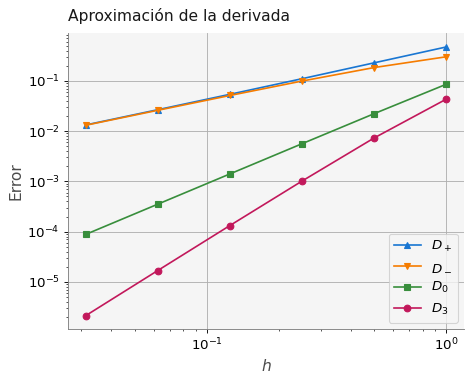
\includegraphics{03_derivadas_numericas_files/figure-pdf/cell-25-output-1.png}

\section{Ejercicio 6. Aproximación con tres puntos
(left).}\label{ejercicio-6.-aproximaciuxf3n-con-tres-puntos-left.}

Implementar a siguiente fórmula de aproximación para el cálculo de la
primera derivada y usarla para calcular la derivada del \(\sin(x)\) en
\(x=1.0\) y compararla con las anteriores.

\[
D_{2l}f^\prime = \frac{3 f_i - 4 f_{i-1} + f_{i-2}}{2h}
\]

\begin{Shaded}
\begin{Highlighting}[]
\CommentTok{\# Implementación}
\KeywordTok{def}\NormalTok{ D2l(u,x,h):}
    \CommentTok{\#\#\# }\RegionMarkerTok{BEGIN}\CommentTok{ SOLUTION}
    \ControlFlowTok{return}\NormalTok{ (}\DecValTok{3}\OperatorTok{*}\NormalTok{u(x) }\OperatorTok{{-}} \DecValTok{4}\OperatorTok{*}\NormalTok{u(x}\OperatorTok{{-}}\NormalTok{h) }\OperatorTok{+}\NormalTok{ u(x}\OperatorTok{{-}}\DecValTok{2}\OperatorTok{*}\NormalTok{h)) }\OperatorTok{/}\NormalTok{ (}\DecValTok{2}\OperatorTok{*}\NormalTok{h)}
    \CommentTok{\#\#\# }\RegionMarkerTok{END}\CommentTok{ SOLUTION}
\end{Highlighting}
\end{Shaded}

\begin{Shaded}
\begin{Highlighting}[]
\CommentTok{\#\#\# }\RegionMarkerTok{BEGIN}\CommentTok{ SOLUTION}
\CommentTok{\# Calculamos el error entre la derivada exacta y la derivada numérica:}
\NormalTok{e2l }\OperatorTok{=}\NormalTok{ np.fabs( np.cos(x) }\OperatorTok{{-}}\NormalTok{ D2l(np.sin,x,h) )}

\NormalTok{file\_answer.write(}\StringTok{\textquotesingle{}4\textquotesingle{}}\NormalTok{, e2l, }\StringTok{\textquotesingle{}La implementación del error no es correcta, checa también los valores que estás comparando.\textquotesingle{}}\NormalTok{)}
\CommentTok{\#\#\# }\RegionMarkerTok{END}\CommentTok{ SOLUTION}

\BuiltInTok{print}\NormalTok{(e2l)}
\end{Highlighting}
\end{Shaded}

\begin{verbatim}
El directorio :/home/jovyan/macti_notes/notebooks/.ans/DerivadasNumericas/ ya existe
Respuestas y retroalimentación almacenadas.
[3.01168679e-01 6.64084941e-02 1.42646000e-02 3.20851614e-03
 7.53883067e-04 1.82238417e-04]
\end{verbatim}

\begin{Shaded}
\begin{Highlighting}[]
\NormalTok{quizz.eval\_numeric(}\StringTok{\textquotesingle{}4\textquotesingle{}}\NormalTok{, e2l)}
\end{Highlighting}
\end{Shaded}

\begin{verbatim}
----------------------------------------
4 | Tu resultado es correcto.
----------------------------------------
\end{verbatim}

\section{Ejercicio 7.}\label{ejercicio-7.}

Tomando como base los ejemplos de diferencias finitas anteriores, agrega
una columna con los resultados del error de la aproximación de
diferencias con tres puntos-left en el DataFrame \texttt{Error}.

\begin{Shaded}
\begin{Highlighting}[]
\CommentTok{\# Colocamos la información de h y del error en un Dataframe y mostramos el resultado:}
\CommentTok{\#\#\# }\RegionMarkerTok{BEGIN}\CommentTok{ SOLUTION}
\NormalTok{Error[}\StringTok{\textquotesingle{}$D\_}\SpecialCharTok{\{2l\}}\StringTok{$\textquotesingle{}}\NormalTok{]}\OperatorTok{=}\NormalTok{e2l}

\CommentTok{\#\#\# }\RegionMarkerTok{END}\CommentTok{ SOLUTION}
\NormalTok{Error}
\end{Highlighting}
\end{Shaded}

\begin{longtable}[]{@{}lllllll@{}}
\toprule\noalign{}
& \$h\$ & \$D\_+\$ & \$D\_-\$ & \$D\_0\$ & \$D\_3\$ & \$D\_\{2l\}\$ \\
\midrule\noalign{}
\endhead
\bottomrule\noalign{}
\endlastfoot
0 & 1.00000 & 0.472476 & 0.301169 & 0.085654 & 0.043287 & 0.301169 \\
1 & 0.50000 & 0.228254 & 0.183789 & 0.022233 & 0.007314 & 0.066408 \\
2 & 0.25000 & 0.110248 & 0.099027 & 0.005611 & 0.001014 & 0.014265 \\
3 & 0.12500 & 0.053929 & 0.051118 & 0.001406 & 0.000132 & 0.003209 \\
4 & 0.06250 & 0.026639 & 0.025936 & 0.000352 & 0.000017 & 0.000754 \\
5 & 0.03125 & 0.013235 & 0.013059 & 0.000088 & 0.000002 & 0.000182 \\
\end{longtable}

\begin{Shaded}
\begin{Highlighting}[]
\CommentTok{\# Hacemos el gráfico del error vs h}
\NormalTok{plt.plot(h, ef, }\StringTok{\textquotesingle{}\^{}{-}\textquotesingle{}}\NormalTok{, label}\OperatorTok{=}\StringTok{\textquotesingle{}$D\_+$\textquotesingle{}}\NormalTok{)}
\NormalTok{plt.plot(h, eb, }\StringTok{\textquotesingle{}v{-}\textquotesingle{}}\NormalTok{, label}\OperatorTok{=}\StringTok{\textquotesingle{}$D\_{-}$\textquotesingle{}}\NormalTok{)}
\NormalTok{plt.plot(h, ec, }\StringTok{\textquotesingle{}s{-}\textquotesingle{}}\NormalTok{, label}\OperatorTok{=}\StringTok{\textquotesingle{}$D\_0$\textquotesingle{}}\NormalTok{)}
\NormalTok{plt.plot(h, e3, }\StringTok{\textquotesingle{}o{-}\textquotesingle{}}\NormalTok{, label}\OperatorTok{=}\StringTok{\textquotesingle{}$D\_3$\textquotesingle{}}\NormalTok{)}
\NormalTok{plt.plot(h, e2l, }\StringTok{\textquotesingle{}P{-}{-}\textquotesingle{}}\NormalTok{, label}\OperatorTok{=}\StringTok{\textquotesingle{}$D\_}\SpecialCharTok{\{2l\}}\StringTok{$\textquotesingle{}}\NormalTok{)}

\NormalTok{plt.xlabel(}\StringTok{\textquotesingle{}$h$\textquotesingle{}}\NormalTok{)}
\NormalTok{plt.ylabel(}\StringTok{\textquotesingle{}Error\textquotesingle{}}\NormalTok{)}
\NormalTok{plt.title(}\StringTok{\textquotesingle{}Aproximación de la derivada\textquotesingle{}}\NormalTok{)}
\NormalTok{plt.legend()}
\NormalTok{plt.loglog()  }\CommentTok{\# Definimos la escala log{-}log}
\NormalTok{plt.grid()}
\NormalTok{plt.show()}
\end{Highlighting}
\end{Shaded}

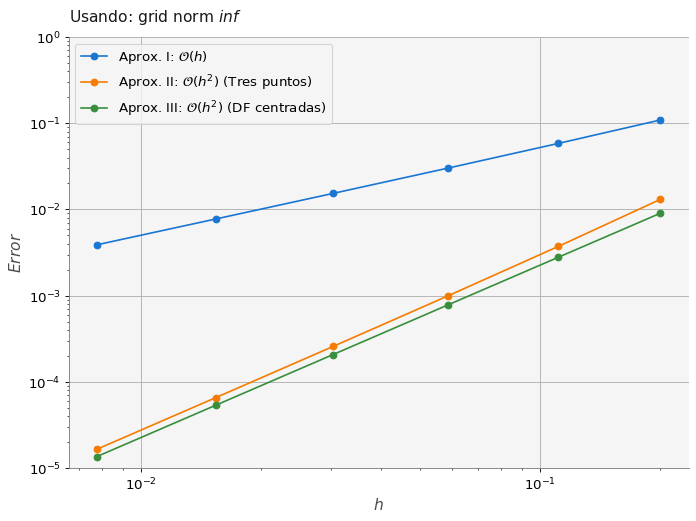
\includegraphics{03_derivadas_numericas_files/figure-pdf/cell-30-output-1.png}

\section{Ejercicio 6. Aproximación con tres puntos
(right).}\label{ejercicio-6.-aproximaciuxf3n-con-tres-puntos-right.}

Obtener los coeficientes \(A\), \(B\) y \(C\) para una aproximación del
siguiente tipo:

\[
D_{2r} f^\prime = A f_i + B f_{i+1} + C f_{i+2}
\]

y luego implementar la fórmula y graficarla junto con los resultados
anteriores.

\begin{Shaded}
\begin{Highlighting}[]
\CommentTok{\# Implementación}
\KeywordTok{def}\NormalTok{ D2r(u,x,h):}
    \CommentTok{\#\#\# }\RegionMarkerTok{BEGIN}\CommentTok{ SOLUTION}
    \ControlFlowTok{return}\NormalTok{ (}\OperatorTok{{-}}\DecValTok{3}\OperatorTok{*}\NormalTok{u(x) }\OperatorTok{+} \DecValTok{4}\OperatorTok{*}\NormalTok{u(x}\OperatorTok{+}\NormalTok{h) }\OperatorTok{{-}}\NormalTok{ u(x}\OperatorTok{+}\DecValTok{2}\OperatorTok{*}\NormalTok{h)) }\OperatorTok{/}\NormalTok{ (}\DecValTok{2}\OperatorTok{*}\NormalTok{h)}
    \CommentTok{\#\#\# }\RegionMarkerTok{END}\CommentTok{ SOLUTION}
\end{Highlighting}
\end{Shaded}

\begin{Shaded}
\begin{Highlighting}[]
\CommentTok{\#\#\# }\RegionMarkerTok{BEGIN}\CommentTok{ SOLUTION}
\CommentTok{\# Calculamos el error entre la derivada exacta y la derivada numérica:}
\NormalTok{e2r }\OperatorTok{=}\NormalTok{ np.fabs( np.cos(x) }\OperatorTok{{-}}\NormalTok{ D2r(np.sin,x,h) )}

\NormalTok{file\_answer.write(}\StringTok{\textquotesingle{}5\textquotesingle{}}\NormalTok{, e2r, }\StringTok{\textquotesingle{}La implementación del error no es correcta, checa también los valores que estás comparando.\textquotesingle{}}\NormalTok{)}
\NormalTok{file\_answer.to\_file(}\StringTok{\textquotesingle{}q3\textquotesingle{}}\NormalTok{)}
\CommentTok{\#\#\# }\RegionMarkerTok{END}\CommentTok{ SOLUTION}

\BuiltInTok{print}\NormalTok{(e2r)}
\end{Highlighting}
\end{Shaded}

\begin{verbatim}
El directorio :/home/jovyan/macti_notes/notebooks/.ans/DerivadasNumericas/ ya existe
Respuestas y retroalimentación almacenadas.
[0.05447393 0.01596726 0.00775877 0.0023889  0.00065123 0.0001694 ]
\end{verbatim}

\begin{Shaded}
\begin{Highlighting}[]
\NormalTok{quizz.eval\_numeric(}\StringTok{\textquotesingle{}5\textquotesingle{}}\NormalTok{, e2r)}
\end{Highlighting}
\end{Shaded}

\begin{verbatim}
----------------------------------------
5 | Tu resultado es correcto.
----------------------------------------
\end{verbatim}

\section{Ejercicio 7.}\label{ejercicio-7.-1}

Tomando como base los ejemplos de diferencias finitas anteriores, agrega
una columna con los resultados del error de la aproximación de
diferencias con \textbf{tres puntos-right} en el DataFrame
\texttt{Error}.

\begin{Shaded}
\begin{Highlighting}[]
\CommentTok{\# Colocamos la información de h y del error en un Dataframe y mostramos el resultado:}
\CommentTok{\#\#\# }\RegionMarkerTok{BEGIN}\CommentTok{ SOLUTION}
\NormalTok{Error[}\StringTok{\textquotesingle{}$D\_}\SpecialCharTok{\{2r\}}\StringTok{$\textquotesingle{}}\NormalTok{] }\OperatorTok{=}\NormalTok{ e2r}

\CommentTok{\#\#\# }\RegionMarkerTok{END}\CommentTok{ SOLUTION}
\NormalTok{Error}
\end{Highlighting}
\end{Shaded}

\begin{longtable}[]{@{}llllllll@{}}
\toprule\noalign{}
& \$h\$ & \$D\_+\$ & \$D\_-\$ & \$D\_0\$ & \$D\_3\$ & \$D\_\{2l\}\$ &
\$D\_\{2r\}\$ \\
\midrule\noalign{}
\endhead
\bottomrule\noalign{}
\endlastfoot
0 & 1.00000 & 0.472476 & 0.301169 & 0.085654 & 0.043287 & 0.301169 &
0.054474 \\
1 & 0.50000 & 0.228254 & 0.183789 & 0.022233 & 0.007314 & 0.066408 &
0.015967 \\
2 & 0.25000 & 0.110248 & 0.099027 & 0.005611 & 0.001014 & 0.014265 &
0.007759 \\
3 & 0.12500 & 0.053929 & 0.051118 & 0.001406 & 0.000132 & 0.003209 &
0.002389 \\
4 & 0.06250 & 0.026639 & 0.025936 & 0.000352 & 0.000017 & 0.000754 &
0.000651 \\
5 & 0.03125 & 0.013235 & 0.013059 & 0.000088 & 0.000002 & 0.000182 &
0.000169 \\
\end{longtable}

\begin{Shaded}
\begin{Highlighting}[]
\CommentTok{\# Hacemos el gráfico del error vs h}
\NormalTok{plt.plot(h, ef, }\StringTok{\textquotesingle{}\^{}{-}\textquotesingle{}}\NormalTok{, label}\OperatorTok{=}\StringTok{\textquotesingle{}$D\_+$\textquotesingle{}}\NormalTok{)}
\NormalTok{plt.plot(h, eb, }\StringTok{\textquotesingle{}v{-}\textquotesingle{}}\NormalTok{, label}\OperatorTok{=}\StringTok{\textquotesingle{}$D\_{-}$\textquotesingle{}}\NormalTok{)}
\NormalTok{plt.plot(h, ec, }\StringTok{\textquotesingle{}s{-}\textquotesingle{}}\NormalTok{, label}\OperatorTok{=}\StringTok{\textquotesingle{}$D\_0$\textquotesingle{}}\NormalTok{)}
\NormalTok{plt.plot(h, e3, }\StringTok{\textquotesingle{}o{-}\textquotesingle{}}\NormalTok{, label}\OperatorTok{=}\StringTok{\textquotesingle{}$D\_3$\textquotesingle{}}\NormalTok{)}
\NormalTok{plt.plot(h, e2l, }\StringTok{\textquotesingle{}P{-}{-}\textquotesingle{}}\NormalTok{, label}\OperatorTok{=}\StringTok{\textquotesingle{}$D\_}\SpecialCharTok{\{2l\}}\StringTok{$\textquotesingle{}}\NormalTok{)}
\NormalTok{plt.plot(h, e2r, }\StringTok{\textquotesingle{}p{-}.\textquotesingle{}}\NormalTok{, label}\OperatorTok{=}\StringTok{\textquotesingle{}$D\_}\SpecialCharTok{\{2r\}}\StringTok{$\textquotesingle{}}\NormalTok{)}

\NormalTok{plt.xlabel(}\StringTok{\textquotesingle{}$h$\textquotesingle{}}\NormalTok{)}
\NormalTok{plt.ylabel(}\StringTok{\textquotesingle{}Error\textquotesingle{}}\NormalTok{)}
\NormalTok{plt.title(}\StringTok{\textquotesingle{}Aproximación de la derivada\textquotesingle{}}\NormalTok{)}
\NormalTok{plt.legend()}
\NormalTok{plt.loglog()  }\CommentTok{\# Definimos la escala log{-}log}
\NormalTok{plt.grid()}
\NormalTok{plt.show()}
\end{Highlighting}
\end{Shaded}

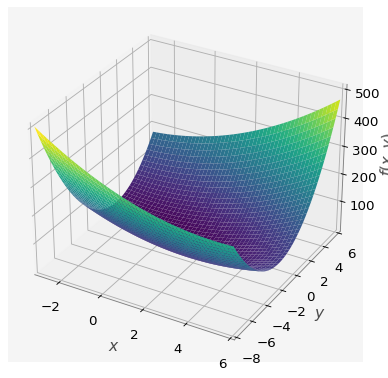
\includegraphics{03_derivadas_numericas_files/figure-pdf/cell-35-output-1.png}

\bookmarksetup{startatroot}

\chapter{Derivadas numéricas:
aplicación}\label{derivadas-numuxe9ricas-aplicaciuxf3n}

\textbf{Objetivo general} - Entender la utilidad de una derivada y su
aproximación numérica en una aplicación simple.

\begin{Shaded}
\begin{Highlighting}[]
\ImportTok{import}\NormalTok{ numpy }\ImportTok{as}\NormalTok{ np}
\ImportTok{import}\NormalTok{ matplotlib.pyplot }\ImportTok{as}\NormalTok{ plt}
\ImportTok{import}\NormalTok{ macti.visual }\ImportTok{as}\NormalTok{ mvis}
\ImportTok{from}\NormalTok{ macti.evaluation }\ImportTok{import} \OperatorTok{*}
\end{Highlighting}
\end{Shaded}

\begin{Shaded}
\begin{Highlighting}[]
\NormalTok{quizz }\OperatorTok{=}\NormalTok{ Quizz(}\StringTok{"q4"}\NormalTok{, }\StringTok{"notebooks"}\NormalTok{, }\StringTok{"local"}\NormalTok{)}
\end{Highlighting}
\end{Shaded}

\#\# Masa y densidad

Un experimentado maestro albañil, necesita cortar una varilla de metal
en varias secciones para construir una escalera. Realiza las marcas de
la varilla y se ven como en la siguiente figura:

Como se observa, el tamaño de cada sección de la varilla es de \(0.5\)
m. Por razones de la estructura, se necesita conocer el peso de cada
sección de la varilla para evitar que la escalera se derrumbe. El
maestro albañil realizó los cortes y pesó cada sección, obteniendo los
siguientes resultados:

\begin{longtable}[]{@{}
  >{\raggedright\arraybackslash}p{(\columnwidth - 16\tabcolsep) * \real{0.1111}}
  >{\raggedright\arraybackslash}p{(\columnwidth - 16\tabcolsep) * \real{0.1111}}
  >{\raggedright\arraybackslash}p{(\columnwidth - 16\tabcolsep) * \real{0.1111}}
  >{\raggedright\arraybackslash}p{(\columnwidth - 16\tabcolsep) * \real{0.1111}}
  >{\raggedright\arraybackslash}p{(\columnwidth - 16\tabcolsep) * \real{0.1111}}
  >{\raggedright\arraybackslash}p{(\columnwidth - 16\tabcolsep) * \real{0.1111}}
  >{\raggedright\arraybackslash}p{(\columnwidth - 16\tabcolsep) * \real{0.1111}}
  >{\raggedright\arraybackslash}p{(\columnwidth - 16\tabcolsep) * \real{0.1111}}
  >{\raggedright\arraybackslash}p{(\columnwidth - 16\tabcolsep) * \real{0.1111}}@{}}
\toprule\noalign{}
\begin{minipage}[b]{\linewidth}\raggedright
Sección
\end{minipage} & \begin{minipage}[b]{\linewidth}\raggedright
1
\end{minipage} & \begin{minipage}[b]{\linewidth}\raggedright
2
\end{minipage} & \begin{minipage}[b]{\linewidth}\raggedright
3
\end{minipage} & \begin{minipage}[b]{\linewidth}\raggedright
4
\end{minipage} & \begin{minipage}[b]{\linewidth}\raggedright
5
\end{minipage} & \begin{minipage}[b]{\linewidth}\raggedright
6
\end{minipage} & \begin{minipage}[b]{\linewidth}\raggedright
7
\end{minipage} & \begin{minipage}[b]{\linewidth}\raggedright
8
\end{minipage} \\
\midrule\noalign{}
\endhead
\bottomrule\noalign{}
\endlastfoot
Masa {[}Kg{]} & 0.595 & 0.806 & 0.369 & 1.078 & 1.704 & 1.475 & 2.263 &
3.282 \\
\end{longtable}

\section{Ejercicio 1.}\label{ejercicio-1.-2}

Definir los arreglos de \texttt{numpy} para las secciones de la varilla
como sigue:

\begin{enumerate}
\def\labelenumi{\alph{enumi}.}
\item
  \texttt{longitud} : para almacenar las marcas hechas en la varillas,
  comenzando en \(0\) y terminando en \(4.0\).
\item
  \texttt{masas\_sec}: para almacenar el valor de la masa de cada
  sección.
\end{enumerate}

\begin{Shaded}
\begin{Highlighting}[]
\CommentTok{\# longitud = np...}
\CommentTok{\# masas\_sec = np...}

\CommentTok{\#\#\# }\RegionMarkerTok{BEGIN}\CommentTok{ SOLUTION}
\CommentTok{\# Marcas sobre la varilla de cada sección}
\NormalTok{longitud }\OperatorTok{=}\NormalTok{ np.linspace(}\DecValTok{0}\NormalTok{,}\FloatTok{4.0}\NormalTok{,}\DecValTok{9}\NormalTok{)}
\CommentTok{\#np.array([0.0, 0.5, 1.0, 1.5, 2.0, 2.5, 3.0, 3.5,  4.0]) }

\CommentTok{\# Peso de cada sección [kg]}
\NormalTok{masas\_sec }\OperatorTok{=}\NormalTok{ np.array([}\FloatTok{0.595}\NormalTok{, }\FloatTok{0.806}\NormalTok{, }\FloatTok{0.369}\NormalTok{, }\FloatTok{1.078}\NormalTok{, }\FloatTok{1.704}\NormalTok{, }\FloatTok{1.475}\NormalTok{, }\FloatTok{2.263}\NormalTok{,  }\FloatTok{3.282}\NormalTok{])}

\NormalTok{file\_answer }\OperatorTok{=}\NormalTok{ FileAnswer()}
\NormalTok{file\_answer.write(}\StringTok{"1a"}\NormalTok{, longitud, }\StringTok{\textquotesingle{}Checa el arreglo secciones\textquotesingle{}}\NormalTok{)}
\NormalTok{file\_answer.write(}\StringTok{"1b"}\NormalTok{, masas\_sec, }\StringTok{\textquotesingle{}Checa el arreglo masas\_sec\textquotesingle{}}\NormalTok{)}
\CommentTok{\#\#\# }\RegionMarkerTok{END}\CommentTok{ SOLUTION}

\BuiltInTok{print}\NormalTok{(}\StringTok{\textquotesingle{}Longitud = }\SpecialCharTok{\{\}}\StringTok{\textquotesingle{}}\NormalTok{.}\BuiltInTok{format}\NormalTok{(longitud))}
\BuiltInTok{print}\NormalTok{(}\StringTok{\textquotesingle{}Masas = }\SpecialCharTok{\{\}}\StringTok{\textquotesingle{}}\NormalTok{.}\BuiltInTok{format}\NormalTok{(longitud))}
\end{Highlighting}
\end{Shaded}

\begin{verbatim}
El directorio :/home/jovyan/macti_notes/notebooks/.ans/DerivadasNumericas/ ya existe
Respuestas y retroalimentación almacenadas.
Longitud = [0.  0.5 1.  1.5 2.  2.5 3.  3.5 4. ]
Masas = [0.  0.5 1.  1.5 2.  2.5 3.  3.5 4. ]
\end{verbatim}

\begin{Shaded}
\begin{Highlighting}[]
\NormalTok{quizz.eval\_numeric(}\StringTok{\textquotesingle{}1a\textquotesingle{}}\NormalTok{,longitud)}
\end{Highlighting}
\end{Shaded}

\begin{verbatim}
----------------------------------------
1a | Tu resultado es correcto.
----------------------------------------
\end{verbatim}

\begin{Shaded}
\begin{Highlighting}[]
\NormalTok{quizz.eval\_numeric(}\StringTok{\textquotesingle{}1b\textquotesingle{}}\NormalTok{, masas\_sec)}
\end{Highlighting}
\end{Shaded}

\begin{verbatim}
----------------------------------------
1b | Tu resultado es correcto.
----------------------------------------
\end{verbatim}

\begin{Shaded}
\begin{Highlighting}[]
\CommentTok{\# Gráfica de la masa para cada sección en forma de barras verticales.}
\NormalTok{plt.bar(longitud[}\DecValTok{1}\NormalTok{:], masas\_sec, }
\NormalTok{        width}\OperatorTok{=}\FloatTok{0.1}\NormalTok{, color}\OperatorTok{=}\StringTok{\textquotesingle{}C3\textquotesingle{}}\NormalTok{, }
\NormalTok{        label}\OperatorTok{=}\StringTok{\textquotesingle{}Masa de cada sección de la varilla\textquotesingle{}}\NormalTok{)}

\NormalTok{plt.xlabel(}\StringTok{\textquotesingle{}Longitud [m]\textquotesingle{}}\NormalTok{)}
\NormalTok{plt.ylabel(}\StringTok{\textquotesingle{}Masa [kg]\textquotesingle{}}\NormalTok{)}
\NormalTok{plt.grid()}
\NormalTok{plt.legend()}
\NormalTok{plt.show()}
\end{Highlighting}
\end{Shaded}

\includegraphics{04_derivadas_numericas_aplicacion_files/figure-pdf/cell-7-output-1.png}

\section{Ejercicio 2.}\label{ejercicio-2.-1}

Escribe un código que genere el arreglo de numpy \texttt{masa} con
ceros, del mismo tamaño que el arreglo \texttt{longitud}. En la primera
posición del arreglo \texttt{masa} deje el valor de cero; en la segunda
posición ponga el valor de la masa de la primera sección; en la tercera
posición el valor de la primera sección más el valor de la masa de la
segunda sección; y así sucesivamente hasta obtener el peso total de la
varilla en la última posición. Diseñe un algoritmo para realizar este
proceso y escríbalo en la siguiente celda.

\begin{Shaded}
\begin{Highlighting}[]
\CommentTok{\# masa = ... \# arreglo para almacenar la masa de las secciones}
\CommentTok{\# for ...}
\CommentTok{\#     ...}

\CommentTok{\#\#\# }\RegionMarkerTok{BEGIN}\CommentTok{ SOLUTION}
\NormalTok{masa }\OperatorTok{=}\NormalTok{ np.zeros(}\BuiltInTok{len}\NormalTok{(longitud))}
\ControlFlowTok{for}\NormalTok{ i, ms }\KeywordTok{in} \BuiltInTok{enumerate}\NormalTok{(masas\_sec):}
\NormalTok{    masa[i}\OperatorTok{+}\DecValTok{1}\NormalTok{] }\OperatorTok{=}\NormalTok{ masa[i] }\OperatorTok{+}\NormalTok{ ms}
    
\NormalTok{file\_answer.write(}\StringTok{"2"}\NormalTok{, masa, }\StringTok{\textquotesingle{}Checa la construcción del arreglo masa\textquotesingle{}}\NormalTok{)}
\CommentTok{\#\#\# }\RegionMarkerTok{END}\CommentTok{ SOLUTION}

\BuiltInTok{print}\NormalTok{(}\StringTok{\textquotesingle{}Masa = }\SpecialCharTok{\{\}}\StringTok{\textquotesingle{}}\NormalTok{.}\BuiltInTok{format}\NormalTok{(masa))}
\end{Highlighting}
\end{Shaded}

\begin{verbatim}
El directorio :/home/jovyan/macti_notes/notebooks/.ans/DerivadasNumericas/ ya existe
Respuestas y retroalimentación almacenadas.
Masa = [ 0.     0.595  1.401  1.77   2.848  4.552  6.027  8.29  11.572]
\end{verbatim}

\begin{Shaded}
\begin{Highlighting}[]
\NormalTok{quizz.eval\_numeric(}\StringTok{\textquotesingle{}2\textquotesingle{}}\NormalTok{, masa)}
\end{Highlighting}
\end{Shaded}

\begin{verbatim}
----------------------------------------
2 | Tu resultado es correcto.
----------------------------------------
\end{verbatim}

\begin{Shaded}
\begin{Highlighting}[]
\CommentTok{\# Gráfica de la masa como función de la posición}
\NormalTok{plt.plot(longitud, masa, }
         \StringTok{\textquotesingle{}o{-}\textquotesingle{}}\NormalTok{, label}\OperatorTok{=}\StringTok{\textquotesingle{}Masa acumulada de la varilla\textquotesingle{}}\NormalTok{)}

\CommentTok{\# Gráfica de la masa para cada sección en forma de barras verticales.}
\NormalTok{plt.bar(longitud[}\DecValTok{1}\NormalTok{:], masas\_sec, }
\NormalTok{        width}\OperatorTok{=}\FloatTok{0.1}\NormalTok{, color}\OperatorTok{=}\StringTok{\textquotesingle{}C3\textquotesingle{}}\NormalTok{, }
\NormalTok{        label}\OperatorTok{=}\StringTok{\textquotesingle{}Masa de cada sección de varilla\textquotesingle{}}\NormalTok{)}

\NormalTok{plt.xlabel(}\StringTok{\textquotesingle{}Longitud [m]\textquotesingle{}}\NormalTok{)}
\NormalTok{plt.ylabel(}\StringTok{\textquotesingle{}Masa [kg]\textquotesingle{}}\NormalTok{)}
\NormalTok{plt.legend()}
\NormalTok{plt.grid()}
\NormalTok{plt.show()}
\end{Highlighting}
\end{Shaded}

\includegraphics{04_derivadas_numericas_aplicacion_files/figure-pdf/cell-10-output-1.png}

Si todo se hizo correctamente, se verá que la masa no crece linealmente.
Se sospecha que la densidad de la varilla no cambia homogéneamente en
toda su longitud. ¿Cómo podemos determinar la densidad de la varilla en
cada uno de sus puntos?

\begin{longtable}[]{@{}
  >{\raggedright\arraybackslash}p{(\columnwidth - 0\tabcolsep) * \real{0.5694}}@{}}
\toprule\noalign{}
\begin{minipage}[b]{\linewidth}\raggedright
Suponemos que todo está en una dimensión, de tal manera que podemos
definir una densidad ``lineal'' de la siguiente manera:
\end{minipage} \\
\midrule\noalign{}
\endhead
\bottomrule\noalign{}
\endlastfoot
3 \textbar{} Tu resultado es correcto. \\
\end{longtable}

\begin{verbatim}
:::
:::


::: {.cell nbgrader='{"grade":false,"grade_id":"cell-fde016e0198c4d2e","locked":false,"schema_version":3,"solution":true,"task":false}' execution_count=18}
``` {.python .cell-code}
# Gráfica de la masa y de la densidad para cada sección
plt.plot(longitud, masa, 'o-', label='Masa')
plt.plot(longitud[1:], densidad,'s-', label='Densidad')

# Gráfica de la masa para cada sección en forma de barras verticales.
plt.bar(longitud[1:], masas_sec, 
        width=0.1, color='C3', 
        label='Masa de cada sección de varilla')

plt.xlabel('Longitud [m]')
plt.ylabel('Masa [kg]')
plt.legend()
plt.grid()
plt.show()
\end{verbatim}

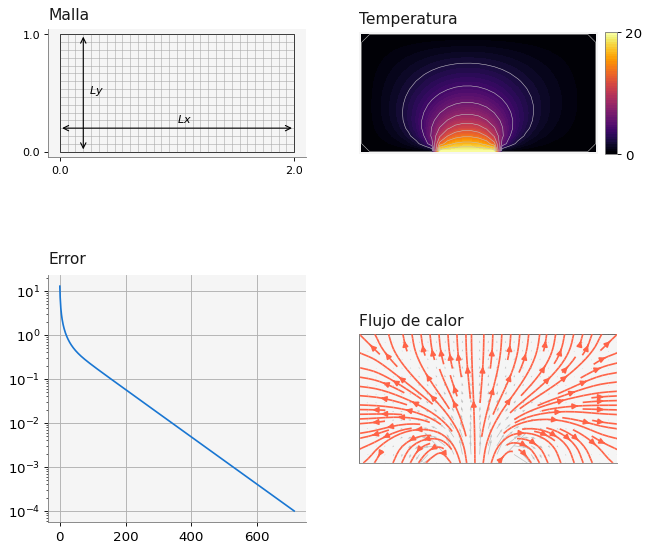
\includegraphics{04_derivadas_numericas_aplicacion_files/figure-pdf/cell-13-output-1.png}

:::

Después de una búsqueda sobre las especificaciones de la varilla, se
encuentra que la densidad está dada por siguiente fórmula:

\[
\rho = (1000 x^2 + 5000 \sin^2(2x)) A \tag{2}
\]

donde \(x\) es la posición en la varilla y \(A\) es el área transversal
de la misma. Al medir el diámetro de la varilla se encuentra el valor de
\(d = 0.02\) m , por lo tanto el radio es \(r = 0.01\) m.

\section{Ejercicio 4.}\label{ejercicio-4.}

Implemente la fórmula de la densidad \((2)\) en la función
\texttt{calc\_densidad(x,\ A)} y evalúa dicha fórmula con los datos del
radio antes definido y puntos que están en el intervalo \([0, 4.5]\)
separados por una distancia de \(0.1\). Almacena el resultado en la
variable ρ. Posteriormente compara gráficamente el resultado con la
aproximación realizada en el ejercicio anterior.

\begin{Shaded}
\begin{Highlighting}[]
\NormalTok{r }\OperatorTok{=} \FloatTok{0.01}
\NormalTok{A }\OperatorTok{=}\NormalTok{ np.pi }\OperatorTok{*}\NormalTok{ r }\OperatorTok{**} \DecValTok{2}

\CommentTok{\# def calc\_densidad(x, A):}
\CommentTok{\#     ...}
\CommentTok{\#}
\CommentTok{\# x = ...}
\CommentTok{\# ρ = ...}

\CommentTok{\#\#\# }\RegionMarkerTok{BEGIN}\CommentTok{ SOLUTION}
\NormalTok{calc\_densidad }\OperatorTok{=} \KeywordTok{lambda}\NormalTok{ x, A: (}\DecValTok{1000} \OperatorTok{*}\NormalTok{ x}\OperatorTok{**}\DecValTok{2} \OperatorTok{+} \DecValTok{5000} \OperatorTok{*}\NormalTok{ np.sin(}\DecValTok{2}\OperatorTok{*}\NormalTok{x)}\OperatorTok{**}\DecValTok{2}\NormalTok{) }\OperatorTok{*}\NormalTok{ A}

\CommentTok{\#def calc\_densidad(x, A):}
\CommentTok{\#    return (1000 * x**2 + 5000 * np.sin(2*x)**2) * A}

\CommentTok{\# Puntos donde se evaluá la fórmula de la densidad}
\NormalTok{x }\OperatorTok{=}\NormalTok{ np.arange(}\FloatTok{0.0}\NormalTok{, }\FloatTok{4.5}\NormalTok{, }\FloatTok{.1}\NormalTok{)}

\CommentTok{\# Cálculo de la densidad en cada posición del arreglo x}
\NormalTok{ρ }\OperatorTok{=}\NormalTok{ [calc\_densidad(l,A) }\ControlFlowTok{for}\NormalTok{ l }\KeywordTok{in}\NormalTok{ x]}
    
\NormalTok{file\_answer.write(}\StringTok{"4"}\NormalTok{, ρ, }\StringTok{\textquotesingle{}Verifica que la fórmula (2) esté bien implementada y cada uno de los datos de entrada.\textquotesingle{}}\NormalTok{)}
\CommentTok{\#\#\# }\RegionMarkerTok{END}\CommentTok{ SOLUTION}
\NormalTok{file\_answer.to\_file(}\StringTok{\textquotesingle{}q4\textquotesingle{}}\NormalTok{)}

\BuiltInTok{print}\NormalTok{(ρ)}
\end{Highlighting}
\end{Shaded}

\begin{verbatim}
El directorio :/home/jovyan/macti_notes/notebooks/.ans/DerivadasNumericas/ ya existe
Respuestas y retroalimentación almacenadas.
[0.0, 0.065140142984144, 0.25077236406386394, 0.5290773824209537, 0.8585968970424002, 1.1907789408649767, 1.4776431688135958, 1.6793558992965574, 1.7705189766656613, 1.7441795815382646, 1.6129279280991666, 1.406909546114531, 1.169065964621893, 0.9483551886937212, 0.7920223069253689, 0.7381405307711528, 0.8096002716097072, 1.0104952481017955, 1.3254761780264852, 1.7221740924437288, 2.156310684160917, 2.578688878846925, 2.9429599713234333, 3.212941066996997, 3.368327565325648, 3.4078988097868033, 3.349710802702375, 3.2282455594876254, 3.0889671566078496, 2.9811439535688815, 2.9500702022640968, 3.0299150805307193, 3.238328130281404, 3.5736527829144573, 4.0151878950714055, 4.526456003996436, 5.060962316838884, 5.569535216116573, 6.00808937693044, 6.344585870417729, 6.564090406147258, 6.671131128203245, 6.688983720799259, 6.65599668952679, 6.619536975529502]
\end{verbatim}

\begin{Shaded}
\begin{Highlighting}[]
\NormalTok{quizz.eval\_numeric(}\StringTok{\textquotesingle{}4\textquotesingle{}}\NormalTok{,ρ)}
\end{Highlighting}
\end{Shaded}

\begin{verbatim}
----------------------------------------
4 | Tu resultado es correcto.
----------------------------------------
\end{verbatim}

\begin{Shaded}
\begin{Highlighting}[]
\CommentTok{\# Gráfica de la masa como función de las secciones}
\NormalTok{plt.plot(longitud, masa, }\StringTok{\textquotesingle{}o{-}\textquotesingle{}}\NormalTok{, label}\OperatorTok{=}\StringTok{\textquotesingle{}Masa\textquotesingle{}}\NormalTok{)}

\CommentTok{\# Gráfica de la densidad como función de las secciones}
\NormalTok{plt.plot(longitud[}\DecValTok{1}\NormalTok{:], densidad,}\StringTok{\textquotesingle{}s{-}\textquotesingle{}}\NormalTok{, label}\OperatorTok{=}\StringTok{\textquotesingle{}Densidad\textquotesingle{}}\NormalTok{)}

\CommentTok{\# Gráfica de la densidad exacta}
\NormalTok{plt.plot(x, ρ, label }\OperatorTok{=} \StringTok{\textquotesingle{}$}\CharTok{\textbackslash{}\textbackslash{}}\StringTok{rho =(1000 x\^{}2 + 5000 \textbackslash{}sin(2x)\^{}2 ) * A $\textquotesingle{}}\NormalTok{)}

\CommentTok{\# Gráfica de la masa para cada sección en forma de barras verticales.}
\NormalTok{plt.bar(longitud[}\DecValTok{1}\NormalTok{:], masas\_sec, }
\NormalTok{        width}\OperatorTok{=}\FloatTok{0.1}\NormalTok{, color}\OperatorTok{=}\StringTok{\textquotesingle{}C3\textquotesingle{}}\NormalTok{, }
\NormalTok{        label}\OperatorTok{=}\StringTok{\textquotesingle{}Masa de cada sección de varilla\textquotesingle{}}\NormalTok{)}

\NormalTok{plt.xlabel(}\StringTok{\textquotesingle{}Longitud [m]\textquotesingle{}}\NormalTok{)}
\NormalTok{plt.ylabel(}\StringTok{\textquotesingle{}Masa [kg]\textquotesingle{}}\NormalTok{)}
\NormalTok{plt.legend()}
\NormalTok{plt.grid()}
\NormalTok{plt.show()}
\end{Highlighting}
\end{Shaded}

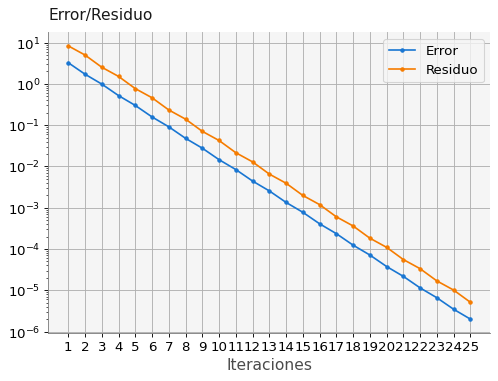
\includegraphics{04_derivadas_numericas_aplicacion_files/figure-pdf/cell-16-output-1.png}

Para evaluar la aproximación, se puede usar el error absoluto y el error
relativo los cuales se definen como sigue.

\[
\begin{eqnarray*}
Error_{absoluto} & = & ||v_e - v_a|| \\ \\
Error_{relativo} & = & \dfrac{||v_e - v_a||}{||v_e||}
\end{eqnarray*}
\]

donde \(v_e\) es el valor exacto y \(v_a\) es el valor aproximado.

\section{Ejercicio 5. Error absoluto y error
relativo.}\label{ejercicio-5.-error-absoluto-y-error-relativo.}

Implemente las fórmulas del error absoluto y relativo en las funciones
\emph{lambda} \texttt{error\_absoluto(ve,\ va)} y
\texttt{error\_relativo(ve,\ va)} respectivamente.

\begin{itemize}
\tightlist
\item
  5a. Calcular el valor de la densidad exacta con la fórmula (2) para
  cada sección. Almacene el resultado en la variable
  \texttt{densidad\_e}.
\item
  5b. Comparar la aproximación (1) con el resultado del inciso 5a usando
  el error absoluto. Almacene el error en la variable \texttt{error\_a}.
\item
  5c. Comparar la aproximación (1) con el resultado del inciso 5a usando
  el error relativo. Almacene el error en la variable \texttt{error\_r}.
\end{itemize}

\begin{Shaded}
\begin{Highlighting}[]
\CommentTok{\# error\_absoluto = lambda ...}
\CommentTok{\# error\_relativo = lambda ...}
\CommentTok{\# densidad\_e = ...}
\CommentTok{\# error\_a = ...}
\CommentTok{\# error\_r = ...}

\CommentTok{\#\#\# }\RegionMarkerTok{BEGIN}\CommentTok{ SOLUTION}
\NormalTok{error\_absoluto }\OperatorTok{=} \KeywordTok{lambda}\NormalTok{ ve, va: np.fabs(ve }\OperatorTok{{-}}\NormalTok{ va)}
\NormalTok{error\_relativo }\OperatorTok{=} \KeywordTok{lambda}\NormalTok{ ve, va: np.fabs(ve }\OperatorTok{{-}}\NormalTok{ va) }\OperatorTok{/}\NormalTok{ np.fabs(ve)}

\CommentTok{\# Calculamos la densidad en cada sección con la fórmula (2)}
\NormalTok{densidad\_e }\OperatorTok{=}\NormalTok{ calc\_densidad(longitud[}\DecValTok{1}\NormalTok{:], A)}

\CommentTok{\# Calculamos los errores con respecto de la aproximación}

\NormalTok{error\_a }\OperatorTok{=}\NormalTok{ [error\_absoluto(e, a) }\ControlFlowTok{for}\NormalTok{ e, a }\KeywordTok{in} \BuiltInTok{zip}\NormalTok{(densidad\_e, densidad)]}
\NormalTok{error\_r }\OperatorTok{=}\NormalTok{ [error\_relativo(e, a) }\ControlFlowTok{for}\NormalTok{ e, a }\KeywordTok{in} \BuiltInTok{zip}\NormalTok{(densidad\_e, densidad)]}

\CommentTok{\#error\_a = []}
\CommentTok{\#error\_r = []}
\CommentTok{\#for e,a in zip(densidad\_e, densidad):}
\CommentTok{\#    error\_a.append(error\_absoluto(e,a))}
\CommentTok{\#    error\_r.append(error\_relativo(e,a))}
    
\NormalTok{file\_answer.write(}\StringTok{"5a"}\NormalTok{, densidad\_e, }\StringTok{\textquotesingle{}\textquotesingle{}}\NormalTok{)}
\NormalTok{file\_answer.write(}\StringTok{"5b"}\NormalTok{, error\_a, }\StringTok{\textquotesingle{}\textquotesingle{}}\NormalTok{)}
\NormalTok{file\_answer.write(}\StringTok{"5c"}\NormalTok{, error\_r, }\StringTok{\textquotesingle{}\textquotesingle{}}\NormalTok{)}
\CommentTok{\#\#\# }\RegionMarkerTok{END}\CommentTok{ SOLUTION}

\BuiltInTok{print}\NormalTok{(}\StringTok{\textquotesingle{}Densidad exacta secciones = }\SpecialCharTok{\{\}}\CharTok{\textbackslash{}n}\StringTok{\textquotesingle{}}\NormalTok{.}\BuiltInTok{format}\NormalTok{(densidad\_e))}
\BuiltInTok{print}\NormalTok{(}\StringTok{\textquotesingle{}Error absoluto = }\SpecialCharTok{\{\}}\CharTok{\textbackslash{}n}\StringTok{\textquotesingle{}}\NormalTok{.}\BuiltInTok{format}\NormalTok{(error\_a))}
\BuiltInTok{print}\NormalTok{(}\StringTok{\textquotesingle{}Error relativo = }\SpecialCharTok{\{\}}\CharTok{\textbackslash{}n}\StringTok{\textquotesingle{}}\NormalTok{.}\BuiltInTok{format}\NormalTok{(error\_r))}
\end{Highlighting}
\end{Shaded}

\begin{verbatim}
Densidad exacta secciones = [1.19077894 1.61292793 0.73814053 2.15631068 3.40789881 2.9500702
 4.526456   6.56409041]

Error absoluto = [0.0007789408649767626, 0.0009279280991665306, 0.00014053077115283585, 0.00031068416091750706, 0.00010119021319621169, 7.020226409748531e-05, 0.00045600399643586087, 9.040614725819296e-05]

Error relativo = [0.0006541439710135815, 0.0005753066104200283, 0.0001903848458314842, 0.0001440813530256208, 2.969284560492631e-05, 2.3796811358457512e-05, 0.0001007419482335081, 1.3772837006255698e-05]
\end{verbatim}

\begin{Shaded}
\begin{Highlighting}[]
\NormalTok{quizz.eval\_numeric(}\StringTok{\textquotesingle{}5a\textquotesingle{}}\NormalTok{, densidad\_e)}
\end{Highlighting}
\end{Shaded}

\begin{verbatim}
----------------------------------------
5a | Tu resultado es correcto.
----------------------------------------
\end{verbatim}

\begin{Shaded}
\begin{Highlighting}[]
\NormalTok{quizz.eval\_numeric(}\StringTok{\textquotesingle{}5b\textquotesingle{}}\NormalTok{, error\_a)}
\end{Highlighting}
\end{Shaded}

\begin{verbatim}
----------------------------------------
5b | Tu resultado es correcto.
----------------------------------------
\end{verbatim}

\begin{Shaded}
\begin{Highlighting}[]
\NormalTok{quizz.eval\_numeric(}\StringTok{\textquotesingle{}5c\textquotesingle{}}\NormalTok{, error\_r)}
\end{Highlighting}
\end{Shaded}

\begin{verbatim}
----------------------------------------
5c | Tu resultado es correcto.
----------------------------------------
\end{verbatim}

\begin{Shaded}
\begin{Highlighting}[]
\CommentTok{\# Gráficas del error absoluto y del error relativo}
\NormalTok{plt.plot(longitud[}\DecValTok{1}\NormalTok{:], error\_a, }\StringTok{\textquotesingle{}o{-}\textquotesingle{}}\NormalTok{, label}\OperatorTok{=}\StringTok{\textquotesingle{}Error Absoluto\textquotesingle{}}\NormalTok{)}
\NormalTok{plt.plot(longitud[}\DecValTok{1}\NormalTok{:], error\_r, }\StringTok{\textquotesingle{}o{-}\textquotesingle{}}\NormalTok{, label}\OperatorTok{=}\StringTok{\textquotesingle{}Error Relativo\textquotesingle{}}\NormalTok{)}
\NormalTok{plt.legend()}
\NormalTok{plt.grid()}
\NormalTok{plt.show()}
\end{Highlighting}
\end{Shaded}

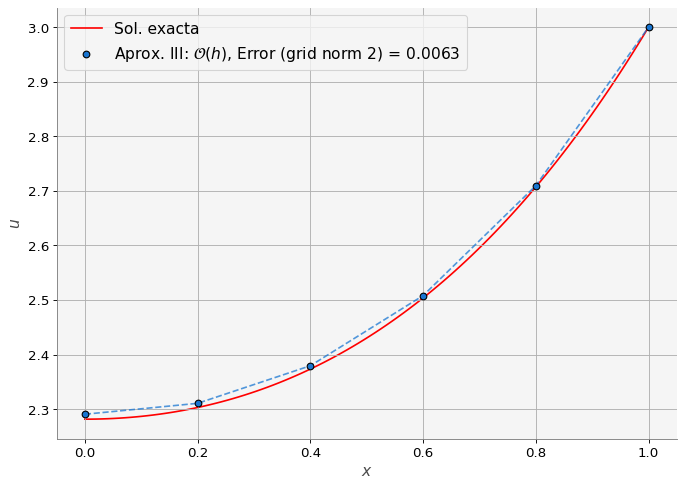
\includegraphics{04_derivadas_numericas_aplicacion_files/figure-pdf/cell-21-output-1.png}

Si tenemos la fórmula de la densidad, ecuación \((2)\), podemos
encontrar la fórmula para la masa haciendo la integral de la densidad.

\[
m(x) = \int \rho dx = \int (1000 x^2 + 5000 \sin^2(2x)) A \; dx = A \int f(x) \; dx = ¿? \tag{3}
\]

\section{Ejercicio 5. Fórmula exacta para la
masa.}\label{ejercicio-5.-fuxf3rmula-exacta-para-la-masa.}

\begin{itemize}
\tightlist
\item
  6a. Cálcula la integral definida en \((3)\) donde
  \(f(x) = 1000 x^2 + 5000 \sin^2(2x)\) . Escribe su respuesta en la
  variable \texttt{masa\_e} usando expresiones de Python y funciones de
  Sympy.
\item
  6b. Posteriormente calcula la masa para cada sección usando el
  resultado de la integración. Para ello escribe una función
  \emph{lambda} con la fórmula de la integral. Almacena el resultado en
  la variable \texttt{m}.
\end{itemize}

Compare el resultado gráficamente con los datos de la masa calculados al
inicio.

\textbf{NOTA}. Puede usar Sympy para calcular la integral.

\begin{Shaded}
\begin{Highlighting}[]
\CommentTok{\# importamos funciones de sympy para escribir la respuesta.}
\ImportTok{from}\NormalTok{ sympy }\ImportTok{import}\NormalTok{ Symbol, sin, cos}

\CommentTok{\# definimos el símbolo x}
\NormalTok{x }\OperatorTok{=}\NormalTok{ Symbol(}\StringTok{\textquotesingle{}x\textquotesingle{}}\NormalTok{) }

\CommentTok{\# definimos la función original para la densidad}
\NormalTok{f }\OperatorTok{=} \DecValTok{1000} \OperatorTok{*}\NormalTok{ x}\OperatorTok{**}\DecValTok{2} \OperatorTok{+} \DecValTok{5000} \OperatorTok{*}\NormalTok{ sin(}\DecValTok{2}\OperatorTok{*}\NormalTok{x)}\OperatorTok{**}\DecValTok{2}

\CommentTok{\# masa\_e = ...}

\CommentTok{\#\#\# }\RegionMarkerTok{BEGIN}\CommentTok{ SOLUTION}
\CommentTok{\#from sympy import integrate}
\CommentTok{\#masa\_e = integrate(f, x)}

\NormalTok{masa\_e }\OperatorTok{=} \DecValTok{1000}\OperatorTok{*}\NormalTok{x}\OperatorTok{**}\DecValTok{3}\OperatorTok{/}\DecValTok{3} \OperatorTok{+} \DecValTok{2500}\OperatorTok{*}\NormalTok{x }\OperatorTok{{-}} \DecValTok{1250}\OperatorTok{*}\NormalTok{sin(}\DecValTok{2}\OperatorTok{*}\NormalTok{x)}\OperatorTok{*}\NormalTok{cos(}\DecValTok{2}\OperatorTok{*}\NormalTok{x)}

\NormalTok{file\_answer.write(}\StringTok{"6a"}\NormalTok{, }\BuiltInTok{str}\NormalTok{(masa\_e), }\StringTok{"Revisa el cálculo de la integral."}\NormalTok{)}
\CommentTok{\#\#\# }\RegionMarkerTok{END}\CommentTok{ SOLUTION}

\BuiltInTok{print}\NormalTok{(}\StringTok{"Densidad exacta:"}\NormalTok{)}
\NormalTok{display(f)}
\BuiltInTok{print}\NormalTok{(}\StringTok{"Masa exacta:"}\NormalTok{)}
\NormalTok{display(masa\_e)}
\end{Highlighting}
\end{Shaded}

\begin{verbatim}
El directorio :/home/jovyan/macti_notes/notebooks/.ans/DerivadasNumericas/ ya existe
Respuestas y retroalimentación almacenadas.
Densidad exacta:
Masa exacta:
\end{verbatim}

$\displaystyle 1000 x^{2} + 5000 \sin^{2}{\left(2 x \right)}$

$\displaystyle \frac{1000 x^{3}}{3} + 2500 x - 1250 \sin{\left(2 x \right)} \cos{\left(2 x \right)}$

\begin{Shaded}
\begin{Highlighting}[]
\NormalTok{quizz.eval\_expression(}\StringTok{\textquotesingle{}6a\textquotesingle{}}\NormalTok{, masa\_e)}
\end{Highlighting}
\end{Shaded}

\begin{verbatim}
----------------------------------------
6a | Tu respuesta:
es correcta.
----------------------------------------
\end{verbatim}

$\displaystyle \frac{1000 x^{3}}{3} + 2500 x - 1250 \sin{\left(2 x \right)} \cos{\left(2 x \right)}$

\begin{Shaded}
\begin{Highlighting}[]
\CommentTok{\# Calcula la masa usando la fórmula exacta obtenida anteriormente.}
\CommentTok{\# calc\_masa = lambda x: ...}
\CommentTok{\# x = ...}
\CommentTok{\# m = ...}

\CommentTok{\#\#\# }\RegionMarkerTok{BEGIN}\CommentTok{ SOLUTION}
\NormalTok{calc\_masa }\OperatorTok{=} \KeywordTok{lambda}\NormalTok{ x: (}\DecValTok{1000} \OperatorTok{*}\NormalTok{ x}\OperatorTok{**}\DecValTok{3} \OperatorTok{/} \DecValTok{3} \OperatorTok{+} \DecValTok{2500}\OperatorTok{*}\NormalTok{x }\OperatorTok{{-}} \DecValTok{1250} \OperatorTok{*}\NormalTok{ np.sin(}\DecValTok{2}\OperatorTok{*}\NormalTok{x) }\OperatorTok{*}\NormalTok{ np.cos(}\DecValTok{2}\OperatorTok{*}\NormalTok{x) ) }\OperatorTok{*}\NormalTok{ A}
\NormalTok{x }\OperatorTok{=}\NormalTok{ np.arange(}\FloatTok{0.0}\NormalTok{, }\FloatTok{4.5}\NormalTok{, }\FloatTok{.1}\NormalTok{)}
\NormalTok{m }\OperatorTok{=}\NormalTok{ [calc\_masa(l) }\ControlFlowTok{for}\NormalTok{ l }\KeywordTok{in}\NormalTok{ x]}

\NormalTok{file\_answer.write(}\StringTok{"6b"}\NormalTok{, m, }\StringTok{"Checa la implementación de la fórmula exacta para la masa."}\NormalTok{)}
\NormalTok{file\_answer.to\_file(}\StringTok{\textquotesingle{}q4\textquotesingle{}}\NormalTok{)}
\CommentTok{\#\#\# }\RegionMarkerTok{END}\CommentTok{ SOLUTION}

\BuiltInTok{print}\NormalTok{(}\StringTok{\textquotesingle{}Masa exacta = }\SpecialCharTok{\{\}}\StringTok{\textquotesingle{}}\NormalTok{.}\BuiltInTok{format}\NormalTok{(m))}
\end{Highlighting}
\end{Shaded}

\begin{verbatim}
El directorio :/home/jovyan/macti_notes/notebooks/.ans/DerivadasNumericas/ ya existe
Respuestas y retroalimentación almacenadas.
Masa exacta = [0.0, 0.002182423384241263, 0.017064851646832385, 0.05544143582414131, 0.1245955116842955, 0.2272489188359526, 0.3612314797824474, 0.519922820911168, 0.6933967815987044, 0.8700877343973358, 1.0387157409844714, 1.1901666040809675, 1.319029996479012, 1.4245528304264585, 1.510857351304525, 1.5863895234025789, 1.6626847955472912, 1.7526461050549453, 1.8686059853195873, 2.0204787276384506, 2.2142943302921436, 2.4513456920843106, 2.7280836897293286, 3.036776704061495, 3.3668304703789333, 3.7065598775737922, 4.045132987924423, 4.374380359569433, 4.6901840194284095, 4.993226798285815, 5.288983724504746, 5.586956835113887, 5.8992742107720435, 6.238874416184963, 6.617562982912055, 7.044247773193793, 7.523631822050594, 8.055570029143981, 8.6351912646101, 9.25376661103931, 9.900186665284211, 10.56281466662354, 11.231422883091394, 11.898906543147781, 12.56250472056554]
\end{verbatim}

\begin{Shaded}
\begin{Highlighting}[]
\NormalTok{quizz.eval\_numeric(}\StringTok{\textquotesingle{}6b\textquotesingle{}}\NormalTok{, m)}
\end{Highlighting}
\end{Shaded}

\begin{verbatim}
----------------------------------------
6b | Tu resultado es correcto.
----------------------------------------
\end{verbatim}

\begin{Shaded}
\begin{Highlighting}[]
\CommentTok{\# Gráfica de la masa exacta y de la aproximada}
\NormalTok{plt.plot(longitud, masa, }\StringTok{\textquotesingle{}o{-}\textquotesingle{}}\NormalTok{, label}\OperatorTok{=}\StringTok{\textquotesingle{}Masa aproximada\textquotesingle{}}\NormalTok{)}
\NormalTok{plt.plot(x, m, }\StringTok{\textquotesingle{}{-}\textquotesingle{}}\NormalTok{, label }\OperatorTok{=} \StringTok{\textquotesingle{}Masa exacta\textquotesingle{}}\NormalTok{)}

\NormalTok{plt.xlabel(}\StringTok{\textquotesingle{}Longitud [m]\textquotesingle{}}\NormalTok{)}
\NormalTok{plt.ylabel(}\StringTok{\textquotesingle{}Masa [kg]\textquotesingle{}}\NormalTok{)}
\NormalTok{plt.legend()}
\NormalTok{plt.grid()}
\NormalTok{plt.show()}
\end{Highlighting}
\end{Shaded}

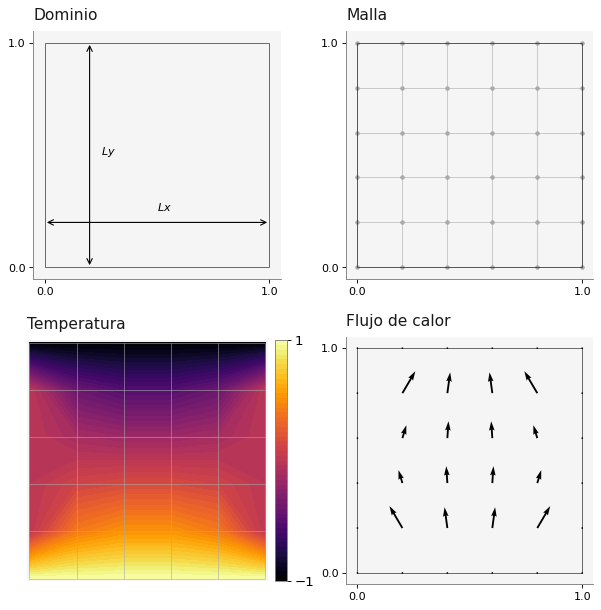
\includegraphics{04_derivadas_numericas_aplicacion_files/figure-pdf/cell-26-output-1.png}

\bookmarksetup{startatroot}

\chapter{Derivadas numéricas: ecuación de calor
1D.}\label{derivadas-numuxe9ricas-ecuaciuxf3n-de-calor-1d.}

\textbf{Objetivo}. - Aplicar diferencias finitas centradas en la
solución numérica de la transferencia de calor en 1D.

MACTI-Analisis\_Numerico\_01 by Luis M. de la Cruz is licensed under
Attribution-ShareAlike 4.0 International

\textbf{Trabajo realizado con el apoyo del Programa UNAM-DGAPA-PAPIME
PE101922}

\begin{Shaded}
\begin{Highlighting}[]
\ImportTok{import}\NormalTok{ numpy }\ImportTok{as}\NormalTok{ np}
\ImportTok{import}\NormalTok{ matplotlib.pyplot }\ImportTok{as}\NormalTok{ plt}
\ImportTok{import}\NormalTok{ pandas }\ImportTok{as}\NormalTok{ pd}
\ImportTok{import}\NormalTok{ ipywidgets }\ImportTok{as}\NormalTok{ widgets}
\ImportTok{import}\NormalTok{ macti.visual }\ImportTok{as}\NormalTok{ mvis}
\ImportTok{from}\NormalTok{ macti.evaluation }\ImportTok{import} \OperatorTok{*}
\end{Highlighting}
\end{Shaded}

\begin{Shaded}
\begin{Highlighting}[]
\NormalTok{quizz }\OperatorTok{=}\NormalTok{ Quizz(}\StringTok{\textquotesingle{}1\textquotesingle{}}\NormalTok{, }\StringTok{\textquotesingle{}notebooks\textquotesingle{}}\NormalTok{, }\StringTok{\textquotesingle{}local\textquotesingle{}}\NormalTok{)}
\end{Highlighting}
\end{Shaded}

El modelo matemático para la conducción de calor en 1D con condiciones
de frontera de tipo Dirichlet, con \(\kappa\) = constante se escribe
como sigue:

\[
\begin{eqnarray}
-\kappa \frac{d^2T}{dx^2} & = & S \; \text{ para } x \in [0,L] \\
T(x=0) & = & T_A \\
T(x=L) & = & T_B
\end{eqnarray}
\]

La solución analítica de este modelo matemático se escribe como sigue:

\[
T(x) =
\left(\frac{T_B - T_A}{L} + \frac{S}{2\kappa} \left(L - x\right) \right)x + T_A \tag{1}
\]

\section{Ejercicio 1.}\label{ejercicio-1.-3}

En la siguiente celda complete el código para implementar la fórmula
\((1)\). Posteriormente, define los siguientes valores para calcular la
solución exacta:

\begin{Shaded}
\begin{Highlighting}[]
\NormalTok{x}\OperatorTok{=}\NormalTok{np.linspace(}\DecValTok{0}\NormalTok{,}\DecValTok{1}\NormalTok{,}\DecValTok{10}\NormalTok{)}
\NormalTok{TA }\OperatorTok{=} \FloatTok{1.0}
\NormalTok{TB }\OperatorTok{=} \FloatTok{0.0}
\NormalTok{S }\OperatorTok{=} \FloatTok{1.0}
\NormalTok{L }\OperatorTok{=} \FloatTok{1.0}
\NormalTok{k }\OperatorTok{=} \FloatTok{1.0}
\end{Highlighting}
\end{Shaded}

\begin{Shaded}
\begin{Highlighting}[]
\CommentTok{\# Solucion exacta}
\KeywordTok{def}\NormalTok{ sol\_exacta(x, TA, TB, S, L, k):}
    \CommentTok{"""}
\CommentTok{    Calcula la temperatura usando la fórmula obtenida con Series de Taylor.}

\CommentTok{    Parameters}
\CommentTok{    {-}{-}{-}{-}{-}{-}{-}{-}{-}{-}}
\CommentTok{    x: np.array}
\CommentTok{    Coordenadas donde se calcula la temperatura.}

\CommentTok{    TA: float}
\CommentTok{    Es la condición de frontera a la izquierda.}
\CommentTok{    }
\CommentTok{    TB: float}
\CommentTok{    Es la condición de frontera a la derecha.}

\CommentTok{    S: float}
\CommentTok{    es la fuente.}
\CommentTok{    }
\CommentTok{    L: float}
\CommentTok{    L es la longitud del dominio.}
\CommentTok{    }
\CommentTok{    k: float}
\CommentTok{    es la conductividad del material.}
\CommentTok{    }
\CommentTok{    Return}
\CommentTok{    {-}{-}{-}{-}{-}{-}}
\CommentTok{    al final esta función dibuja la solución.}
\CommentTok{    """}
    \CommentTok{\#\#\# }\RegionMarkerTok{BEGIN}\CommentTok{ SOLUTION}
    \ControlFlowTok{return}\NormalTok{ ((TB }\OperatorTok{{-}}\NormalTok{ TA)}\OperatorTok{/}\NormalTok{L }\OperatorTok{+}\NormalTok{ S }\OperatorTok{/}\NormalTok{(}\DecValTok{2}\OperatorTok{*}\NormalTok{k) }\OperatorTok{*}\NormalTok{ (L }\OperatorTok{{-}}\NormalTok{ x) ) }\OperatorTok{*}\NormalTok{ x }\OperatorTok{+}\NormalTok{ TA}
    \CommentTok{\#\#\# }\RegionMarkerTok{END}\CommentTok{ SOLUTION}
\end{Highlighting}
\end{Shaded}

\begin{Shaded}
\begin{Highlighting}[]
\NormalTok{x}\OperatorTok{=}\NormalTok{np.linspace(}\DecValTok{0}\NormalTok{,}\DecValTok{1}\NormalTok{,}\DecValTok{10}\NormalTok{)}
\NormalTok{TA }\OperatorTok{=} \FloatTok{1.0}
\NormalTok{TB }\OperatorTok{=} \FloatTok{0.0}
\NormalTok{S }\OperatorTok{=} \FloatTok{1.0}
\NormalTok{L }\OperatorTok{=} \FloatTok{1.0}
\NormalTok{k }\OperatorTok{=} \FloatTok{1.0}

\CommentTok{\# Cálculo de la solución exacta.}
\CommentTok{\# Te = ...}
\CommentTok{\#\#\# }\RegionMarkerTok{BEGIN}\CommentTok{ SOLUTION}
\NormalTok{Te }\OperatorTok{=}\NormalTok{ sol\_exacta(x, TA, TB, S, L, k)}

\NormalTok{file\_answer }\OperatorTok{=}\NormalTok{ FileAnswer()}
\NormalTok{file\_answer.write(}\StringTok{"1"}\NormalTok{, Te, }\StringTok{\textquotesingle{}Checa el arreglo secciones\textquotesingle{}}\NormalTok{)}
\CommentTok{\#\#\# }\RegionMarkerTok{END}\CommentTok{ SOLUTION}

\BuiltInTok{print}\NormalTok{(}\StringTok{\textquotesingle{}T exacta = }\SpecialCharTok{\{\}}\StringTok{\textquotesingle{}}\NormalTok{,Te)}
\end{Highlighting}
\end{Shaded}

\begin{verbatim}
T exacta = {} [1.         0.9382716  0.86419753 0.77777778 0.67901235 0.56790123
 0.44444444 0.30864198 0.16049383 0.        ]
\end{verbatim}

\begin{Shaded}
\begin{Highlighting}[]
\NormalTok{quizz.eval\_numeric(}\StringTok{\textquotesingle{}1\textquotesingle{}}\NormalTok{, Te)}
\end{Highlighting}
\end{Shaded}

\begin{verbatim}
----------------------------------------
1 | Tu resultado es correcto.
----------------------------------------
\end{verbatim}

\section{Ejercicio 2. Error absoluto y error
relativo.}\label{ejercicio-2.-error-absoluto-y-error-relativo.}

El error absoluto y el error relativo se definen como sigue.

\[
\begin{eqnarray*}
Error_{absoluto} & = & ||v_e - v_a|| \\ \\
Error_{relativo} & = & \dfrac{||v_e - v_a||}{||v_e||}
\end{eqnarray*}
\]

donde \(v_e\) es el valor exacto y \(v_a\) es el valor aproximado.

Implementa las fórmulas del \(Error_{absoluto}\) y del
\(Error_{relativo}\) en la funciones \texttt{error\_absoluto()}~y
\texttt{error\_relativo()}, respectivamente.

\begin{Shaded}
\begin{Highlighting}[]
\KeywordTok{def}\NormalTok{ error\_absoluto(ve, va):}
    \CommentTok{"""}
\CommentTok{    Calcula el error absoluto entre el valor exacto (ve) y el valor aproximado (va).}
\CommentTok{    """}
    \CommentTok{\#\#\# }\RegionMarkerTok{BEGIN}\CommentTok{ SOLUTION}
    \ControlFlowTok{return}\NormalTok{ np.linalg.norm(ve }\OperatorTok{{-}}\NormalTok{ va)}
    \CommentTok{\#\#\# }\RegionMarkerTok{END}\CommentTok{ SOLUTION}
\end{Highlighting}
\end{Shaded}

\begin{Shaded}
\begin{Highlighting}[]
\KeywordTok{def}\NormalTok{ error\_relativo(ve, va):}
    \CommentTok{"""}
\CommentTok{    Calcula el error relativo entre el valor exacto (ve) y el valor aproximado (va).}
\CommentTok{    """}
    \CommentTok{\# }\RegionMarkerTok{BEGIN}\CommentTok{ SOLUTION}
    \ControlFlowTok{return}\NormalTok{ np.linalg.norm(ve }\OperatorTok{{-}}\NormalTok{ va) }\OperatorTok{/}\NormalTok{ np.linalg.norm(ve)}
    \CommentTok{\# }\RegionMarkerTok{END}\CommentTok{ SOLUTION}
\end{Highlighting}
\end{Shaded}

\section{Ejercicio 3. Solución numérica
(interactivo).}\label{ejercicio-3.-soluciuxf3n-numuxe9rica-interactivo.}

Si todo lo realizaste correctamente, ejecuta la siguiente celda para
generar un interativo. Mueve los valores de k, S y N y observa lo que
sucede.

\begin{Shaded}
\begin{Highlighting}[]
\KeywordTok{def}\NormalTok{ conduccion\_1d(k, S, L, TA, TB, N):}
    \CommentTok{"""}
\CommentTok{    Calcula la temperatura en 1D mediante diferencias finitas.}
\CommentTok{    }
\CommentTok{    Parameters}
\CommentTok{    {-}{-}{-}{-}{-}{-}{-}{-}{-}{-}    }
\CommentTok{    L: float}
\CommentTok{    L es la longitud del dominio.}
\CommentTok{    }
\CommentTok{    k: float}
\CommentTok{    es la conductividad del material.}
\CommentTok{    }
\CommentTok{    S: float}
\CommentTok{    es la fuente.}
\CommentTok{    }
\CommentTok{    TA: float}
\CommentTok{    Es la condición de frontera a la izquierda.}
\CommentTok{    }
\CommentTok{    TB: float}
\CommentTok{    Es la condición de frontera a la derecha.}

\CommentTok{    N: int}
\CommentTok{    Es el número de nodos internos (grados de libertad).}
\CommentTok{    }
\CommentTok{    Return}
\CommentTok{    {-}{-}{-}{-}{-}{-}}
\CommentTok{    al final esta función dibuja la solución.}
\CommentTok{    """}

    \CommentTok{\# Cálculo de algunos parámetros numéricos}
\NormalTok{    h }\OperatorTok{=}\NormalTok{ L }\OperatorTok{/}\NormalTok{ (N}\OperatorTok{+}\DecValTok{1}\NormalTok{)}
\NormalTok{    r }\OperatorTok{=}\NormalTok{ k }\OperatorTok{/}\NormalTok{ h}\OperatorTok{**}\DecValTok{2}
    
    \CommentTok{\# Definición de arreglos }
\NormalTok{    T }\OperatorTok{=}\NormalTok{ np.zeros(N}\OperatorTok{+}\DecValTok{2}\NormalTok{)}
\NormalTok{    b }\OperatorTok{=}\NormalTok{ np.zeros(N)}
\NormalTok{    A }\OperatorTok{=}\NormalTok{ np.zeros((N,N))}

    \CommentTok{\# Se inicializa todo el arreglo b con S/r}
\NormalTok{    b[:] }\OperatorTok{=}\NormalTok{ S }\OperatorTok{/}\NormalTok{ r}

    \CommentTok{\# Condiciones de frontera en el arreglo de la Temperatura.}
\NormalTok{    T[}\DecValTok{0}\NormalTok{] }\OperatorTok{=}\NormalTok{ TA}
\NormalTok{    T[}\OperatorTok{{-}}\DecValTok{1}\NormalTok{] }\OperatorTok{=}\NormalTok{ TB}
    
    \CommentTok{\# Se ajusta el vector del lado derecho (RHS) con las condiciones de frontera.}
\NormalTok{    b[}\DecValTok{0}\NormalTok{] }\OperatorTok{+=}\NormalTok{ TA}
\NormalTok{    b[}\OperatorTok{{-}}\DecValTok{1}\NormalTok{] }\OperatorTok{+=}\NormalTok{ TB}

    \CommentTok{\# Se calculan las entradas de la matriz del sistema de ecuaciones lineales.}
\NormalTok{    A[}\DecValTok{0}\NormalTok{,}\DecValTok{0}\NormalTok{] }\OperatorTok{=} \DecValTok{2}
\NormalTok{    A[}\DecValTok{0}\NormalTok{,}\DecValTok{1}\NormalTok{] }\OperatorTok{=} \OperatorTok{{-}}\DecValTok{1}
    \ControlFlowTok{for}\NormalTok{ i }\KeywordTok{in} \BuiltInTok{range}\NormalTok{(}\DecValTok{1}\NormalTok{,N}\OperatorTok{{-}}\DecValTok{1}\NormalTok{):}
\NormalTok{        A[i,i] }\OperatorTok{=} \DecValTok{2}
\NormalTok{        A[i,i}\OperatorTok{+}\DecValTok{1}\NormalTok{] }\OperatorTok{=} \OperatorTok{{-}}\DecValTok{1}
\NormalTok{        A[i,i}\OperatorTok{{-}}\DecValTok{1}\NormalTok{] }\OperatorTok{=} \OperatorTok{{-}}\DecValTok{1}
\NormalTok{    A[}\OperatorTok{{-}}\DecValTok{1}\NormalTok{,}\OperatorTok{{-}}\DecValTok{2}\NormalTok{] }\OperatorTok{=} \OperatorTok{{-}}\DecValTok{1}
\NormalTok{    A[}\OperatorTok{{-}}\DecValTok{1}\NormalTok{,}\OperatorTok{{-}}\DecValTok{1}\NormalTok{] }\OperatorTok{=} \DecValTok{2}

    \CommentTok{\# Se resuelve el sistema lineal.}
\NormalTok{    T[}\DecValTok{1}\NormalTok{:N}\OperatorTok{+}\DecValTok{1}\NormalTok{] }\OperatorTok{=}\NormalTok{ np.linalg.solve(A,b)}

    \CommentTok{\# Coordenadas para la solución exacta.}
\NormalTok{    xe }\OperatorTok{=}\NormalTok{ np.linspace(}\DecValTok{0}\NormalTok{,L,}\DecValTok{100}\NormalTok{)}
    
    \CommentTok{\# Coordenadas para la solución numérica.}
\NormalTok{    xa }\OperatorTok{=}\NormalTok{ np.linspace(}\DecValTok{0}\NormalTok{,L,N}\OperatorTok{+}\DecValTok{2}\NormalTok{)}
    
    \CommentTok{\# Se calcula la solución exacta en las coordenadas xe.}
\NormalTok{    Te }\OperatorTok{=}\NormalTok{ sol\_exacta(xe, TA, TB, S, L, k)}
    
    \CommentTok{\# Se calcula el error absoluto.}
\NormalTok{    ea }\OperatorTok{=}\NormalTok{ error\_absoluto(T, sol\_exacta(xa,TA,TB,S,L,k))}
    
    \CommentTok{\# Se calcula el error relativo}
\NormalTok{    er }\OperatorTok{=}\NormalTok{ error\_relativo(T, sol\_exacta(xa,TA,TB,S,L,k))}

    \CommentTok{\# Se imprime el error absoluto y el relativo.}
    \BuiltInTok{print}\NormalTok{(}\StringTok{\textquotesingle{}Error absoluto = }\SpecialCharTok{\{:6.5e\}}\StringTok{, Error relativo = }\SpecialCharTok{\{:6.5e\}}\StringTok{\textquotesingle{}}\NormalTok{.}\BuiltInTok{format}\NormalTok{(ea, er))}

    \CommentTok{\# Se realiza la gráfica de la solución.}
\NormalTok{    plt.plot(xa, T, }\StringTok{\textquotesingle{}o{-}\textquotesingle{}}\NormalTok{, lw }\OperatorTok{=} \FloatTok{0.5}\NormalTok{, c}\OperatorTok{=}\StringTok{\textquotesingle{}k\textquotesingle{}}\NormalTok{, label }\OperatorTok{=} \StringTok{\textquotesingle{}Numérica\textquotesingle{}}\NormalTok{, zorder}\OperatorTok{=}\DecValTok{5}\NormalTok{)}
\NormalTok{    plt.plot(xe, Te, lw}\OperatorTok{=}\DecValTok{5}\NormalTok{, c}\OperatorTok{=}\StringTok{\textquotesingle{}limegreen\textquotesingle{}}\NormalTok{, label }\OperatorTok{=} \StringTok{\textquotesingle{}Exacta\textquotesingle{}}\NormalTok{)}
\NormalTok{    plt.xlabel(}\StringTok{\textquotesingle{}$x$\textquotesingle{}}\NormalTok{)}
\NormalTok{    plt.ylabel(}\StringTok{\textquotesingle{}$T$\textquotesingle{}}\NormalTok{)}
\NormalTok{    plt.legend()}
\NormalTok{    plt.grid()}
\NormalTok{    plt.show()}
    
\CommentTok{\# Construcción del interactivo.}
\NormalTok{widgets.interactive(conduccion\_1d,}
\NormalTok{                    k }\OperatorTok{=}\NormalTok{ widgets.FloatSlider(}\BuiltInTok{max}\OperatorTok{=}\FloatTok{1.0}\NormalTok{, }\BuiltInTok{min}\OperatorTok{=}\FloatTok{0.02}\NormalTok{, value}\OperatorTok{=}\FloatTok{0.02}\NormalTok{, step}\OperatorTok{=}\FloatTok{0.1}\NormalTok{), }
\NormalTok{                    S }\OperatorTok{=}\NormalTok{ widgets.FloatSlider(}\BuiltInTok{max}\OperatorTok{=}\FloatTok{10.0}\NormalTok{, }\BuiltInTok{min}\OperatorTok{=}\FloatTok{0.0}\NormalTok{, value}\OperatorTok{=}\DecValTok{0}\NormalTok{, step}\OperatorTok{=}\FloatTok{1.0}\NormalTok{), }
\NormalTok{                    L }\OperatorTok{=}\NormalTok{ widgets.fixed(}\FloatTok{5.0}\NormalTok{), }
\NormalTok{                    TA }\OperatorTok{=}\NormalTok{ widgets.fixed(}\DecValTok{200}\NormalTok{), }
\NormalTok{                    TB }\OperatorTok{=}\NormalTok{ widgets.fixed(}\DecValTok{1000}\NormalTok{), }
\NormalTok{                    N }\OperatorTok{=}\NormalTok{ widgets.IntSlider(}\BuiltInTok{max}\OperatorTok{=}\DecValTok{10}\NormalTok{, }\BuiltInTok{min}\OperatorTok{=}\DecValTok{4}\NormalTok{, value}\OperatorTok{=}\DecValTok{4}\NormalTok{))}
\end{Highlighting}
\end{Shaded}

\begin{verbatim}
interactive(children=(FloatSlider(value=0.02, description='k', max=1.0, min=0.02), FloatSlider(value=0.0, desc…
\end{verbatim}



\end{document}
